
\section{Pyörävaellus 9.–12.5.}

\begin{Figure}
	\noindent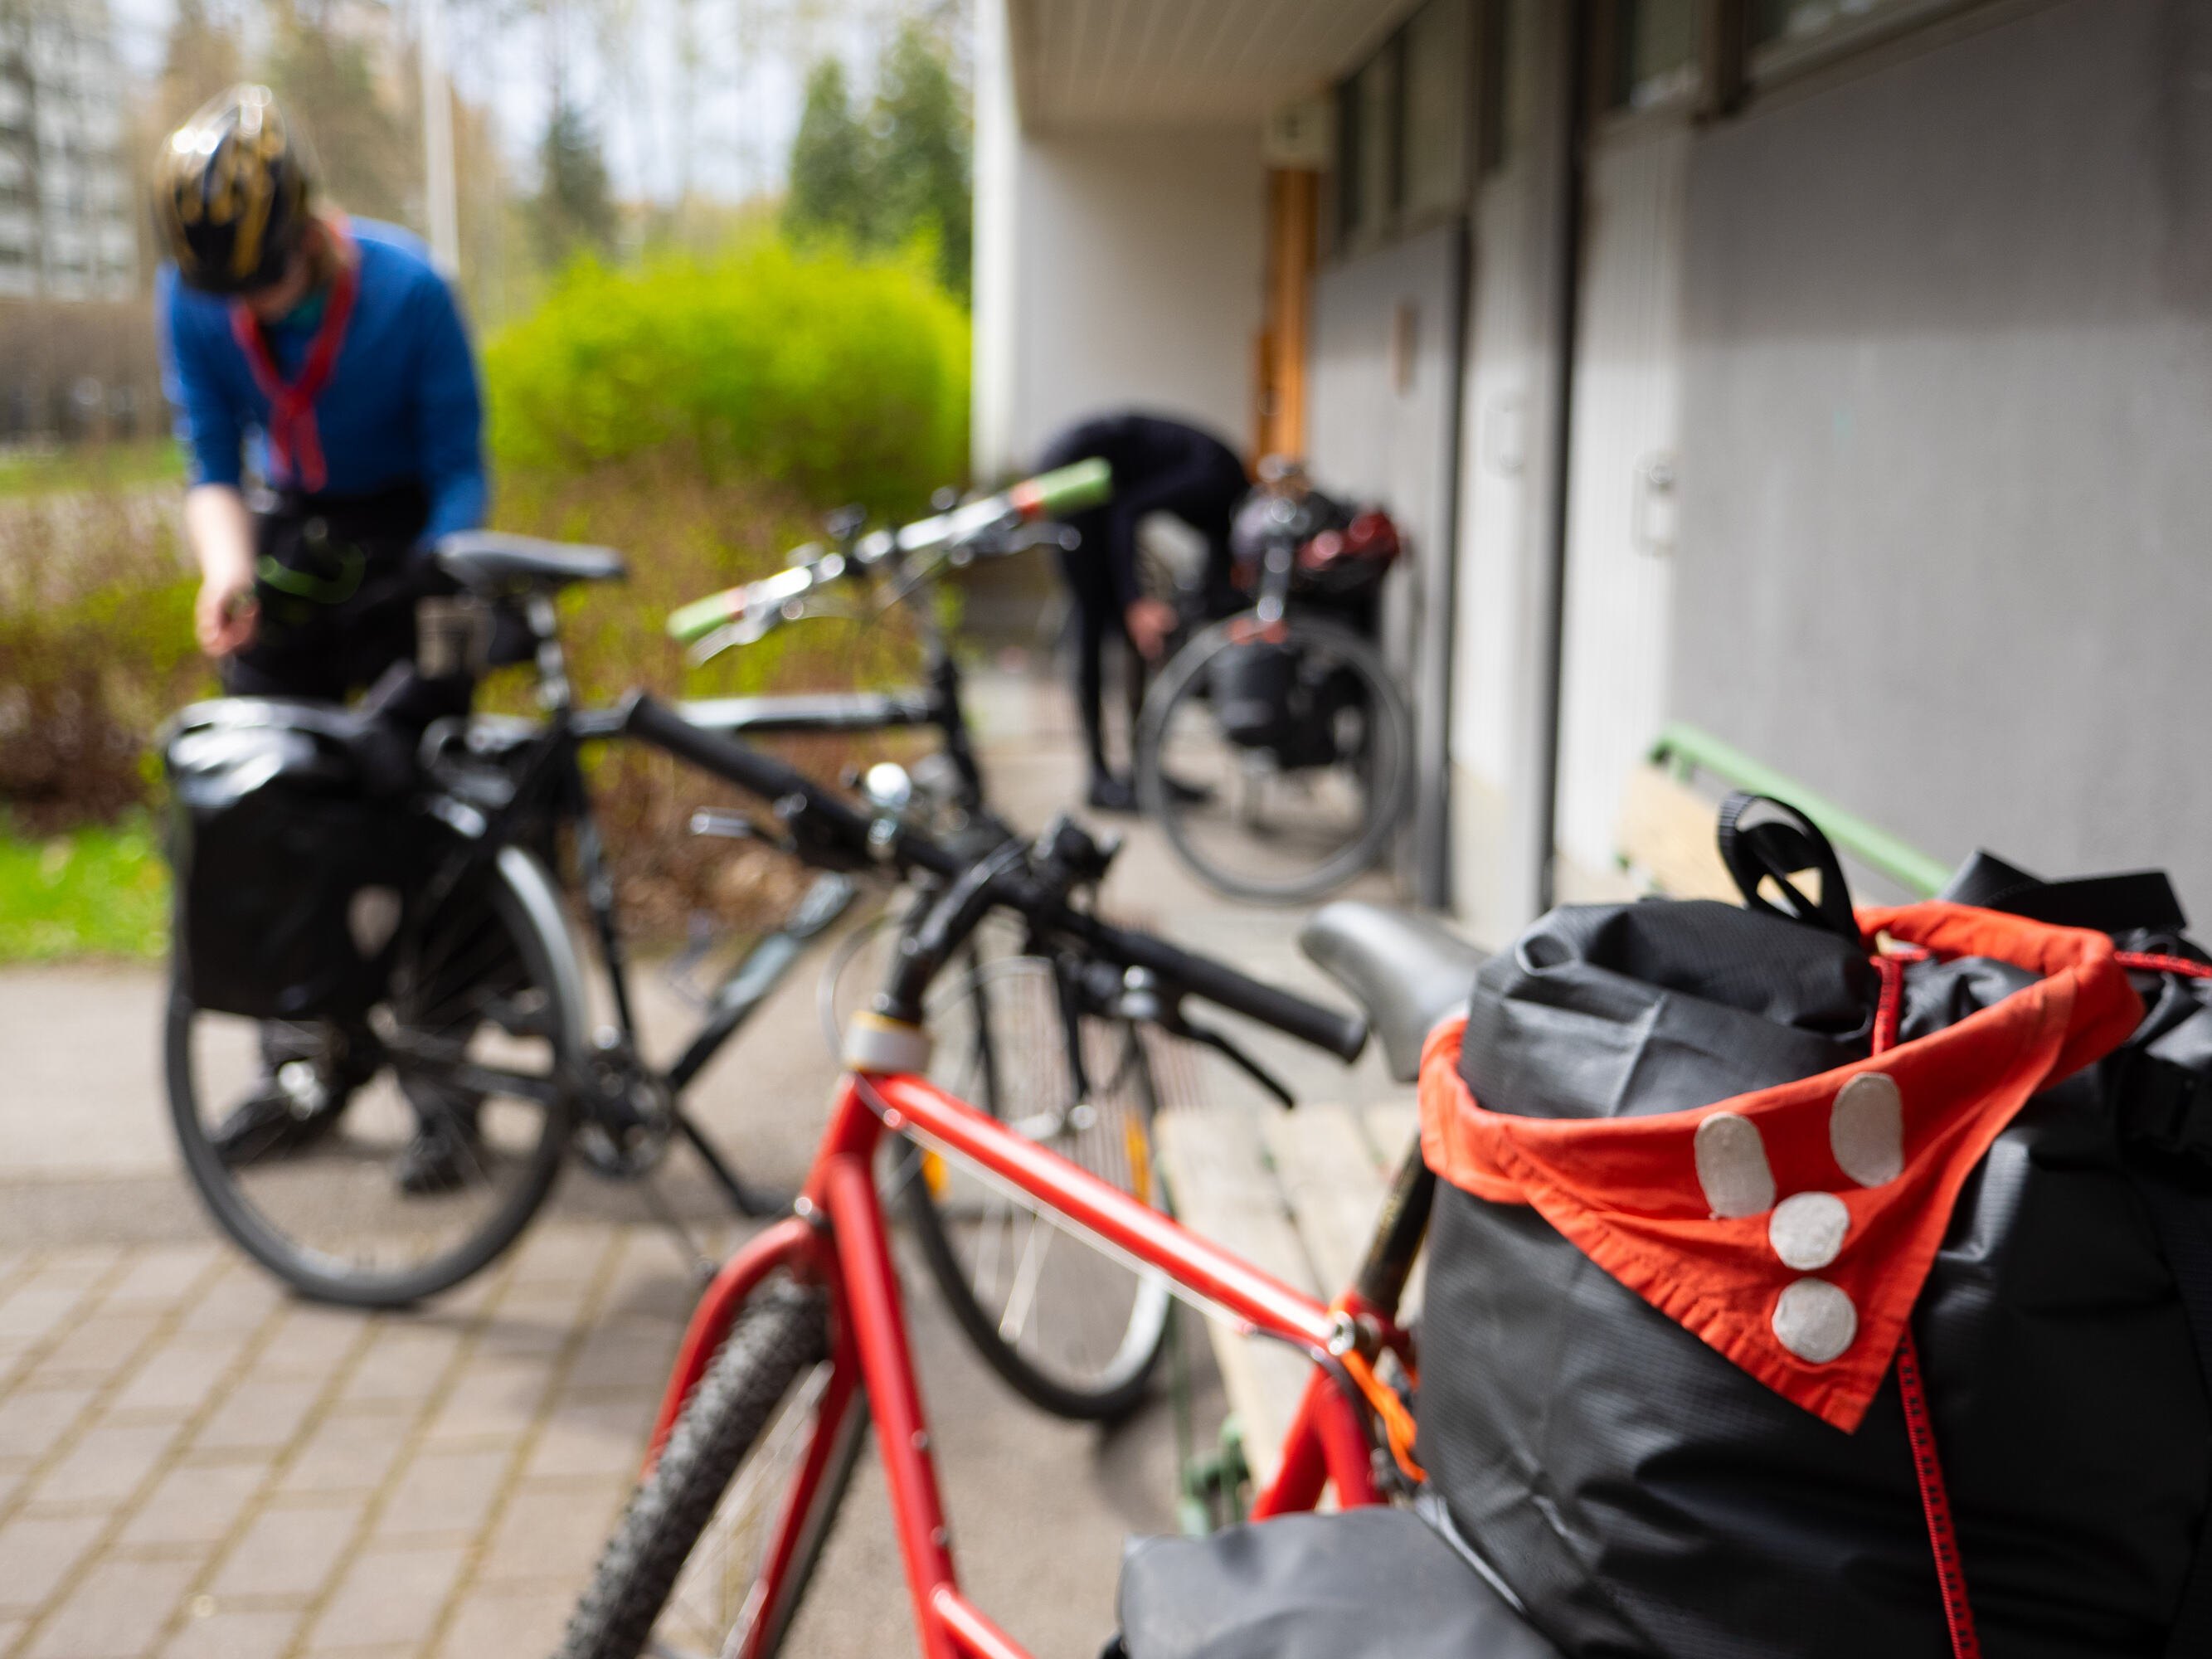
\includegraphics[width=\linewidth]{assets/pyörävaellus1}
	\captionof{figure}{Kolme rusakkoa lähti pyöräilemään KuRu:n
	varastolta länttä kohti torstaiaamuna 9.5. Ensimmäinen tekninen
	vika ilmestyi jo 600 metrin jälkeen, joka saatiin nopeasti korjattua.}
\end{Figure}

\begin{multicols}{2}
	\begin{Figure}
		\noindent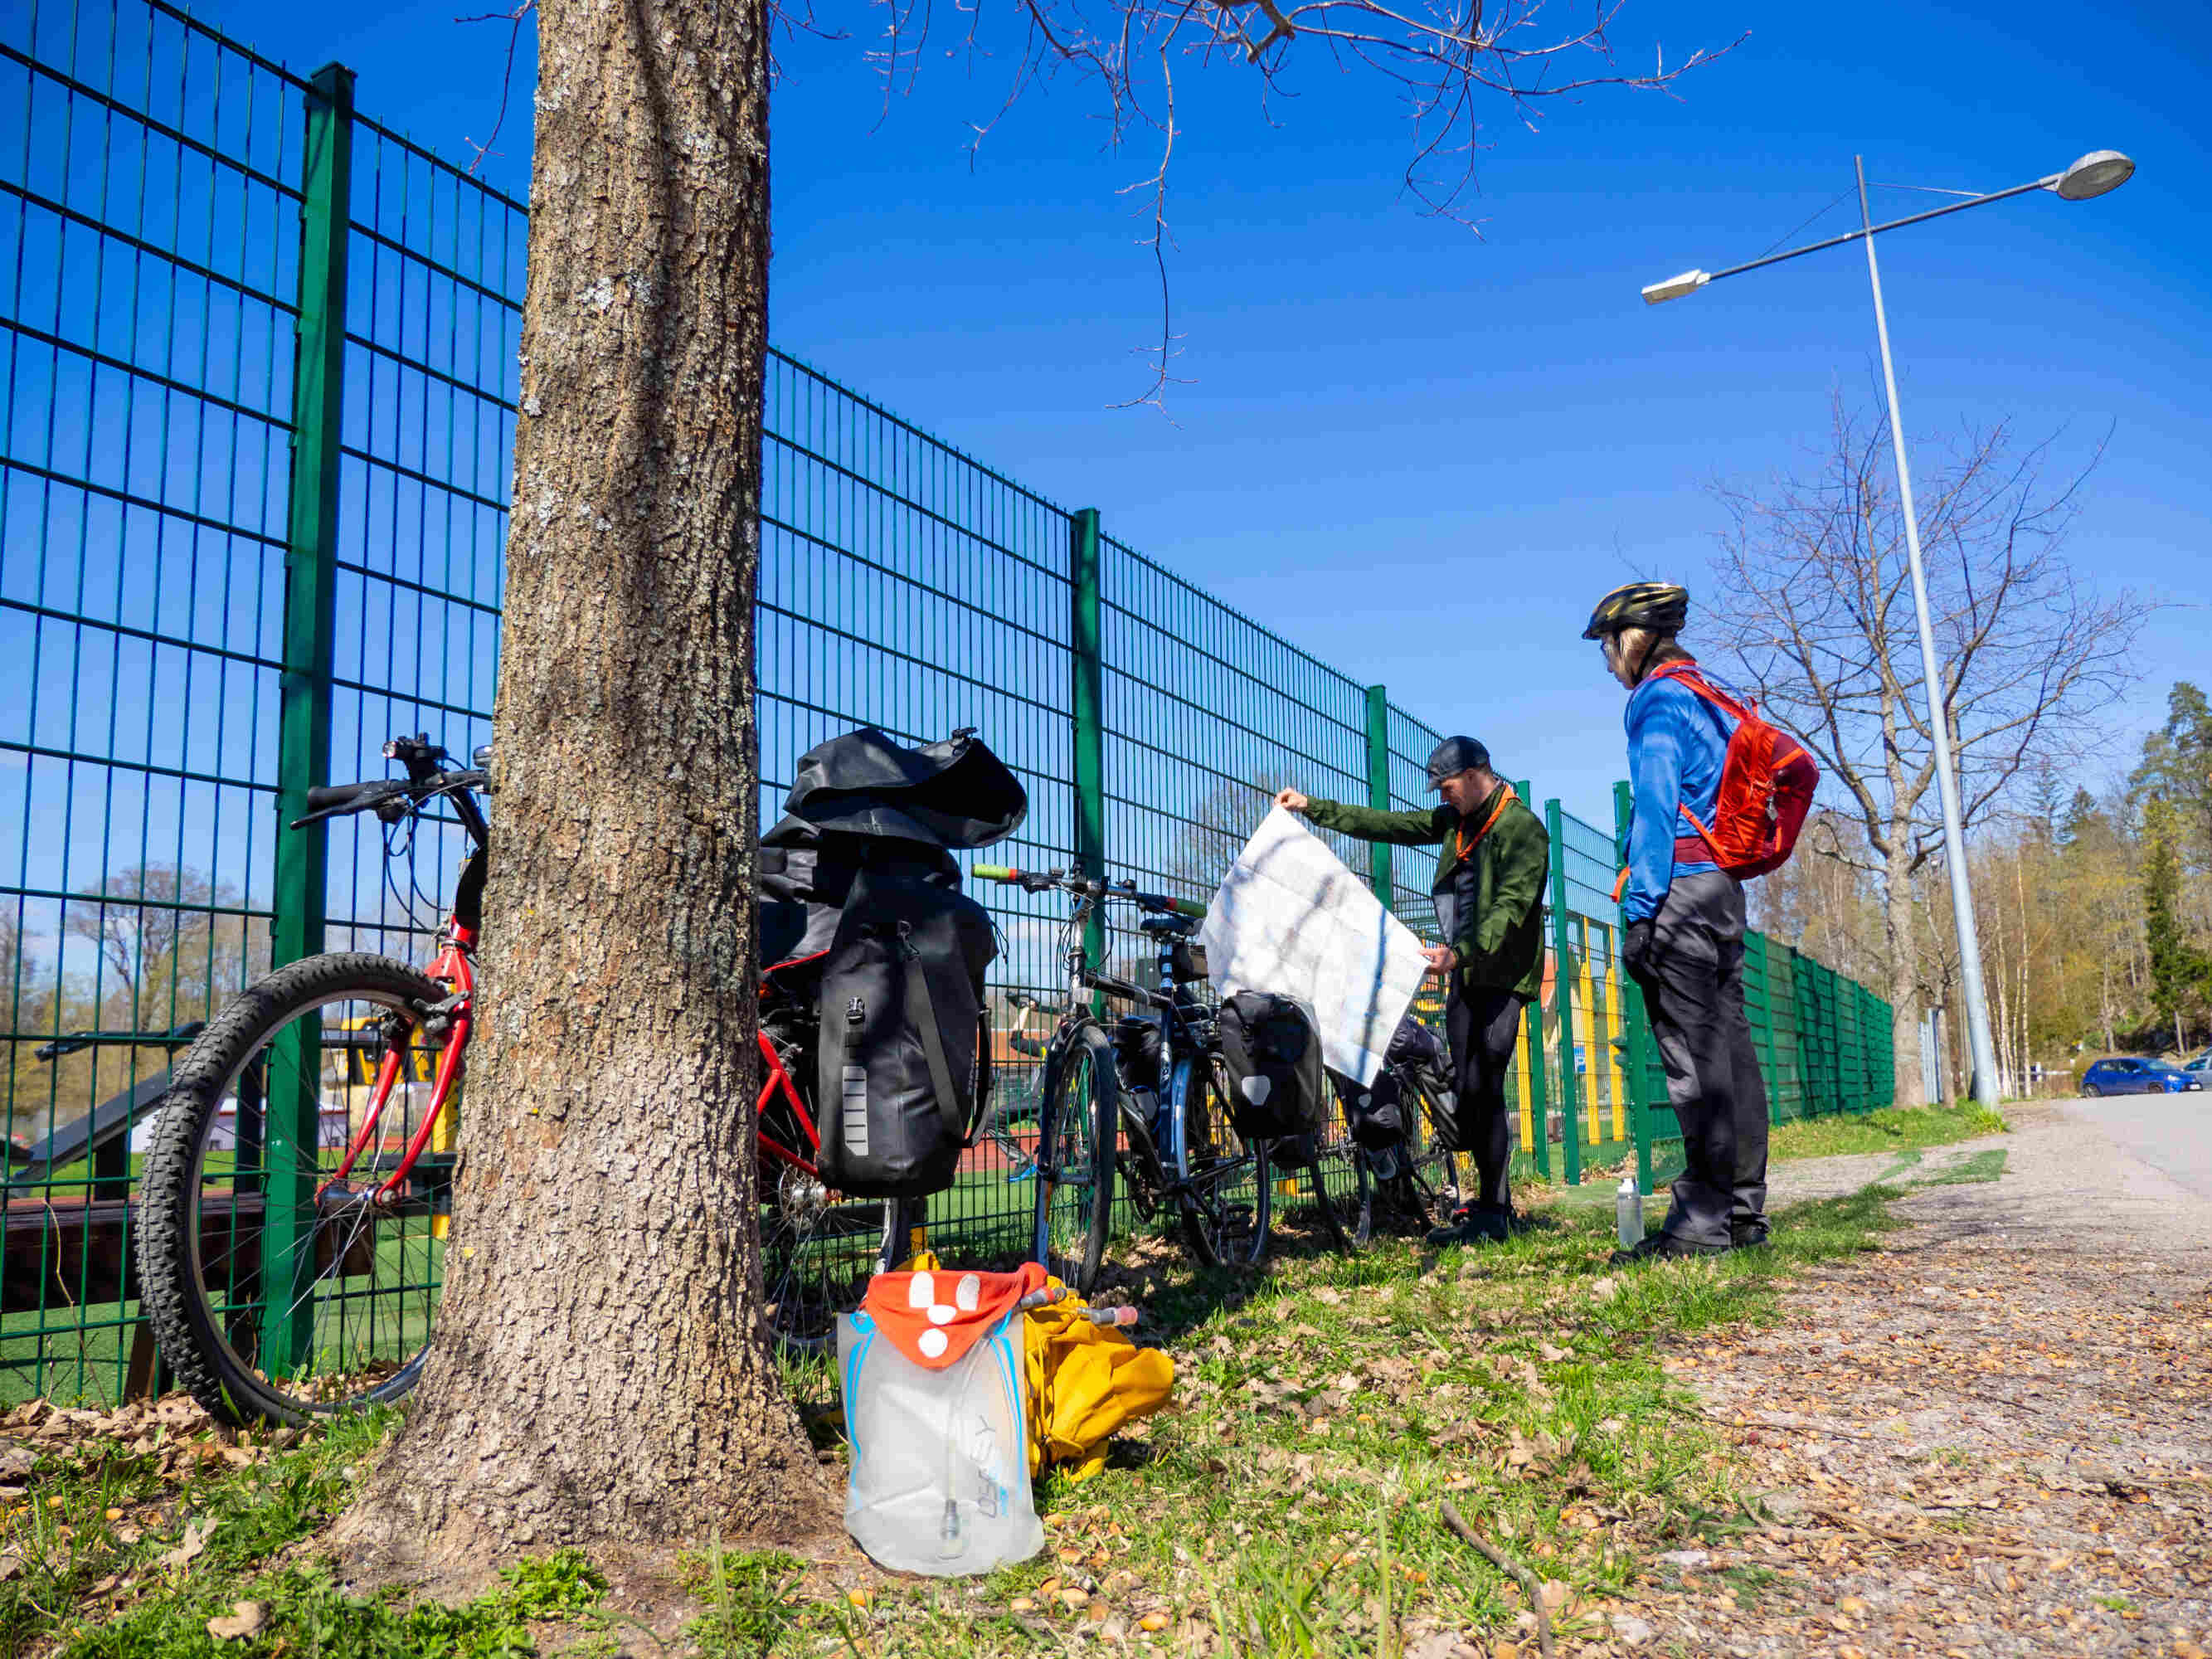
\includegraphics[width=\linewidth]{assets/pyörävaellus3}
		\captionof{figure}{Ensimmäiseksi lounaspaikaksi valittiin
		Kauklahden urheilukenttä, jonka jälkeen matka jatkui kohti Kirkkonummea.}
	\end{Figure}
	\columnbreak
	\begin{Figure}
		\noindent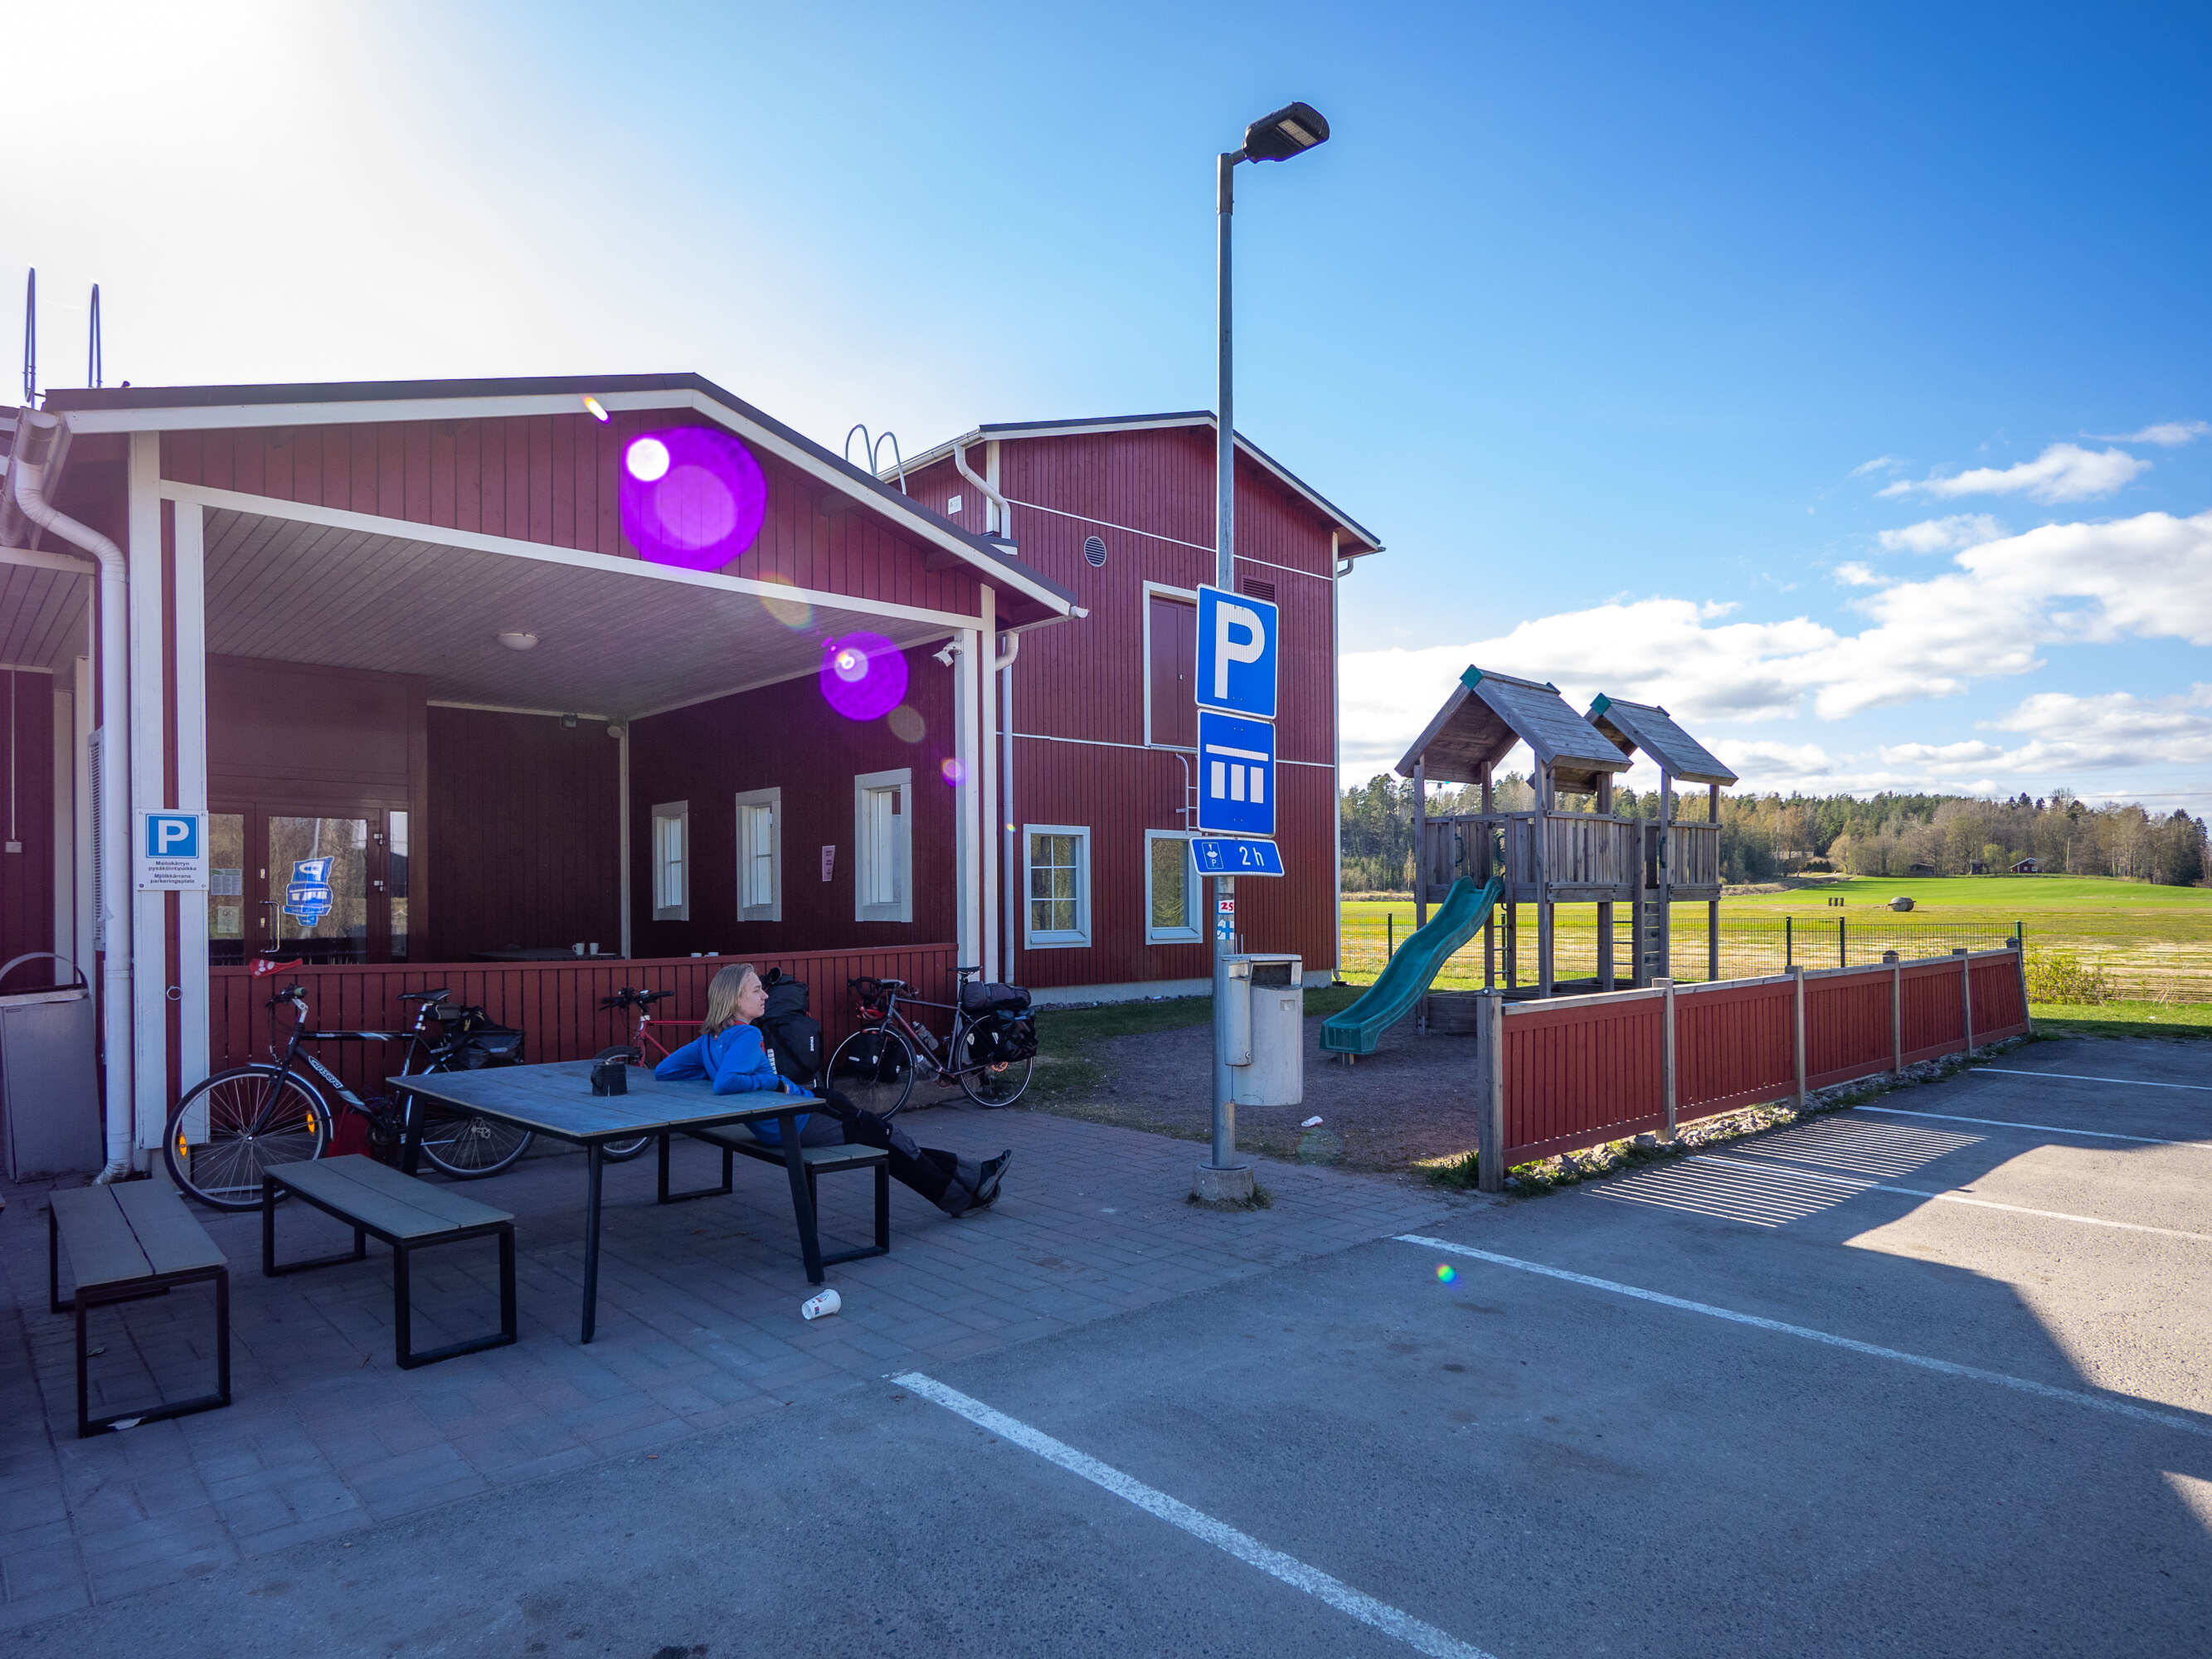
\includegraphics[width=\linewidth]{assets/pyörävaellus4}
		\captionof{figure}{Vaelluksen ensimmäinen jäätelö syötiin
		sitten Pickalan huoltoasemalla, noin 10~km meidän
		päämäärästämme.}
	\end{Figure}
\end{multicols}

\begin{Figure}
	\noindent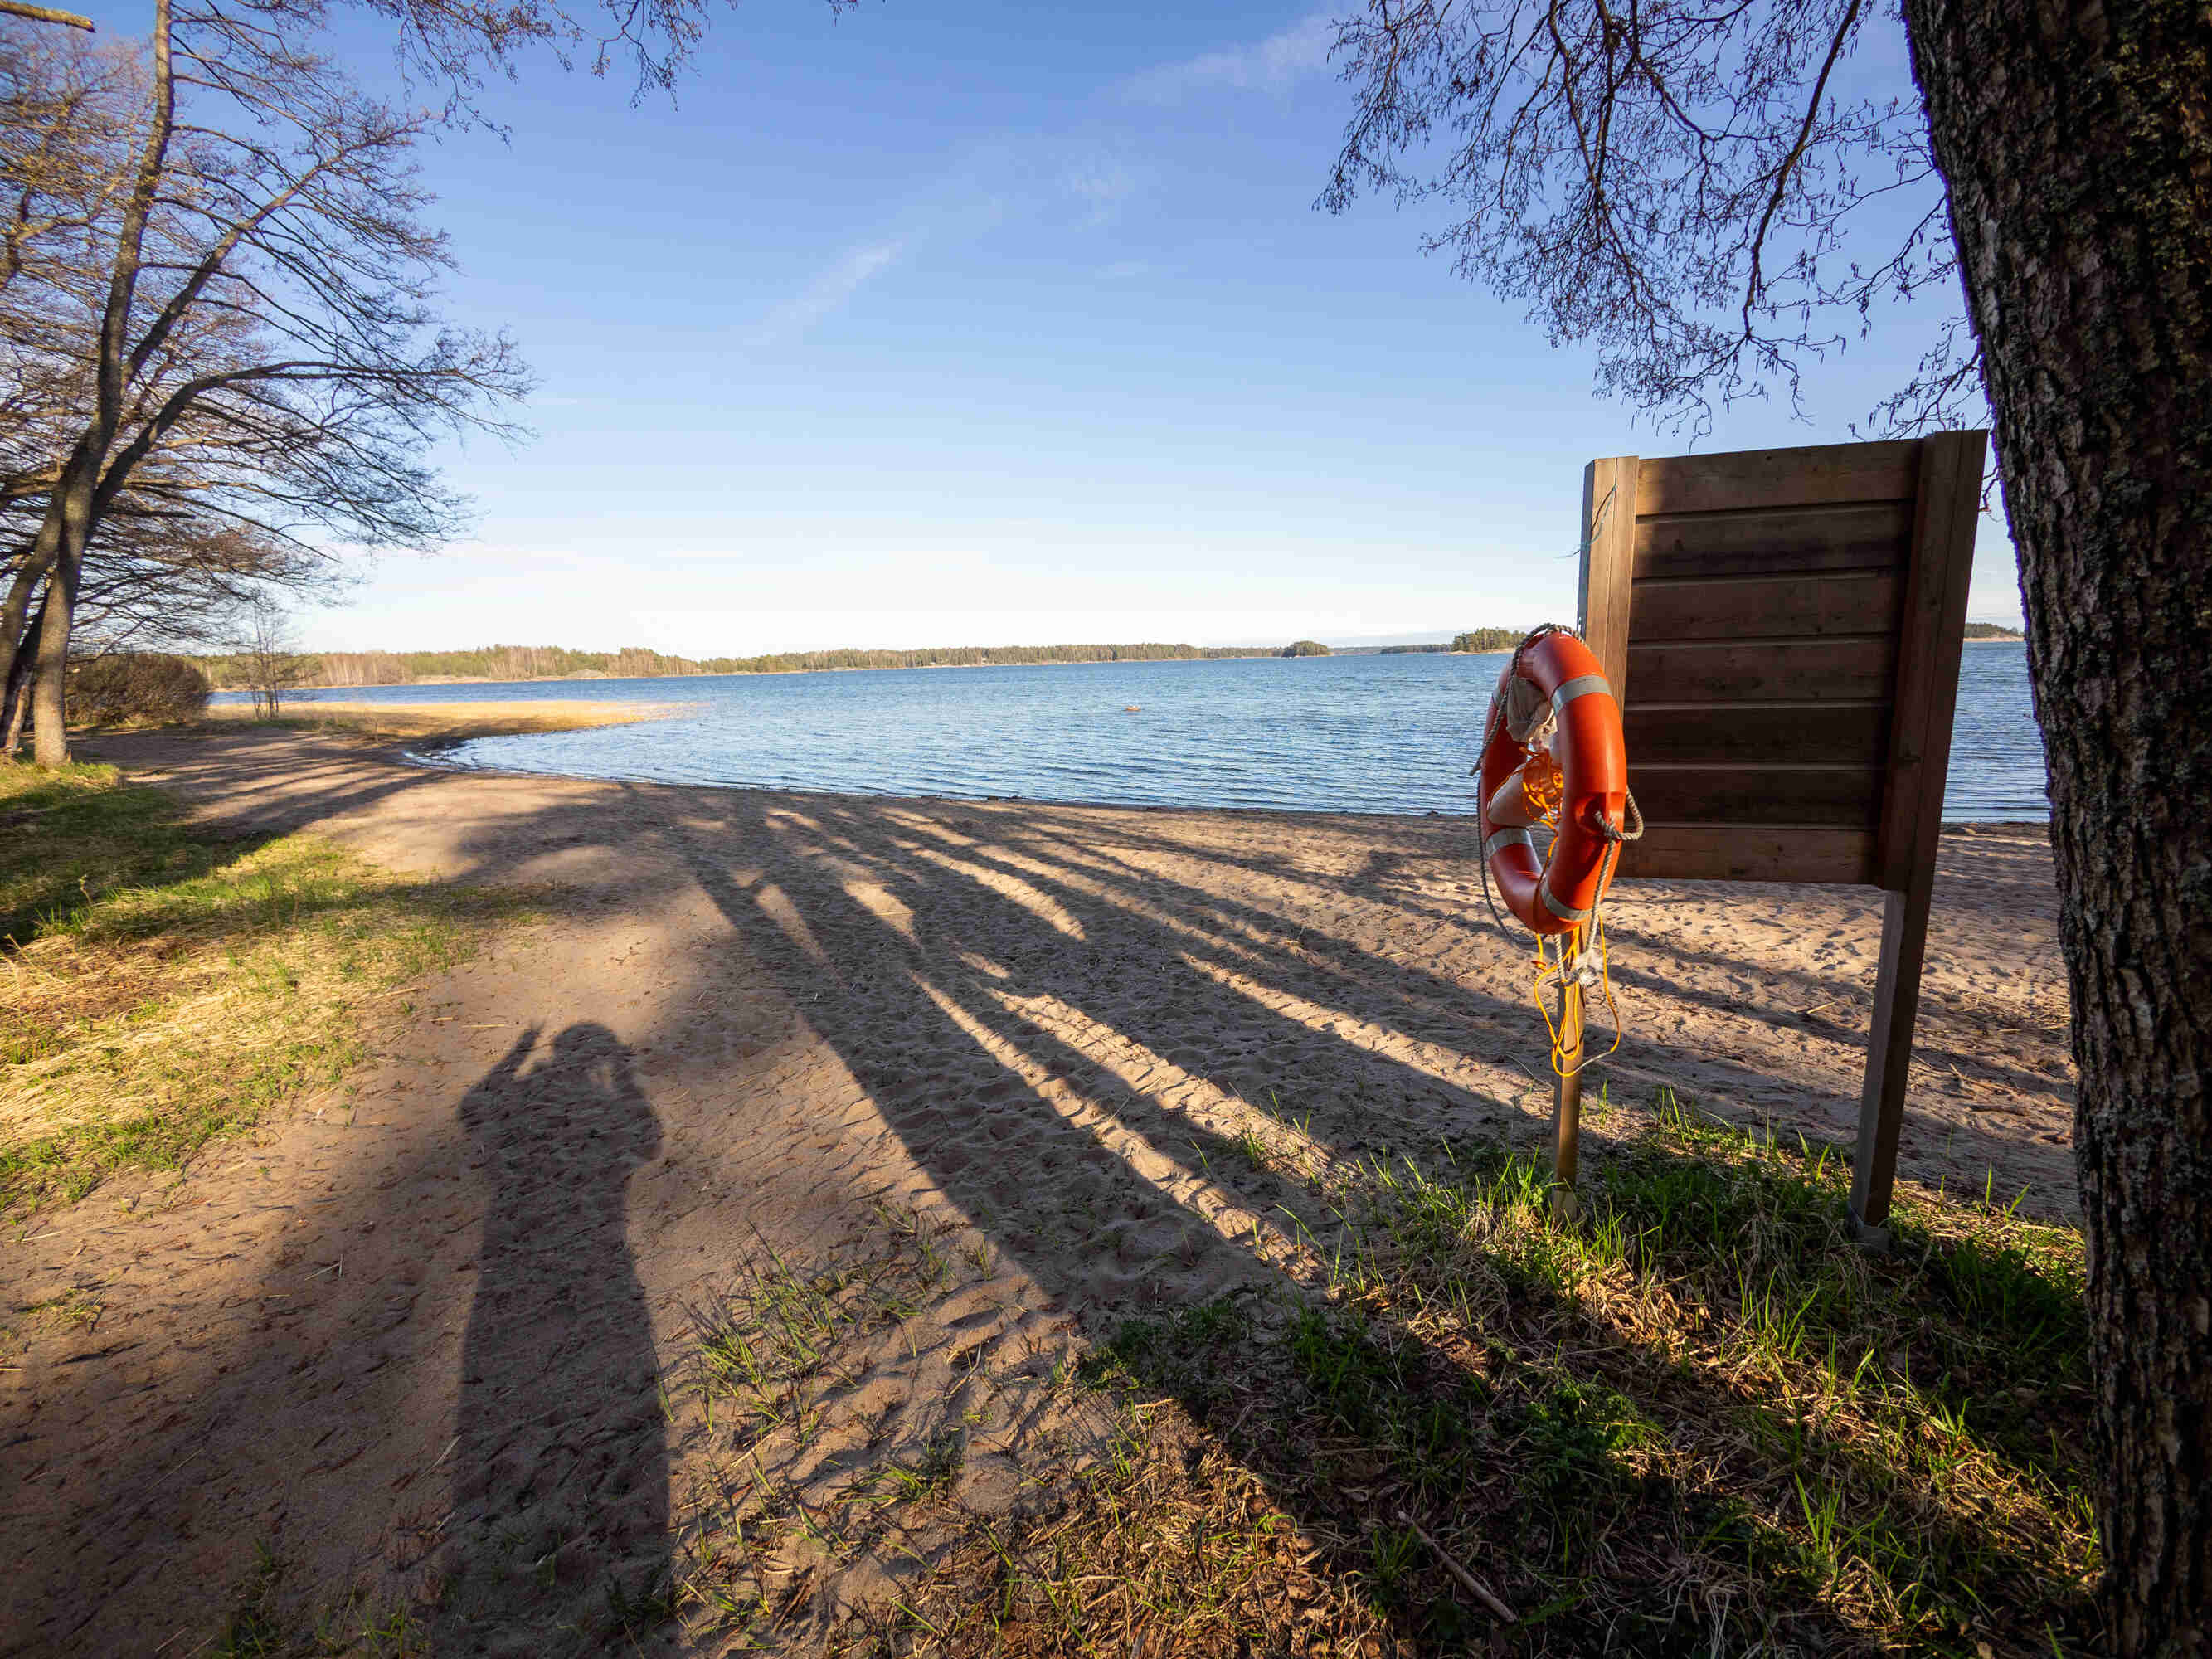
\includegraphics[width=\linewidth]{assets/pyörävaellus5}
	\captionof{figure}{Lyhyt mutta stressaava Inkoon Rannikkotien
	pätkä odotti meitä, jota seurasi rennompi mutta kuoppainen
	hiekkatie -- ja vihdoin löytyi meidän yöpymispaikka: Kopparnäs,
	Inkoo.}
\end{Figure}

\begin{multicols}{2}
	\begin{Figure}
		\noindent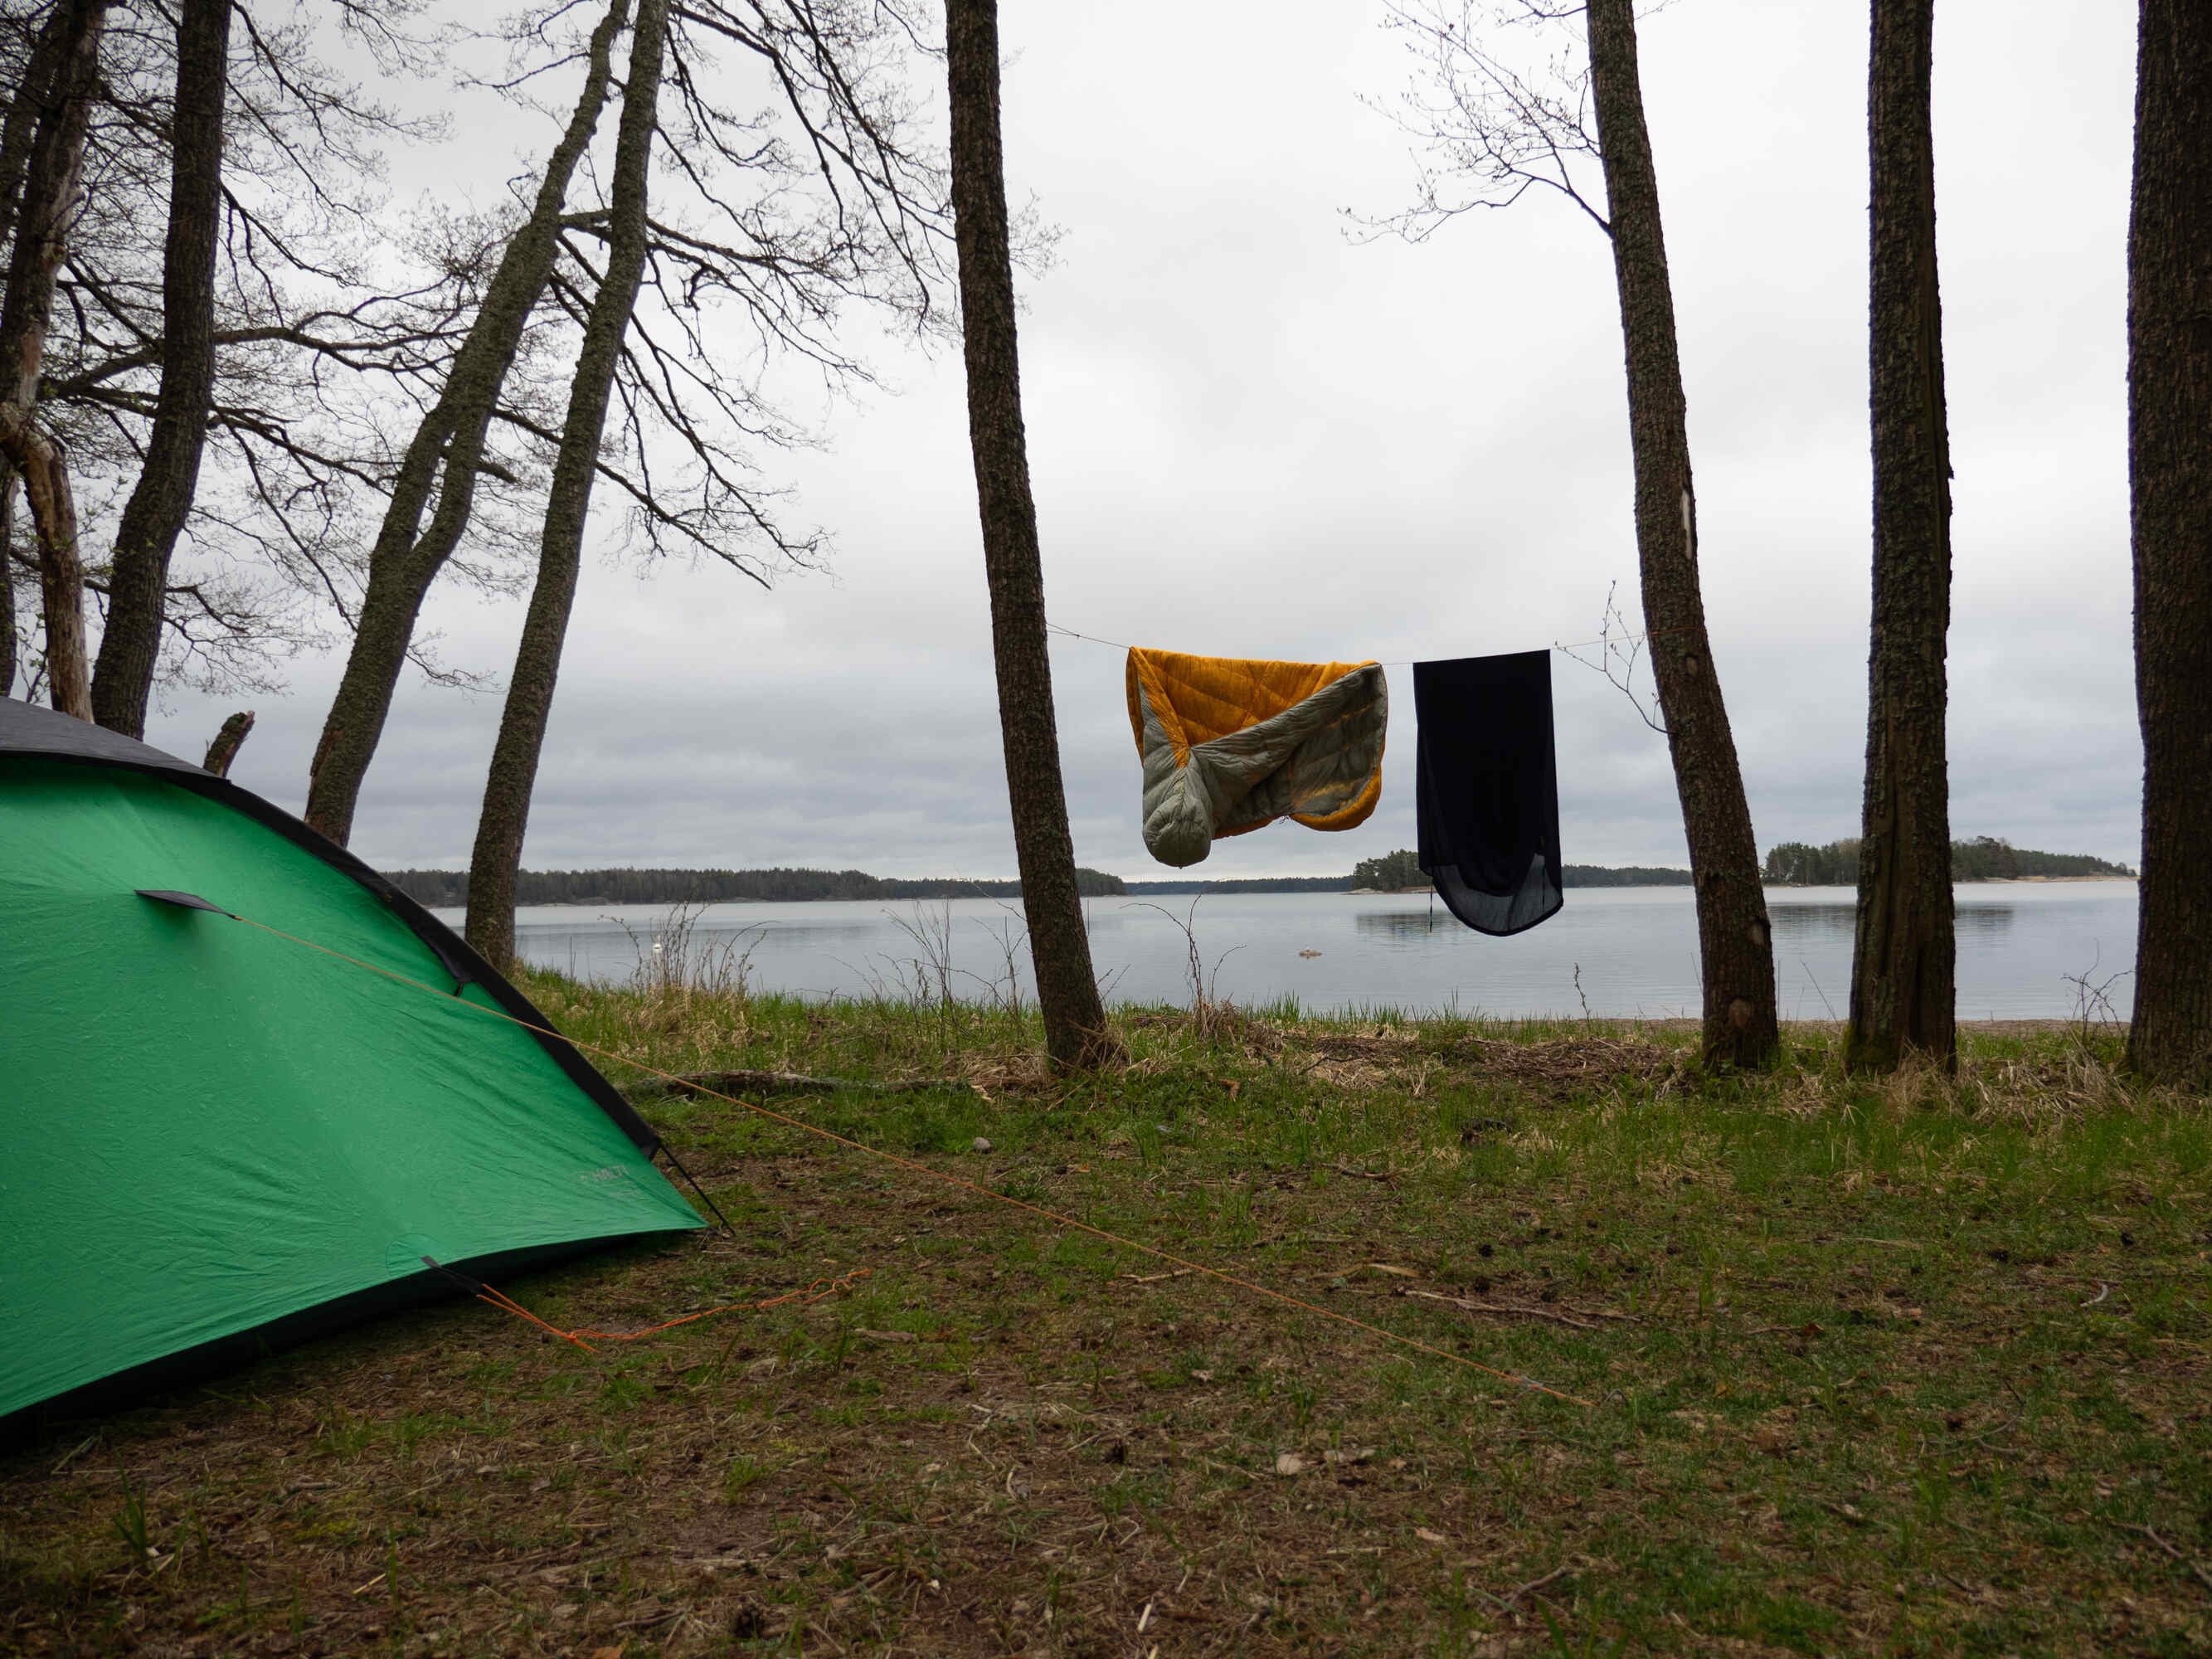
\includegraphics[width=\linewidth]{assets/pyörävaellus6}
		\captionof{figure}{74~km jälkeen jotkut rusakoista alkoivat
		tuntea \textbf{vähän} kipua ja \textbf{vähän} väsymystä.
		Äänekkäät kalatiirat rannalla uhkasivat olla antamatta meidän
		nukkua, mutta onneksi lähtivät illallisen jälkeen. Sade saapui
		yöllä, mutta kiltisti lähti ennen herätystä.}
	\end{Figure}
	\columnbreak
	\begin{Figure}
		\noindent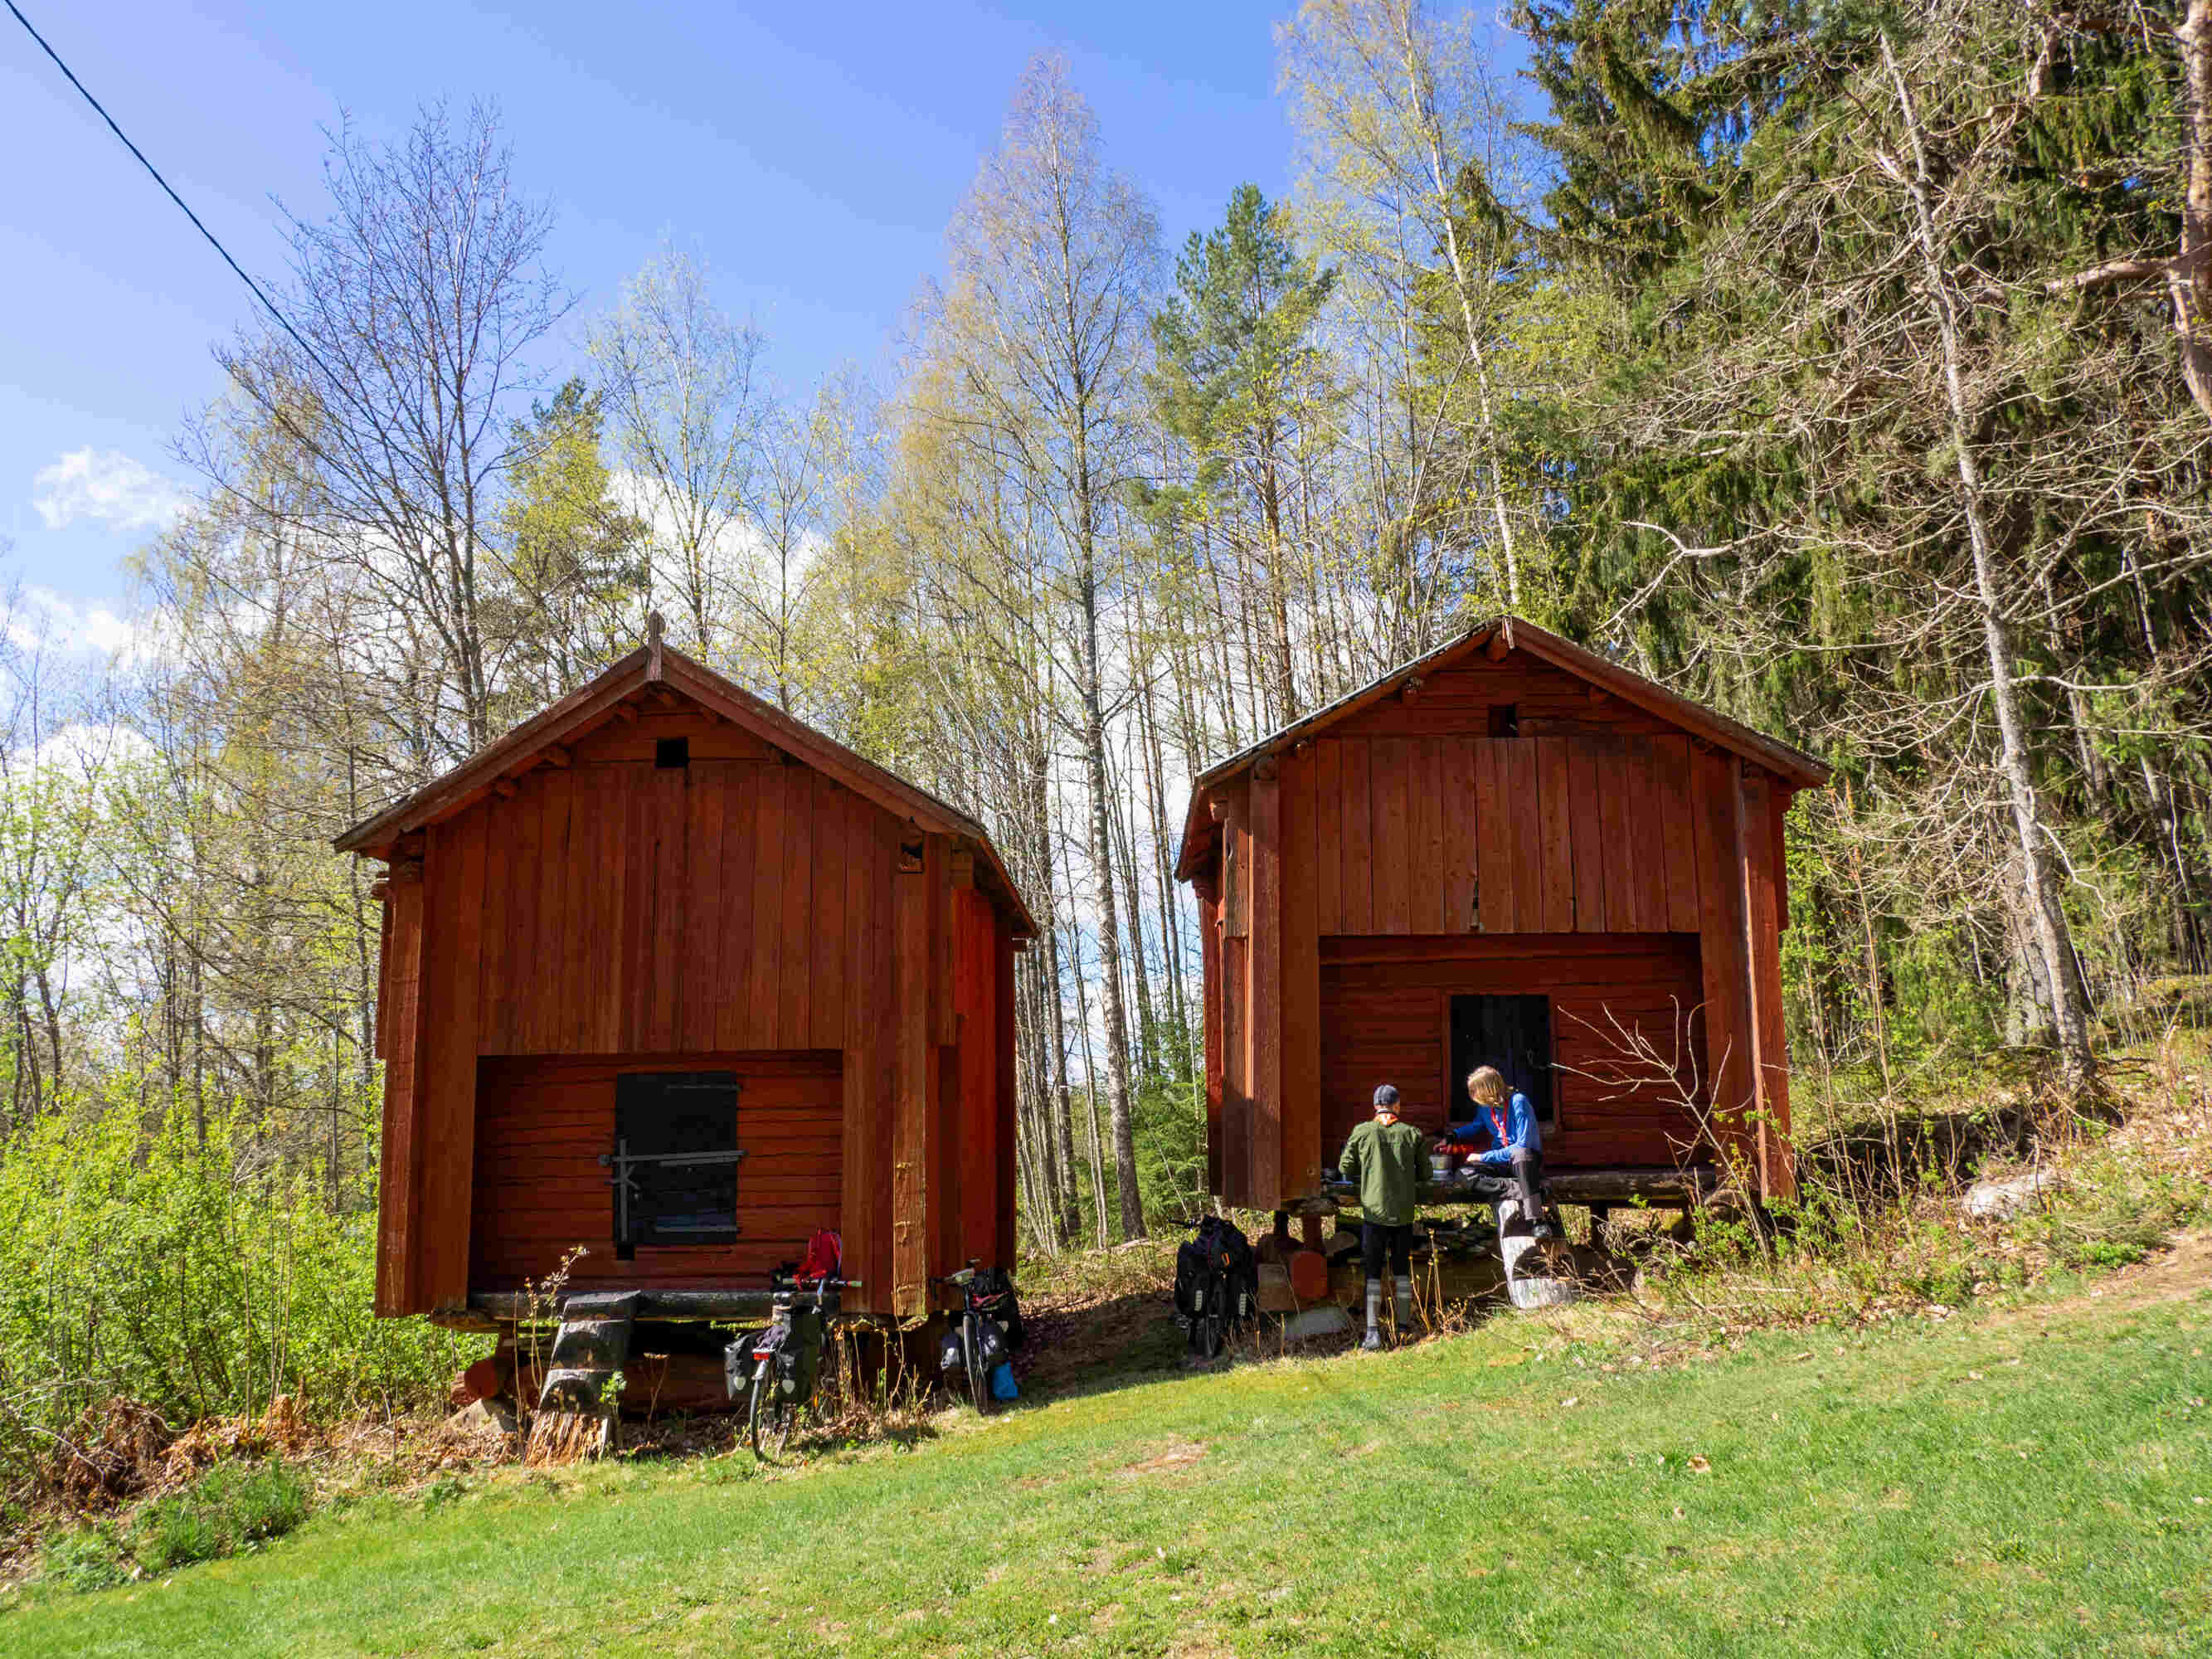
\includegraphics[width=\linewidth]{assets/pyörävaellus7}
		\captionof{figure}{Toinen päivä toi meidät pohjoiseen, päämääränämme Lohja.
		Lounas syötiin noin puolivälissä, Siuntion kotiseutumuseossa.}
	\end{Figure}
\end{multicols}


\begin{Figure}
\begin{center}
	\noindent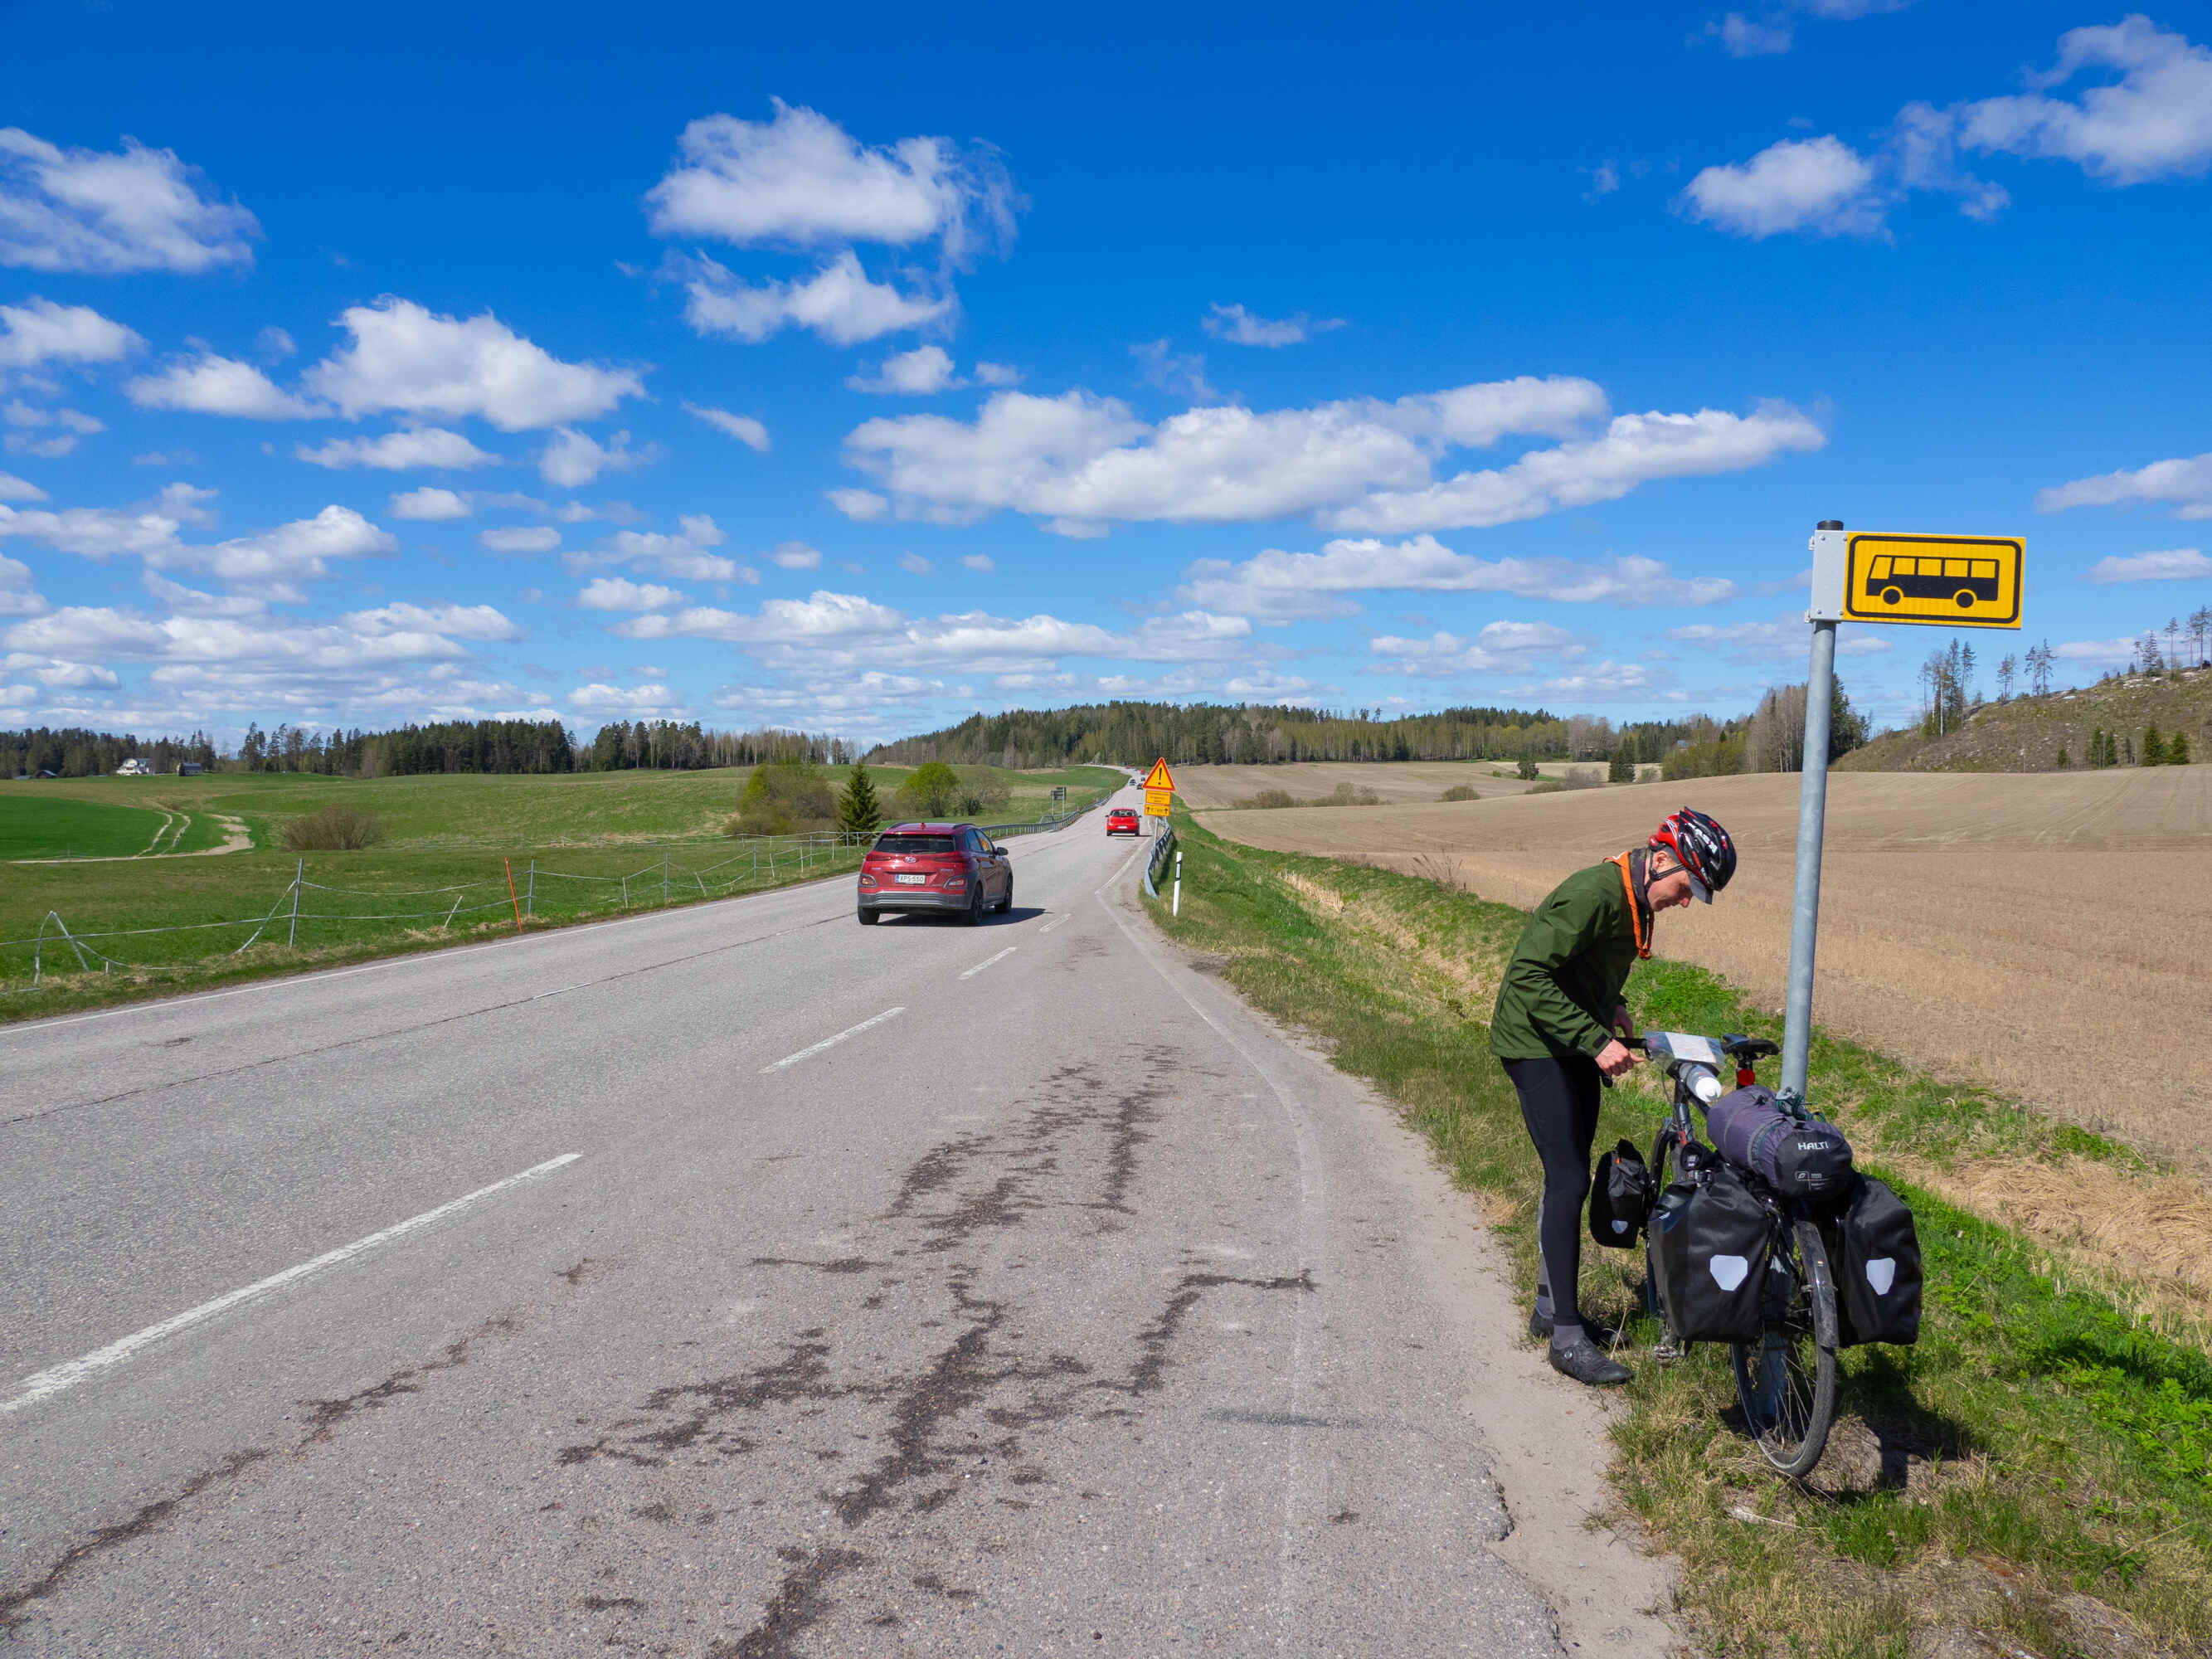
\includegraphics[width=0.90\linewidth]{assets/pyörävaellus8}
	\captionof{figure}{Matka jatkui hyvässä säässä.}
\end{center}
\end{Figure}
\begin{Figure}
\begin{center}
	\noindent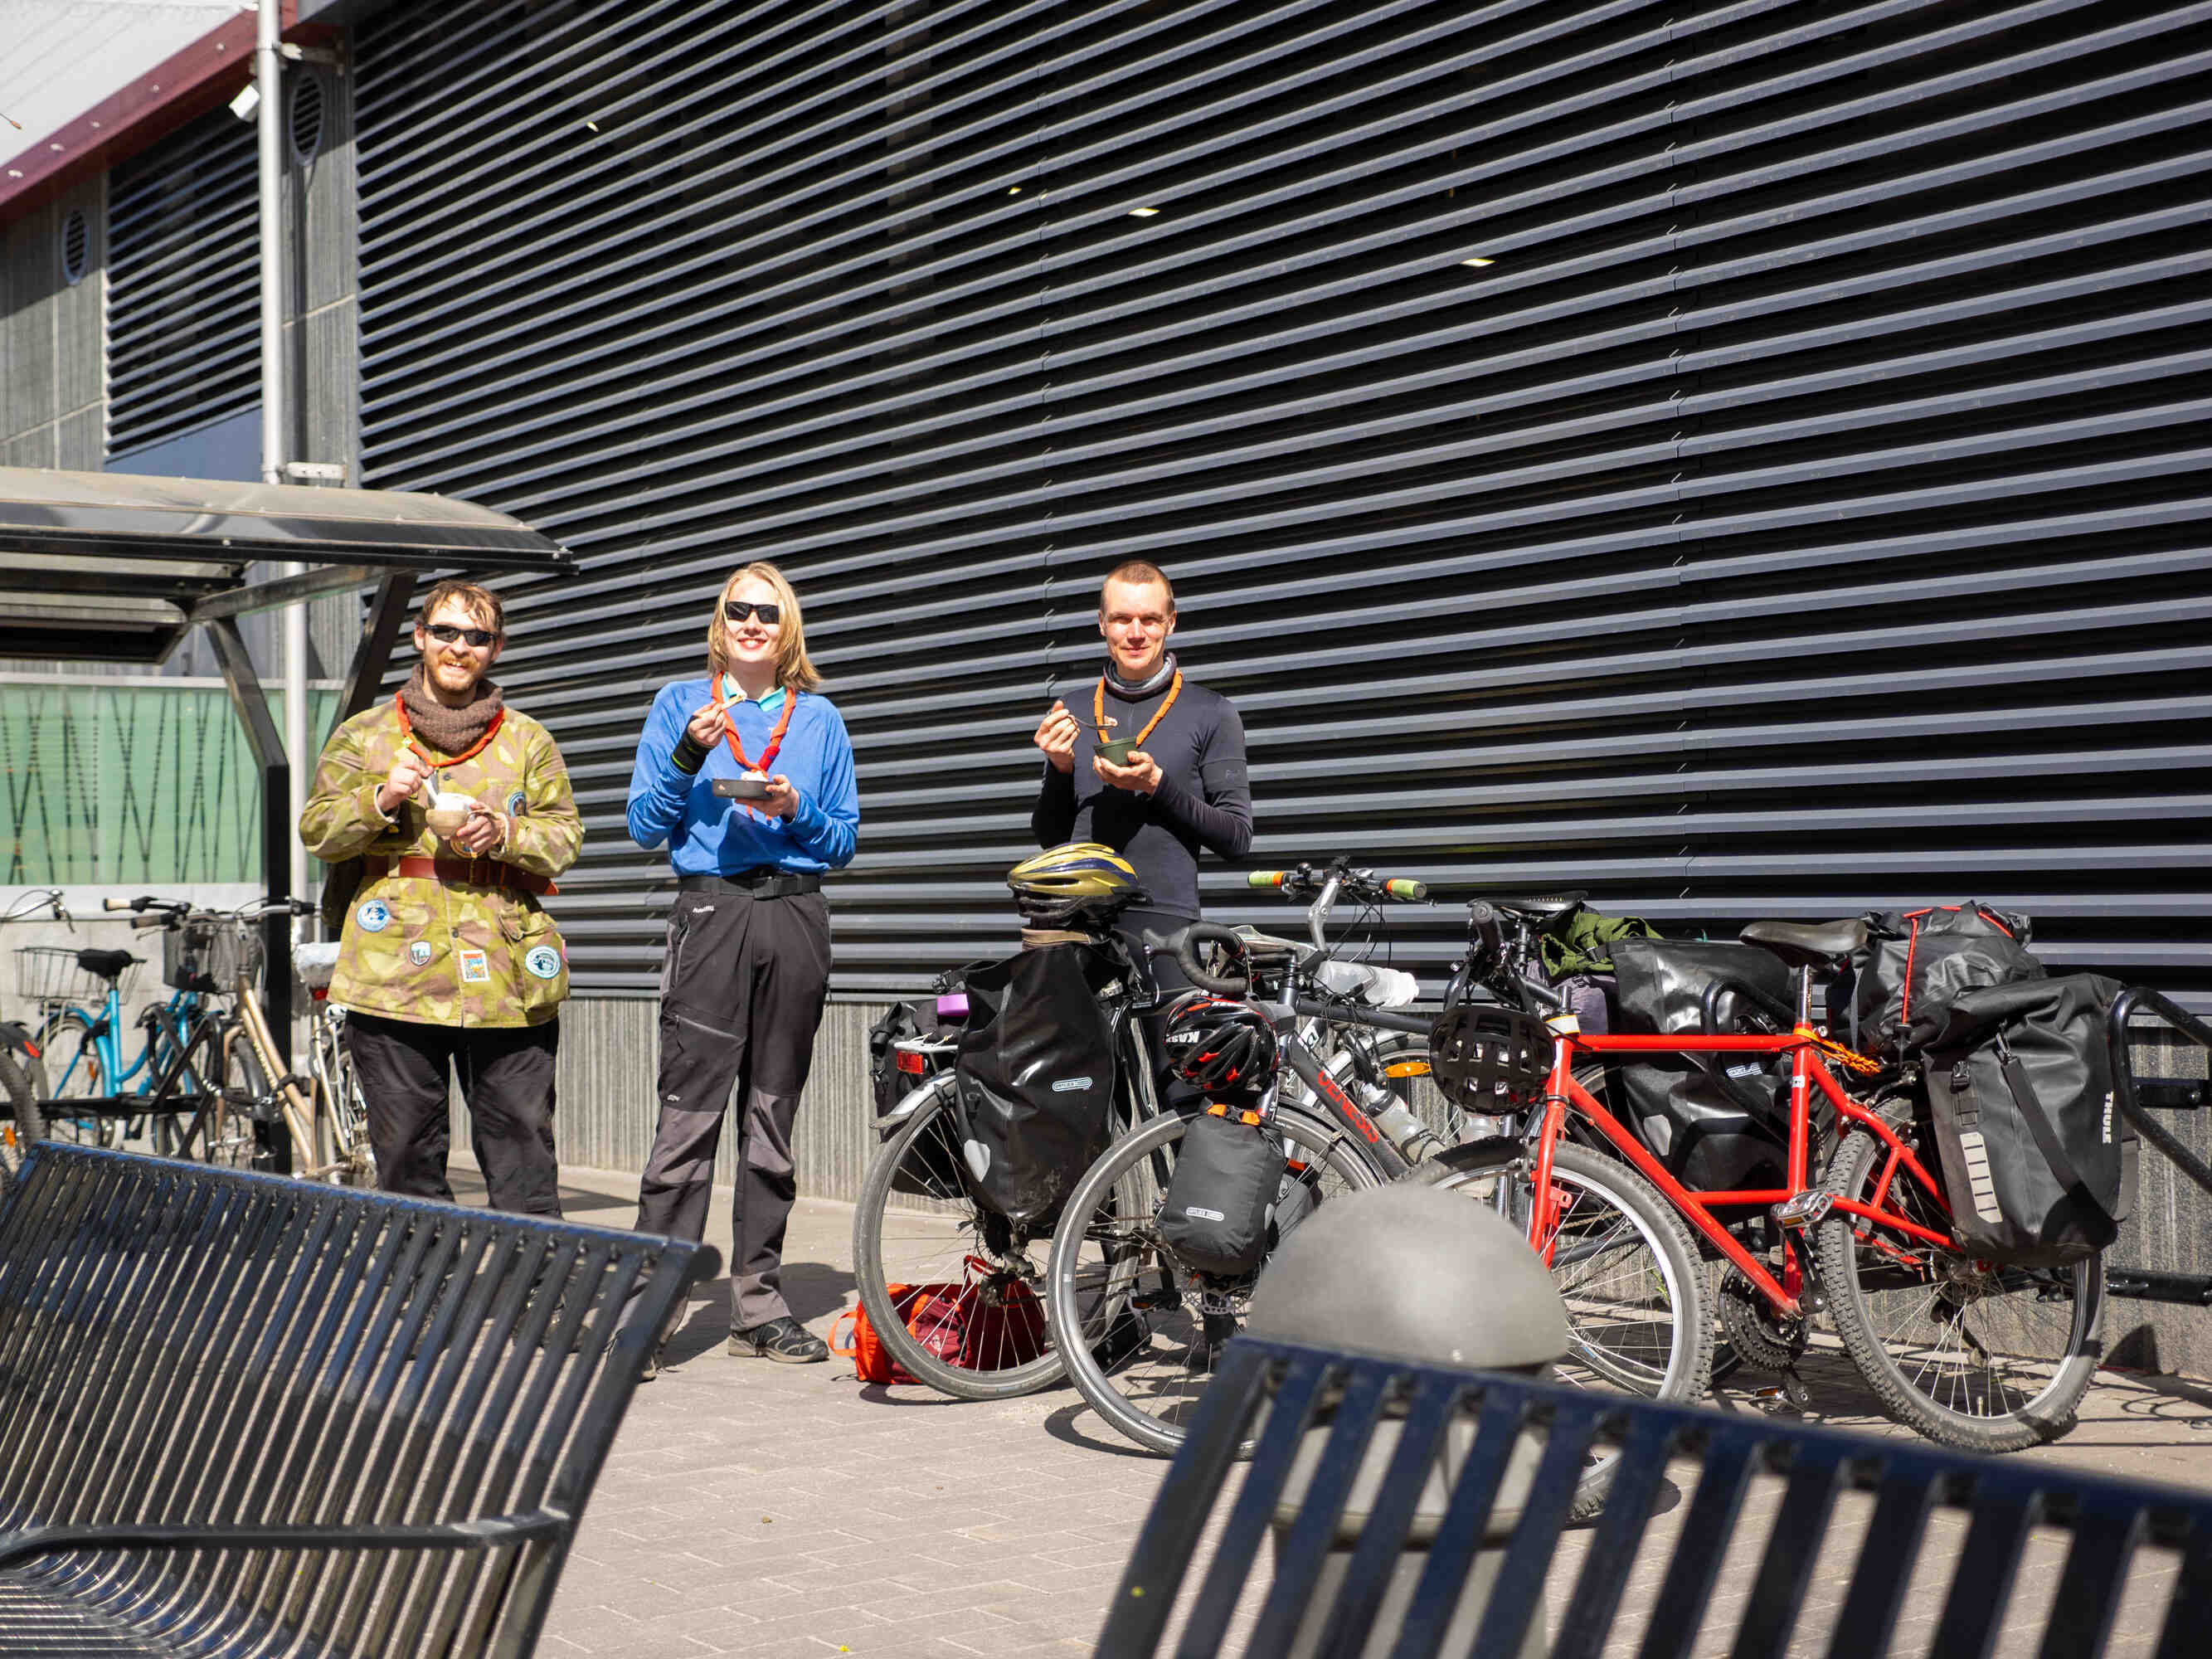
\includegraphics[width=0.90\linewidth]{assets/pyörävaellus9}
	\captionof{figure}{Lohjalla syötiin vaelluksen toinen jäätelö.}
\end{center}
\end{Figure}


\begin{Figure}
\begin{center}
	\begin{multicols}{2}
		\begin{center}
			\noindent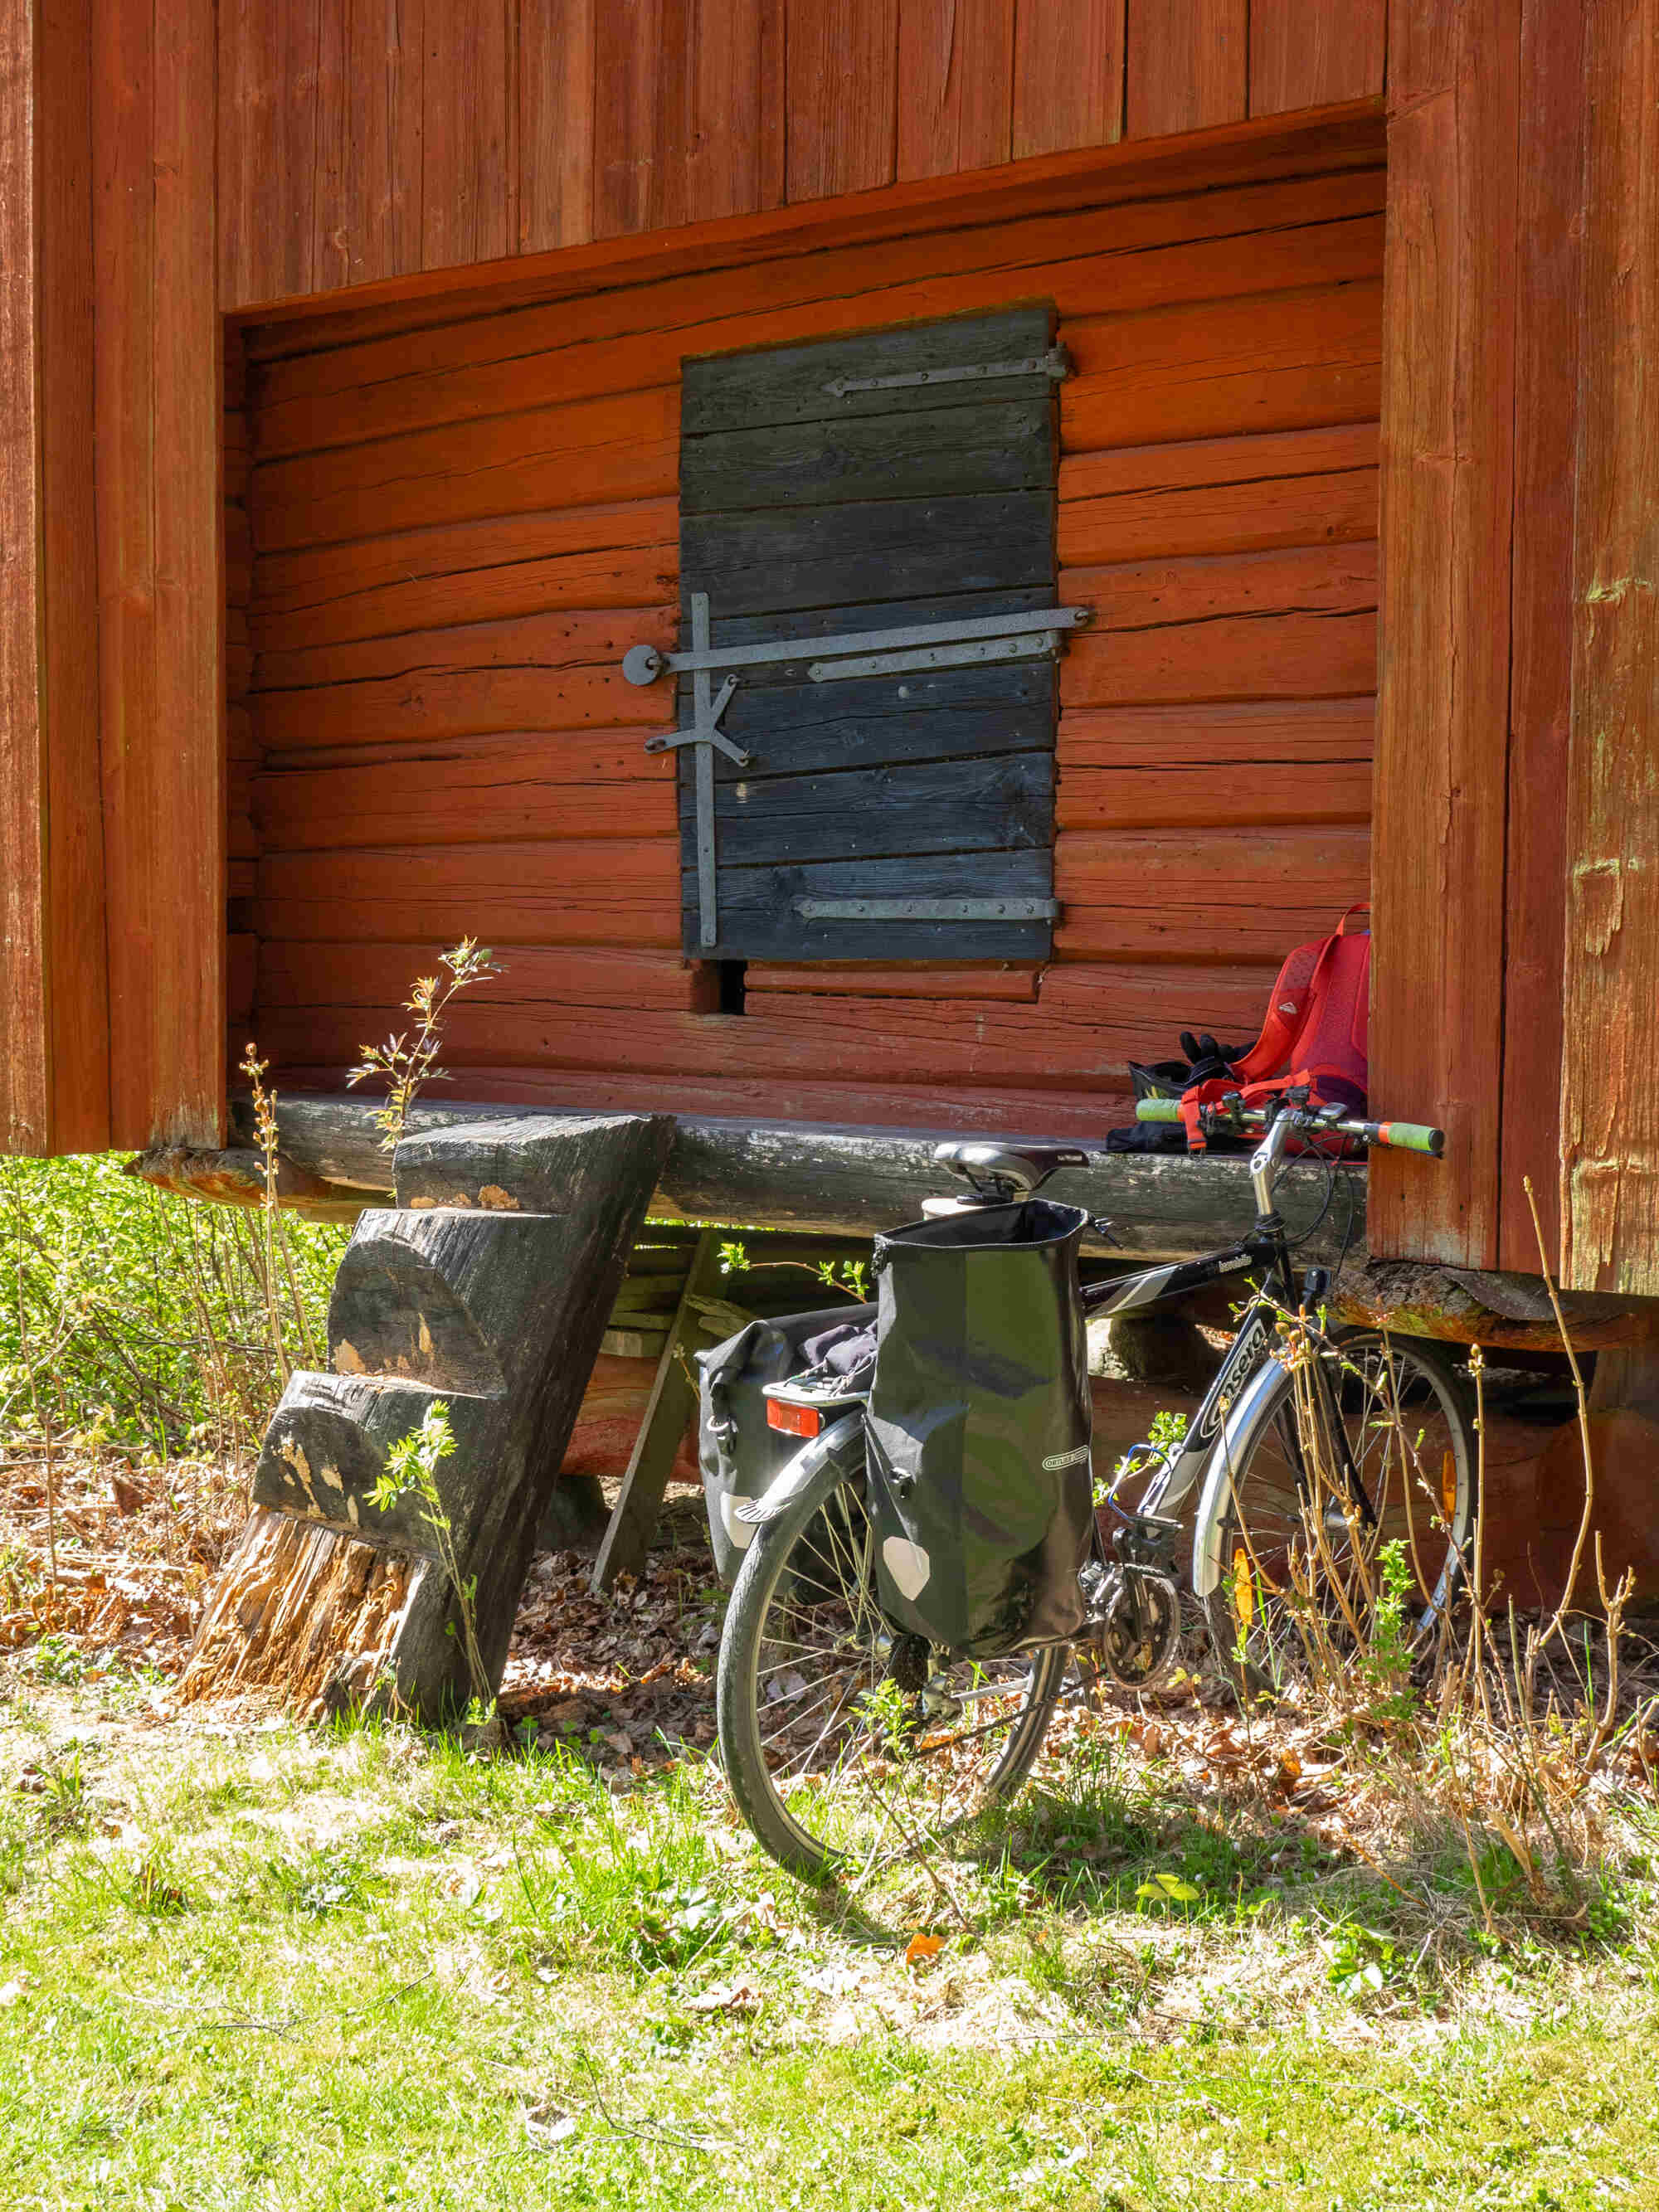
\includegraphics[width=1.05\linewidth]{assets/pyörävaellus10}
			\noindent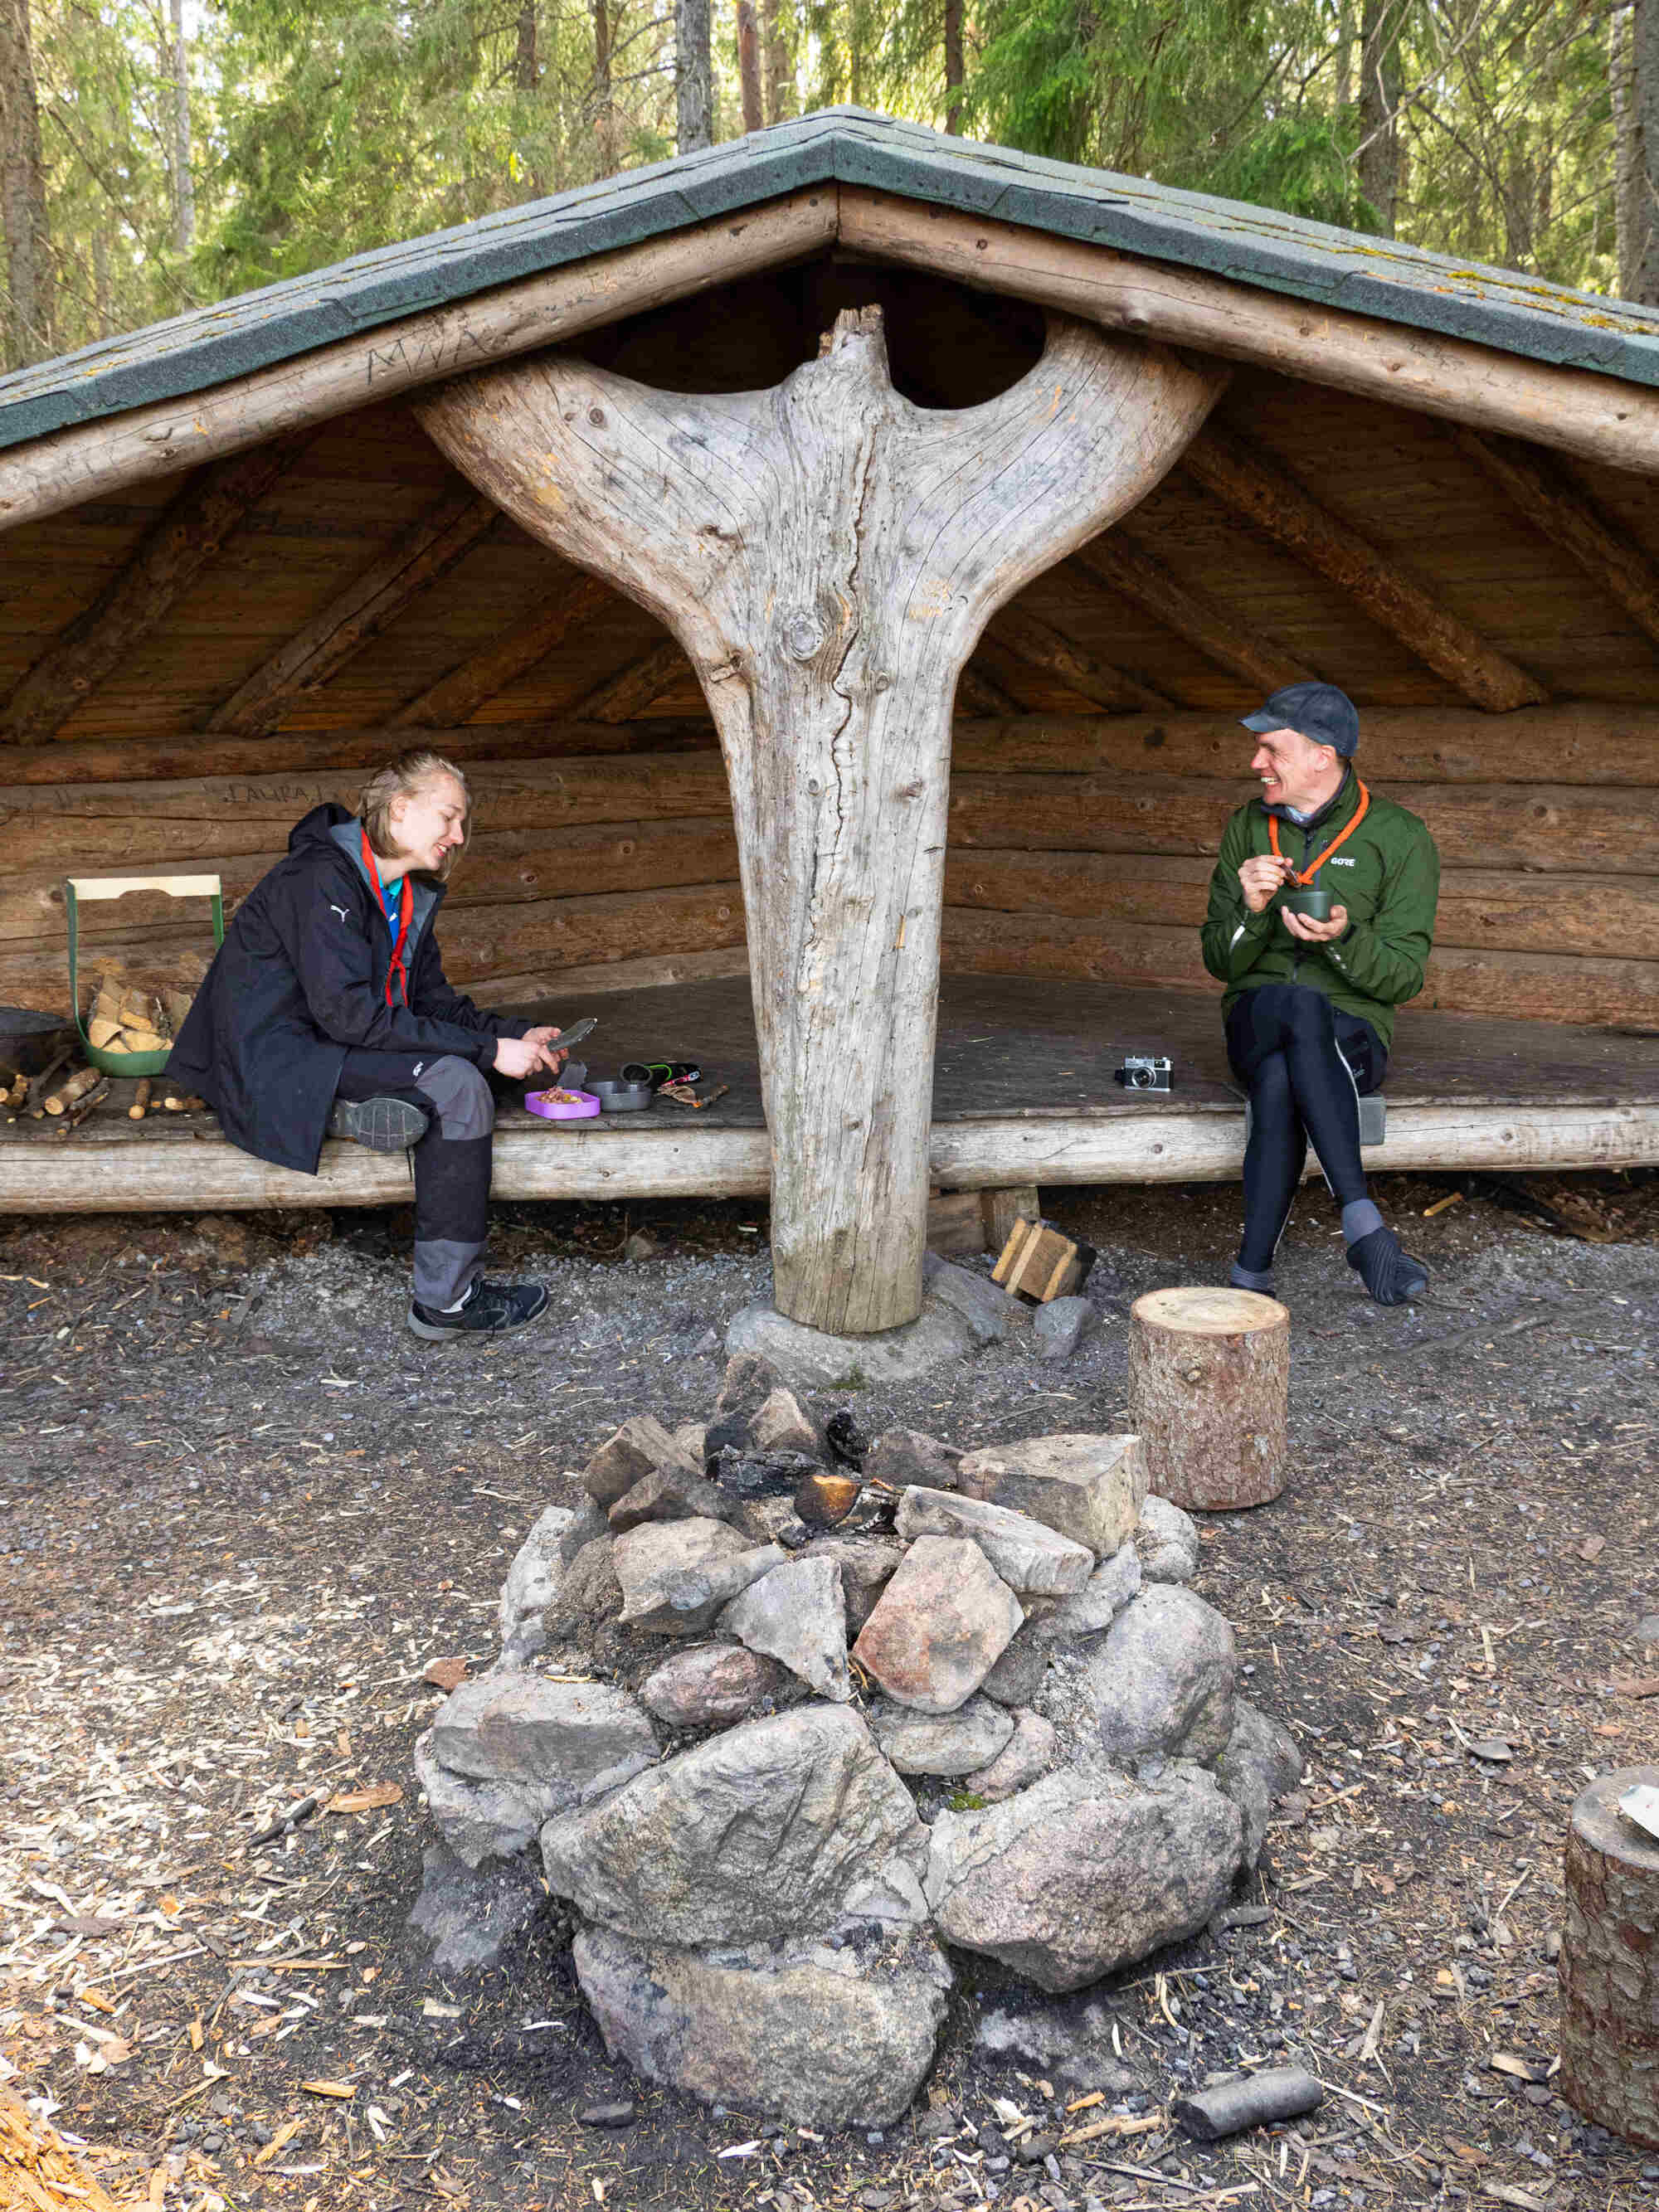
\includegraphics[width=1.05\linewidth]{assets/pyörävaellus13}
		\end{center}
		\columnbreak
		\begin{center}
			\noindent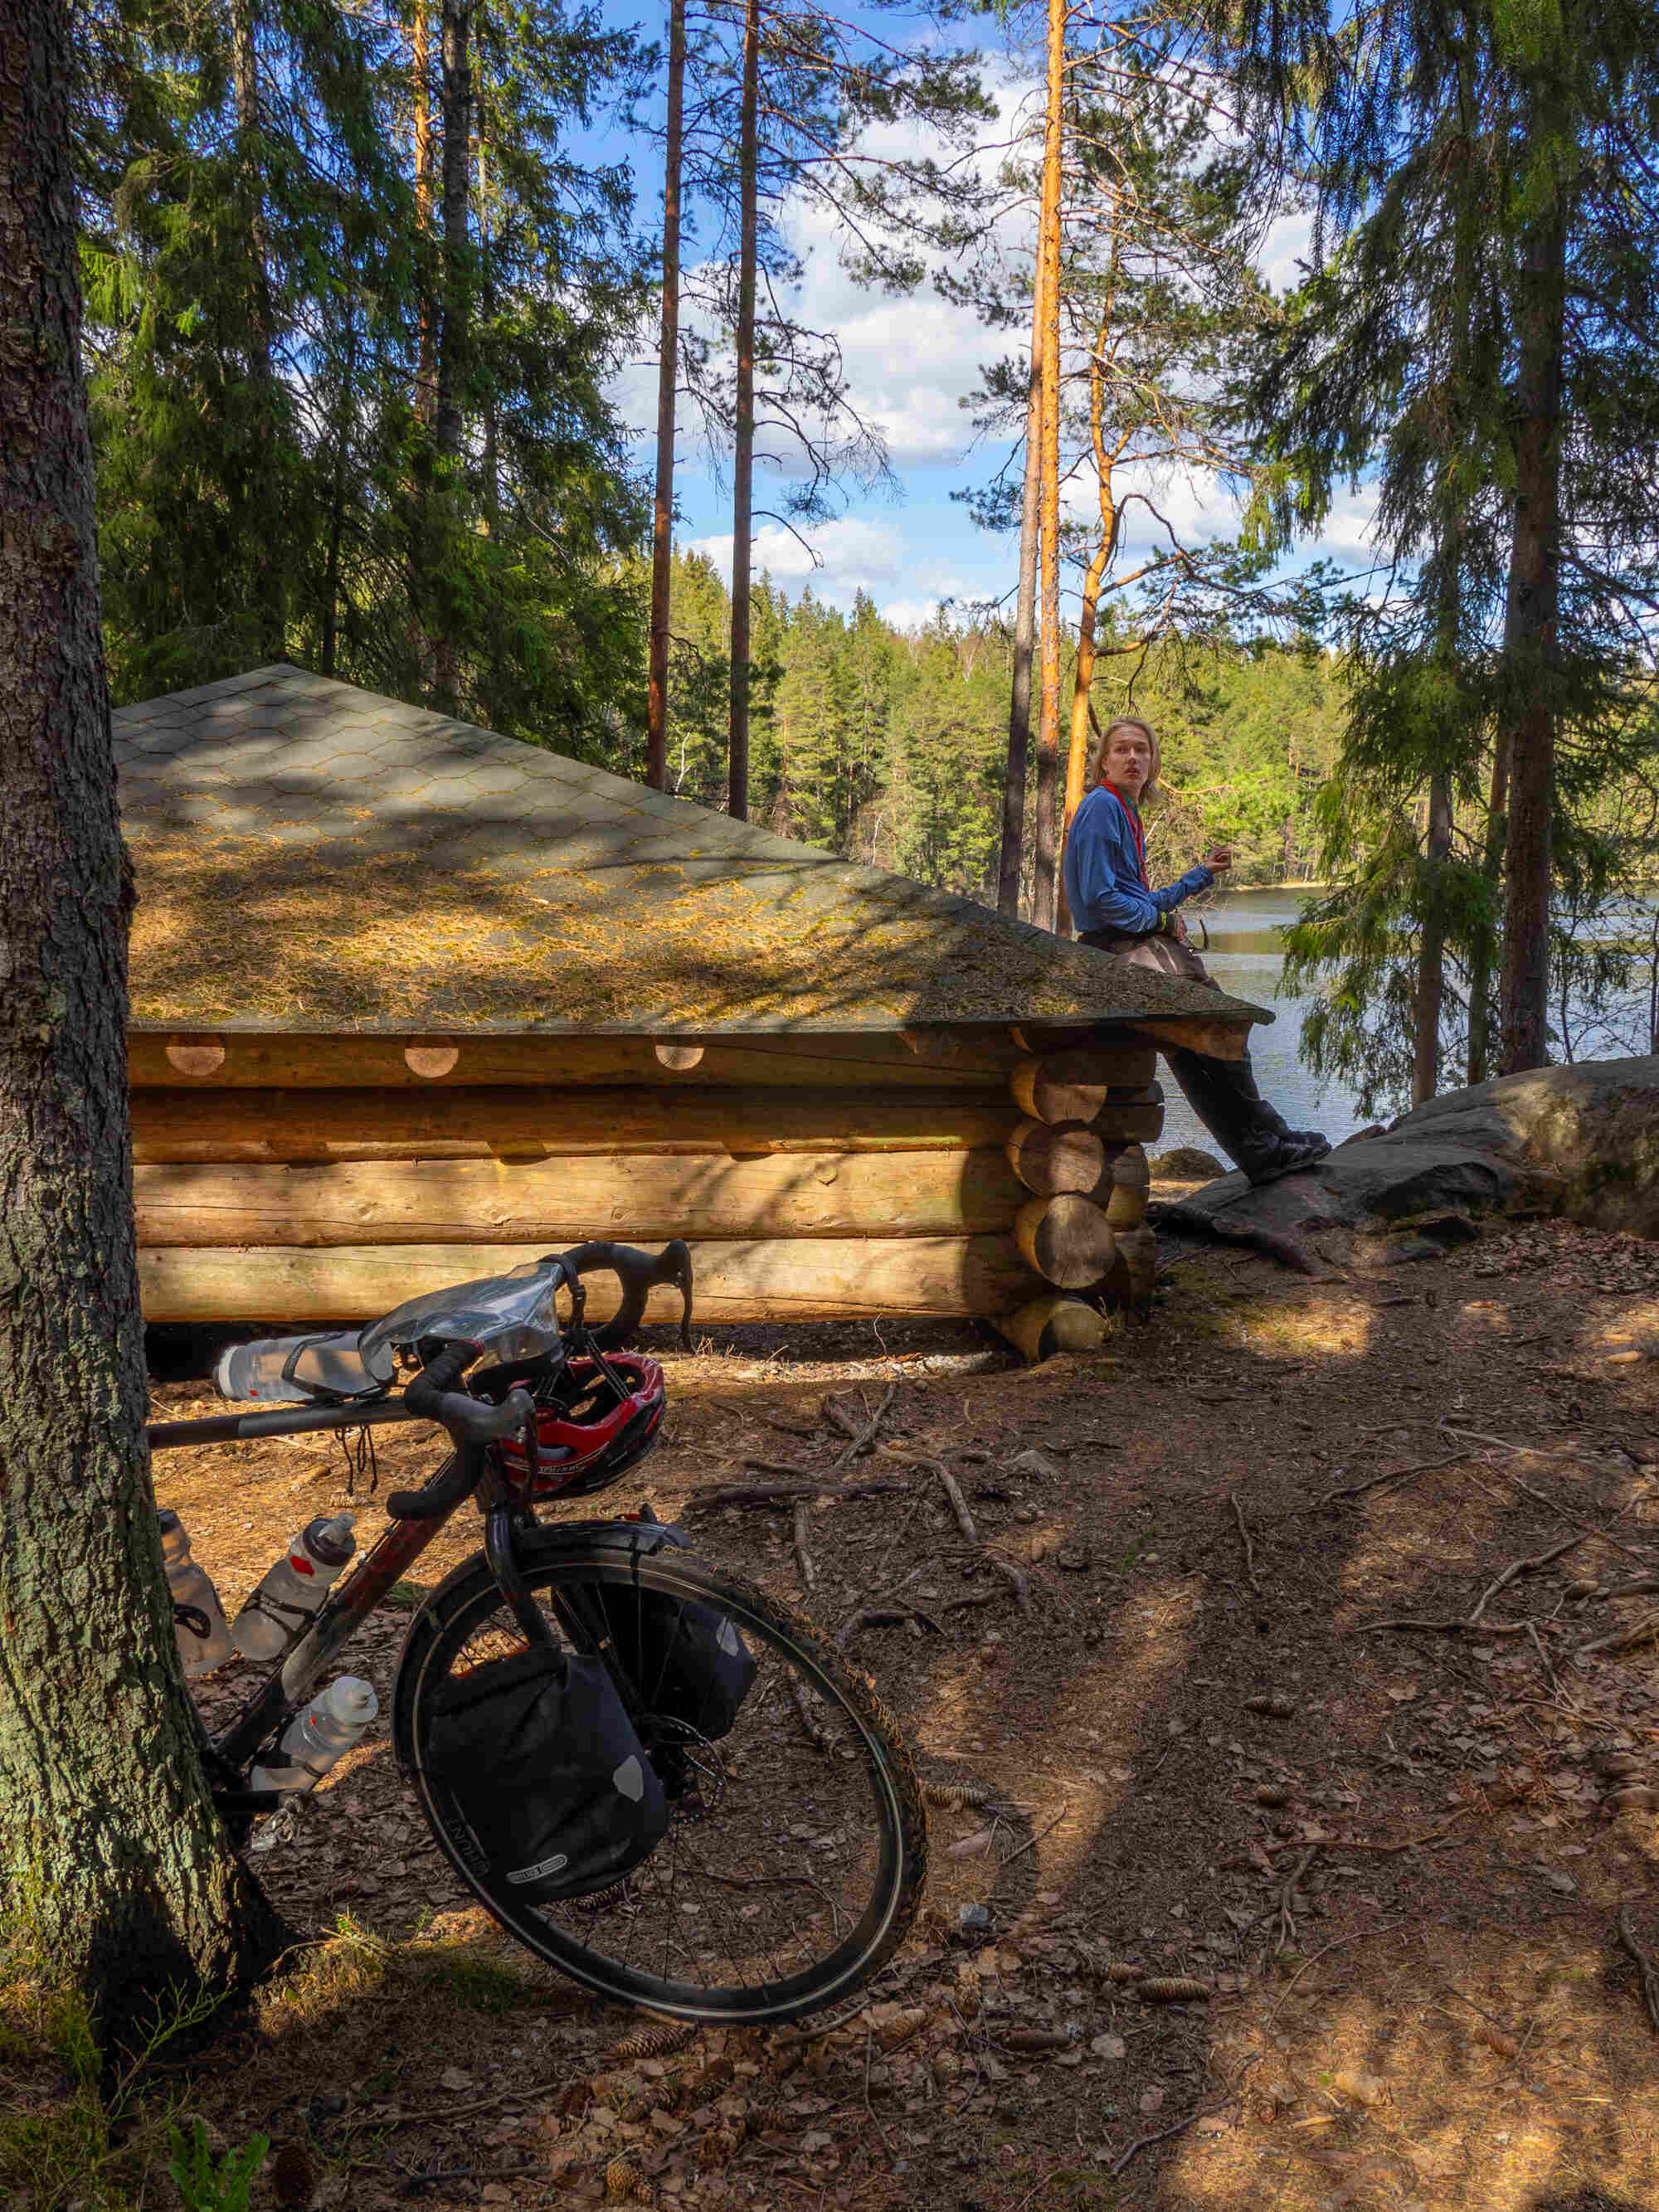
\includegraphics[width=1.05\linewidth]{assets/pyörävaellus11}
			\noindent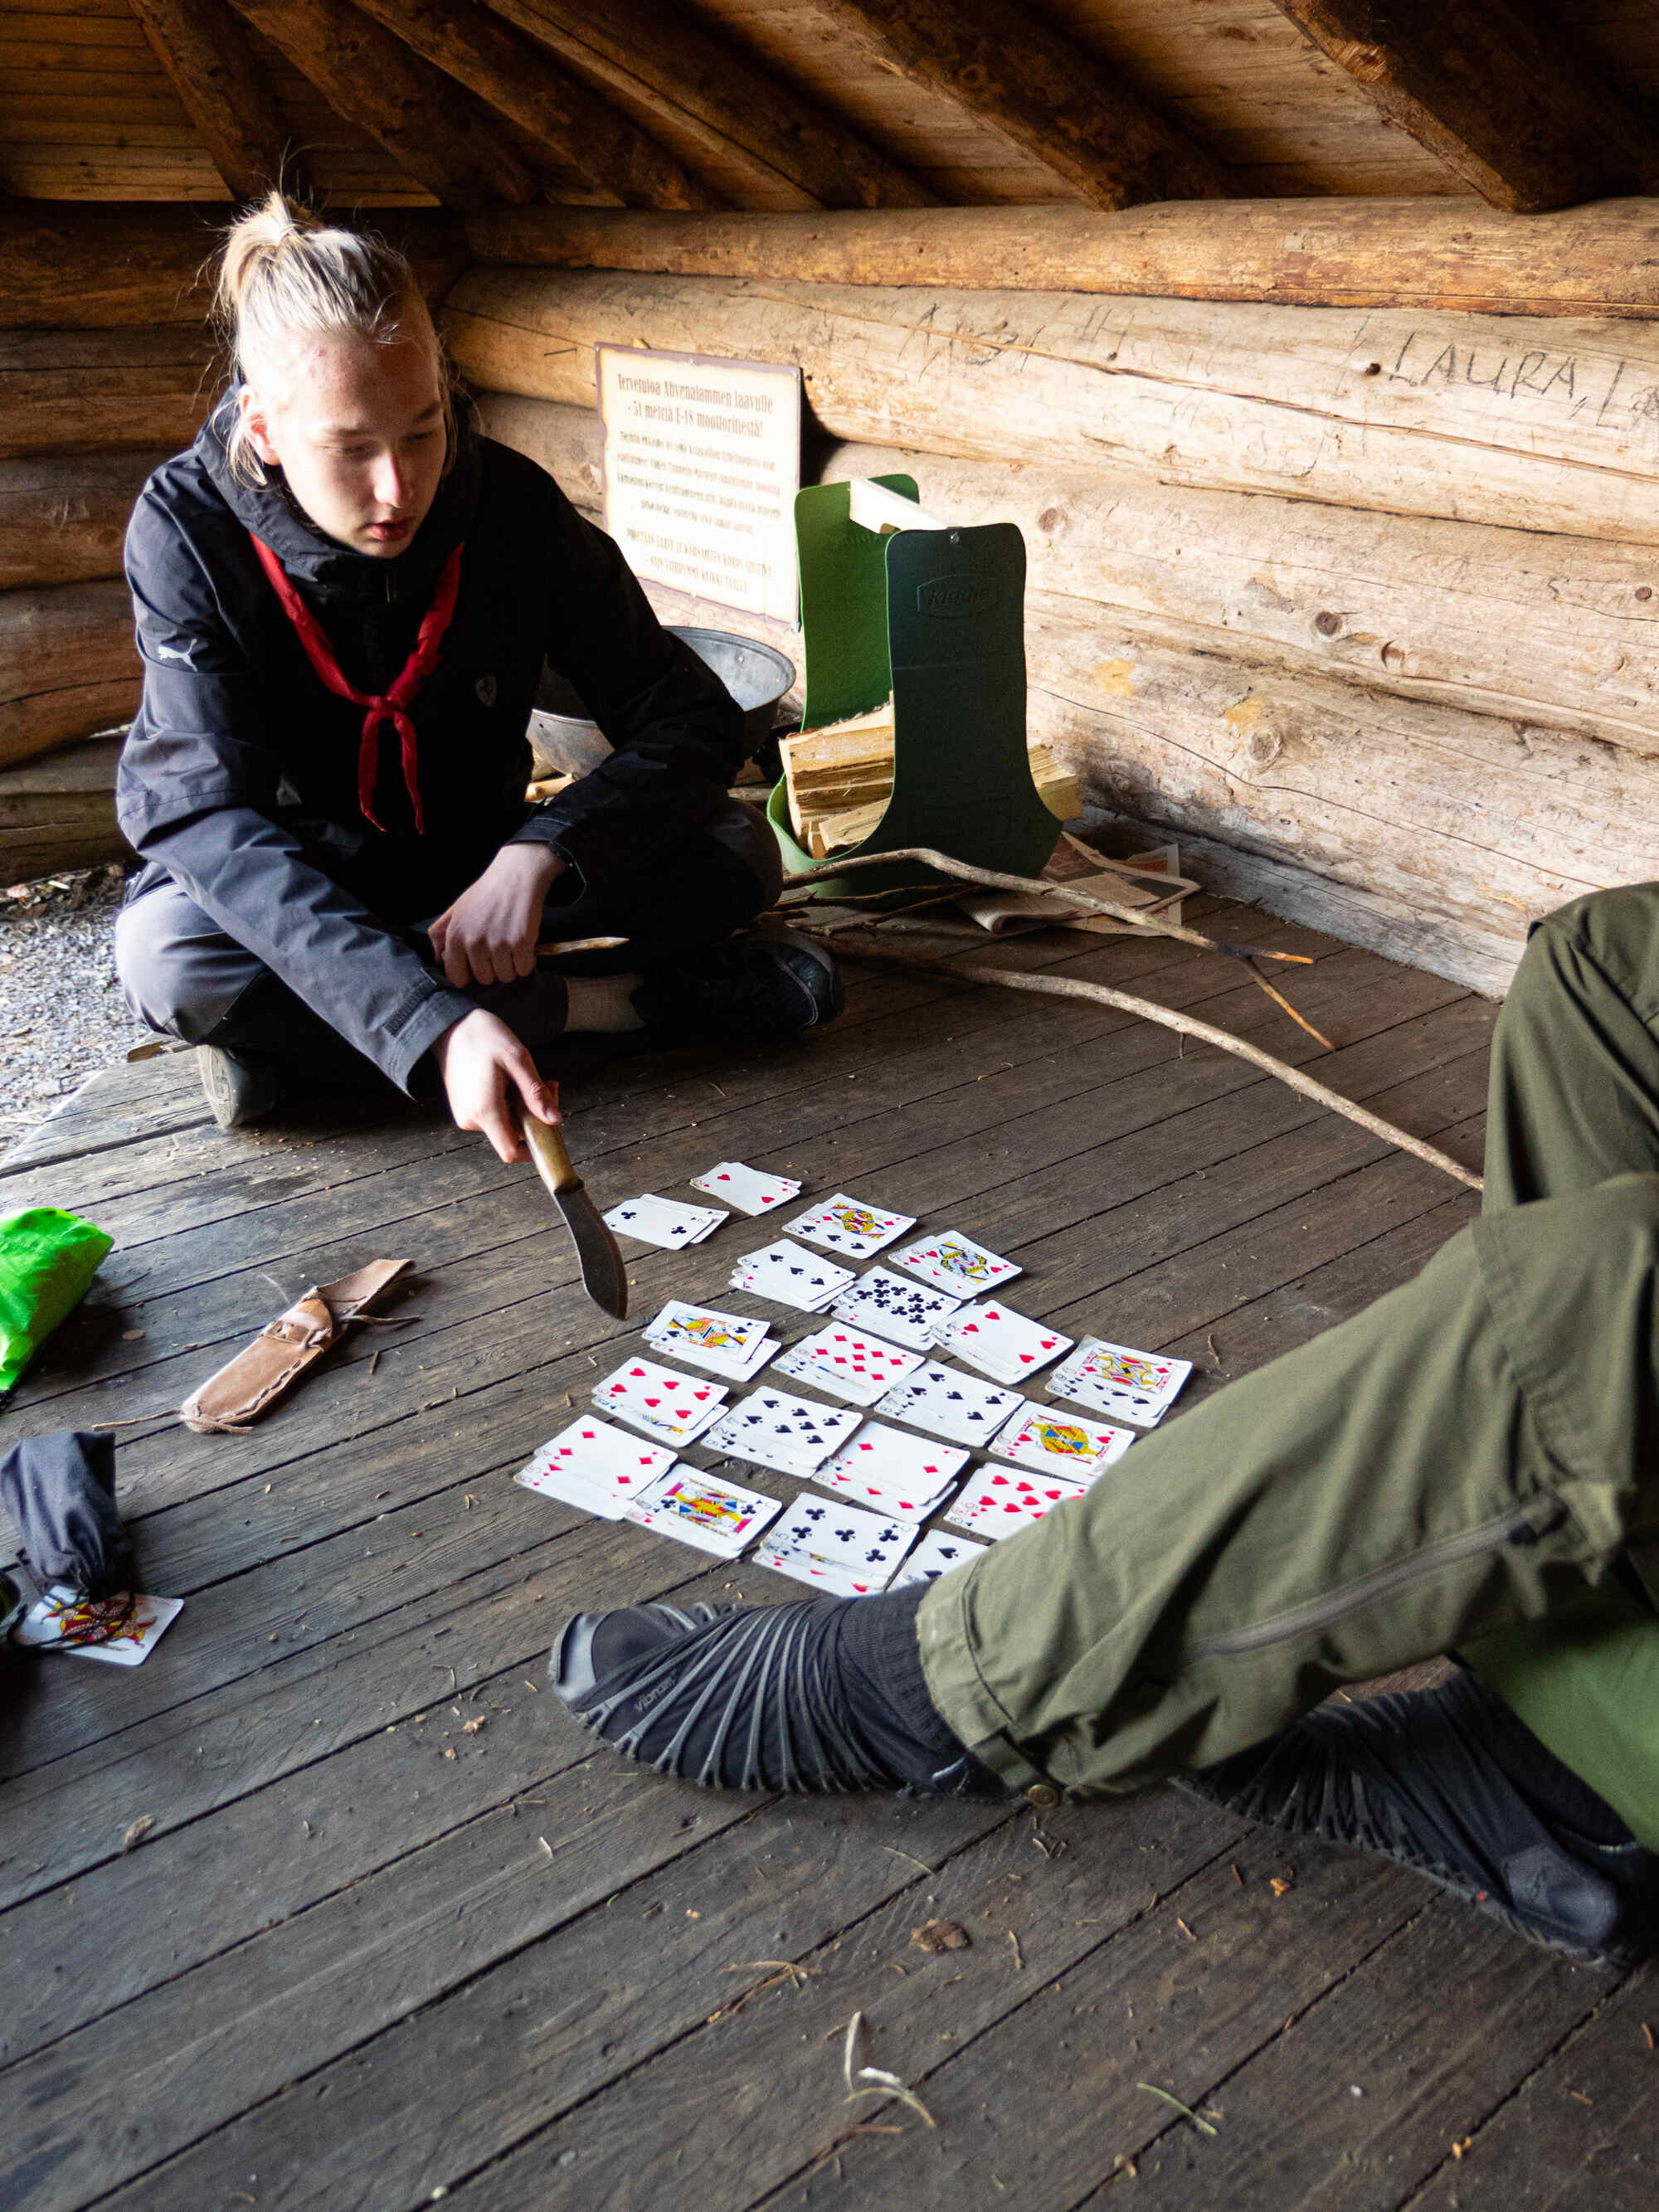
\includegraphics[width=1.05\linewidth]{assets/pyörävaellus15}
		\end{center}
	\end{multicols}
	\vspace*{-0.32cm}
	\captionof{figure}{Ja 47~km jälkeen löytyi meidän seuraava
	yöpymispaikkamme: Ahvenalampi, Lohja.}
\end{center}
\end{Figure}


\begin{Figure}
	\noindent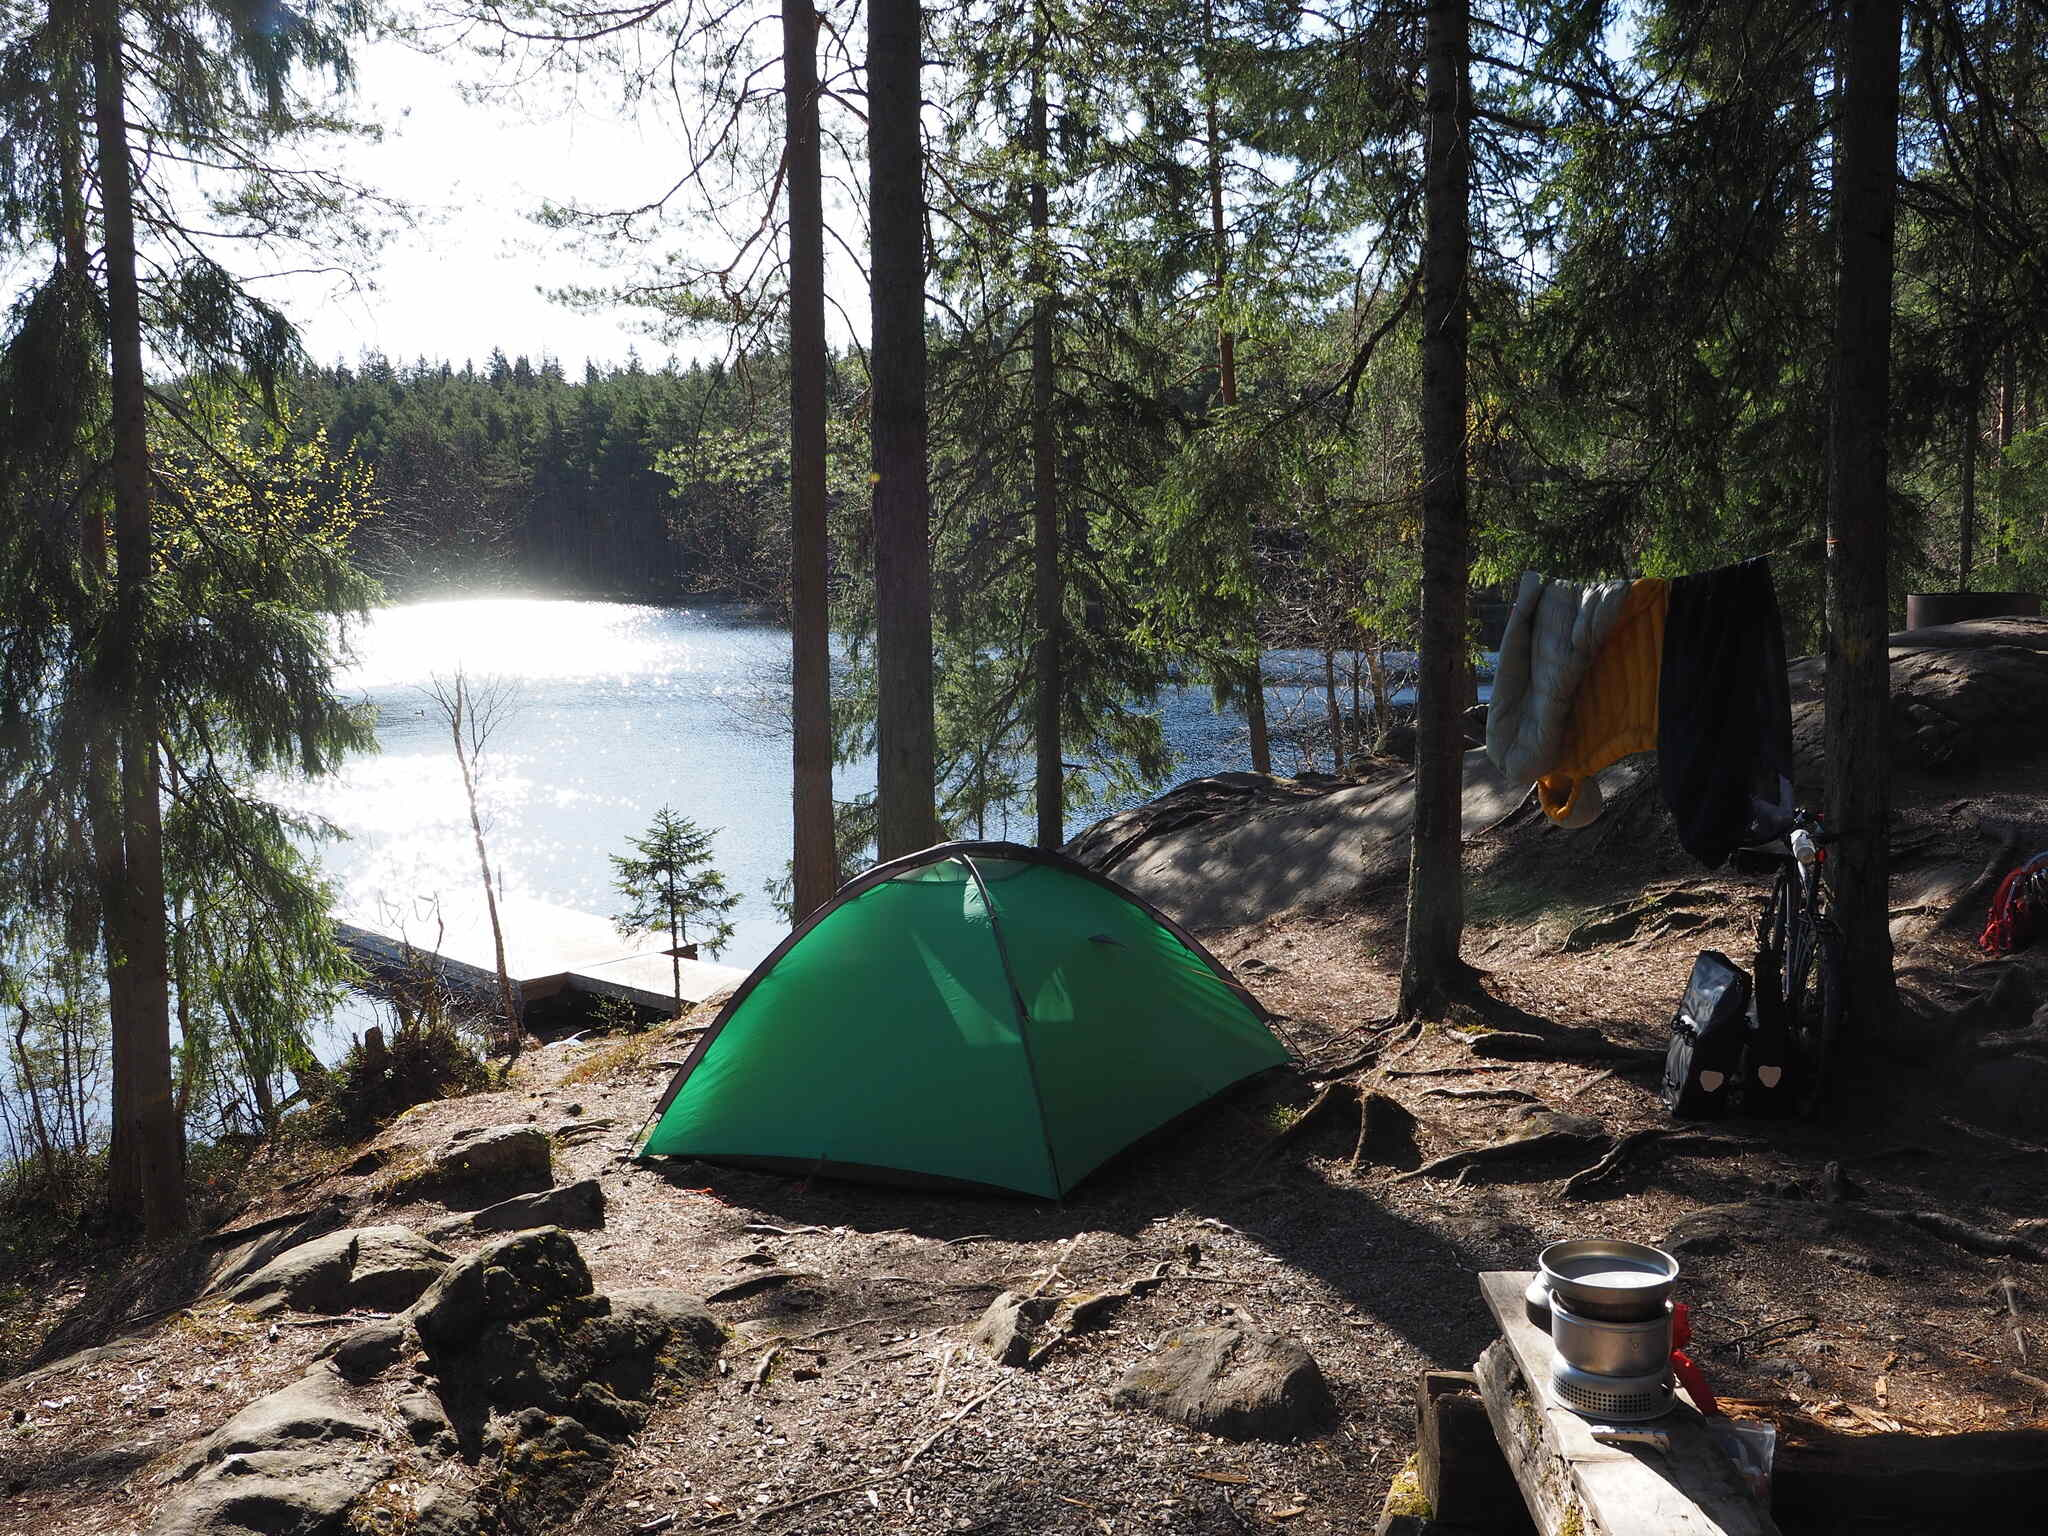
\includegraphics[width=\linewidth]{assets/pyörävaellus16}
	\captionof{figure}{Hauska fakta: Nukuimme suoraan
	Helsinki"-Turku"-moottoritien päällä, joka kulki yöpymispaikan alla tunnelin läpi.}
\end{Figure}

\begin{multicols}{2}
	\begin{center}
		\noindent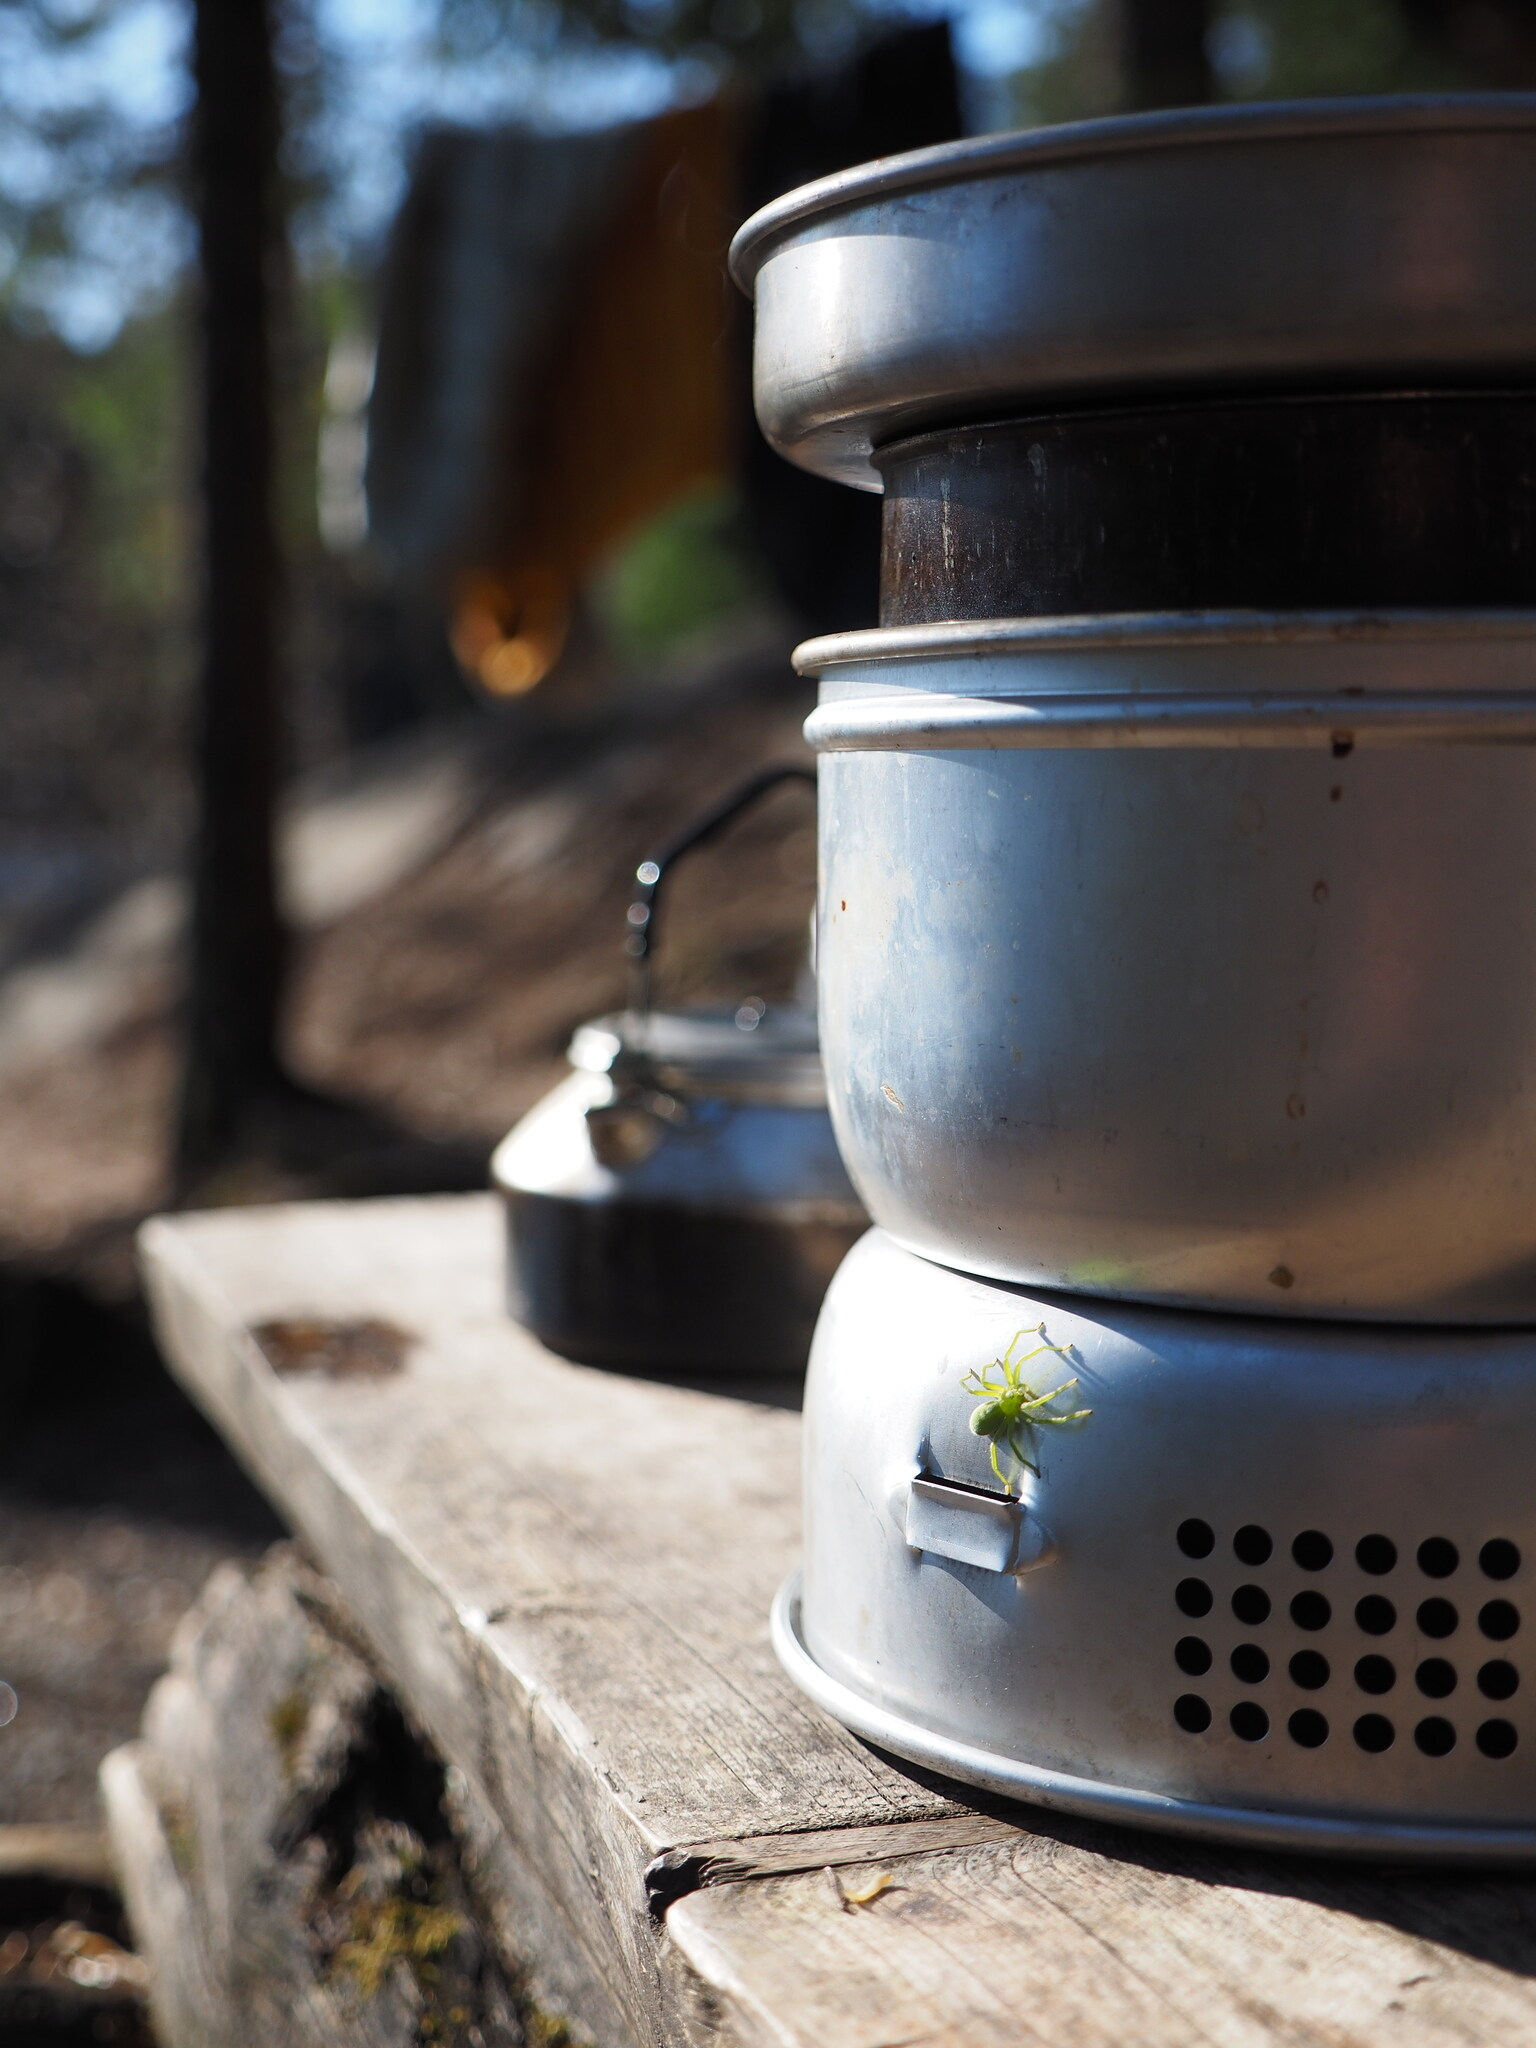
\includegraphics[height=0.36\paperheight]{assets/pyörävaellus17}
	\end{center}
	\columnbreak
	\begin{Figure}
		\noindent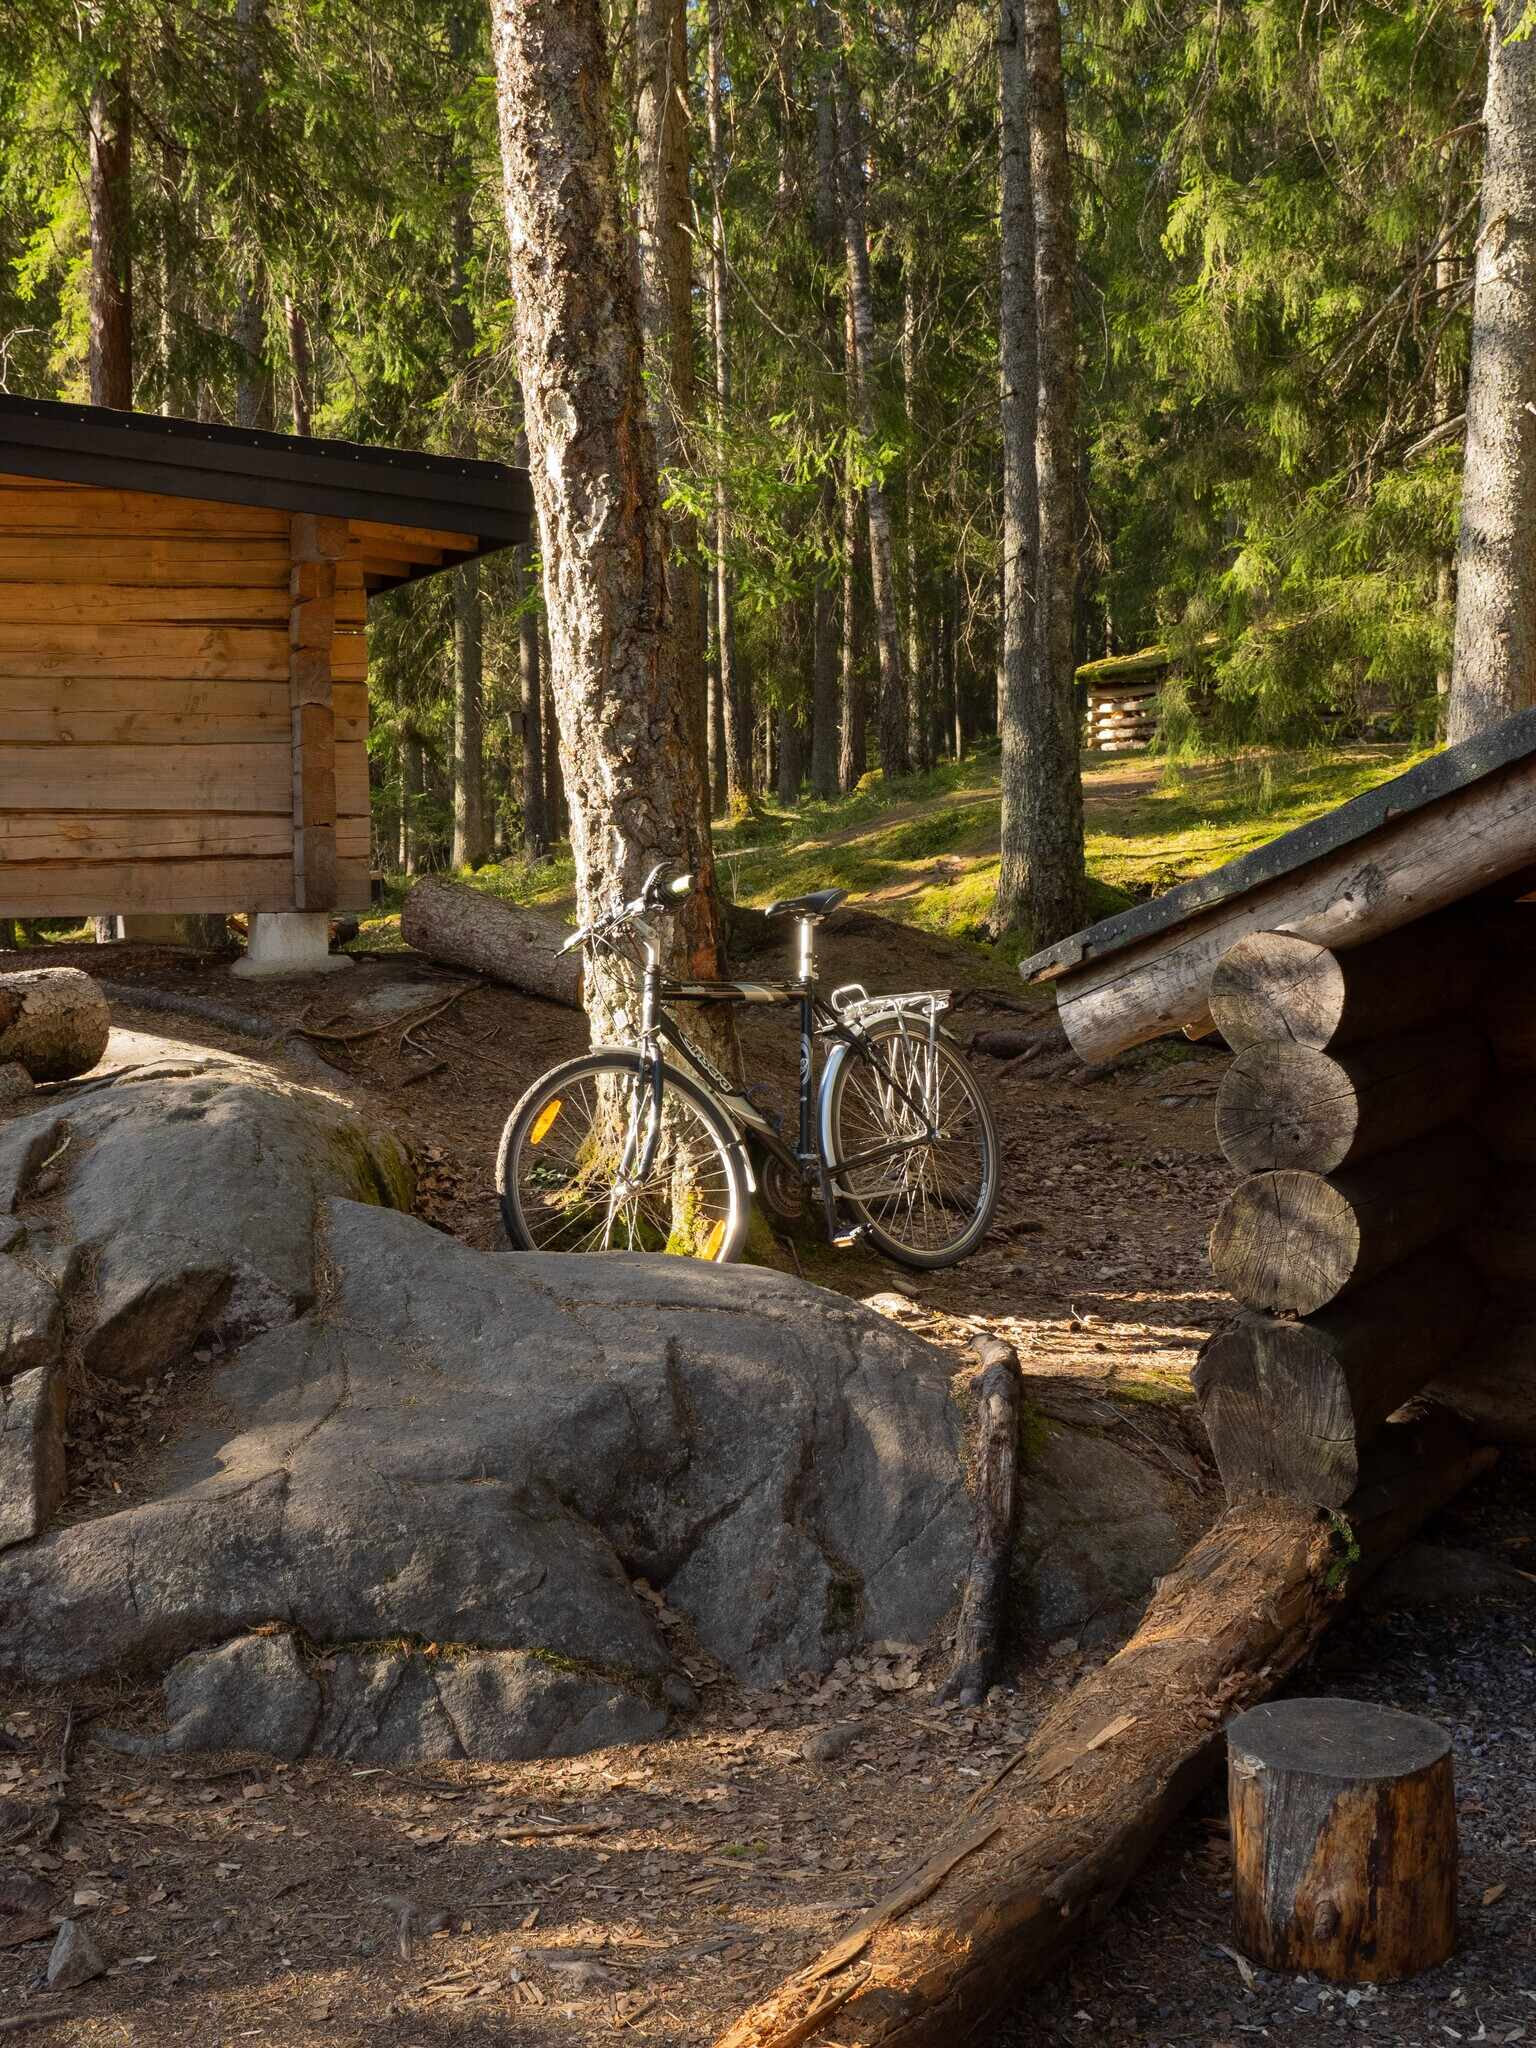
\includegraphics[height=0.36\paperheight]{assets/pyörävaellus18}
	\end{Figure}
\end{multicols}


\begin{Figure}
	\noindent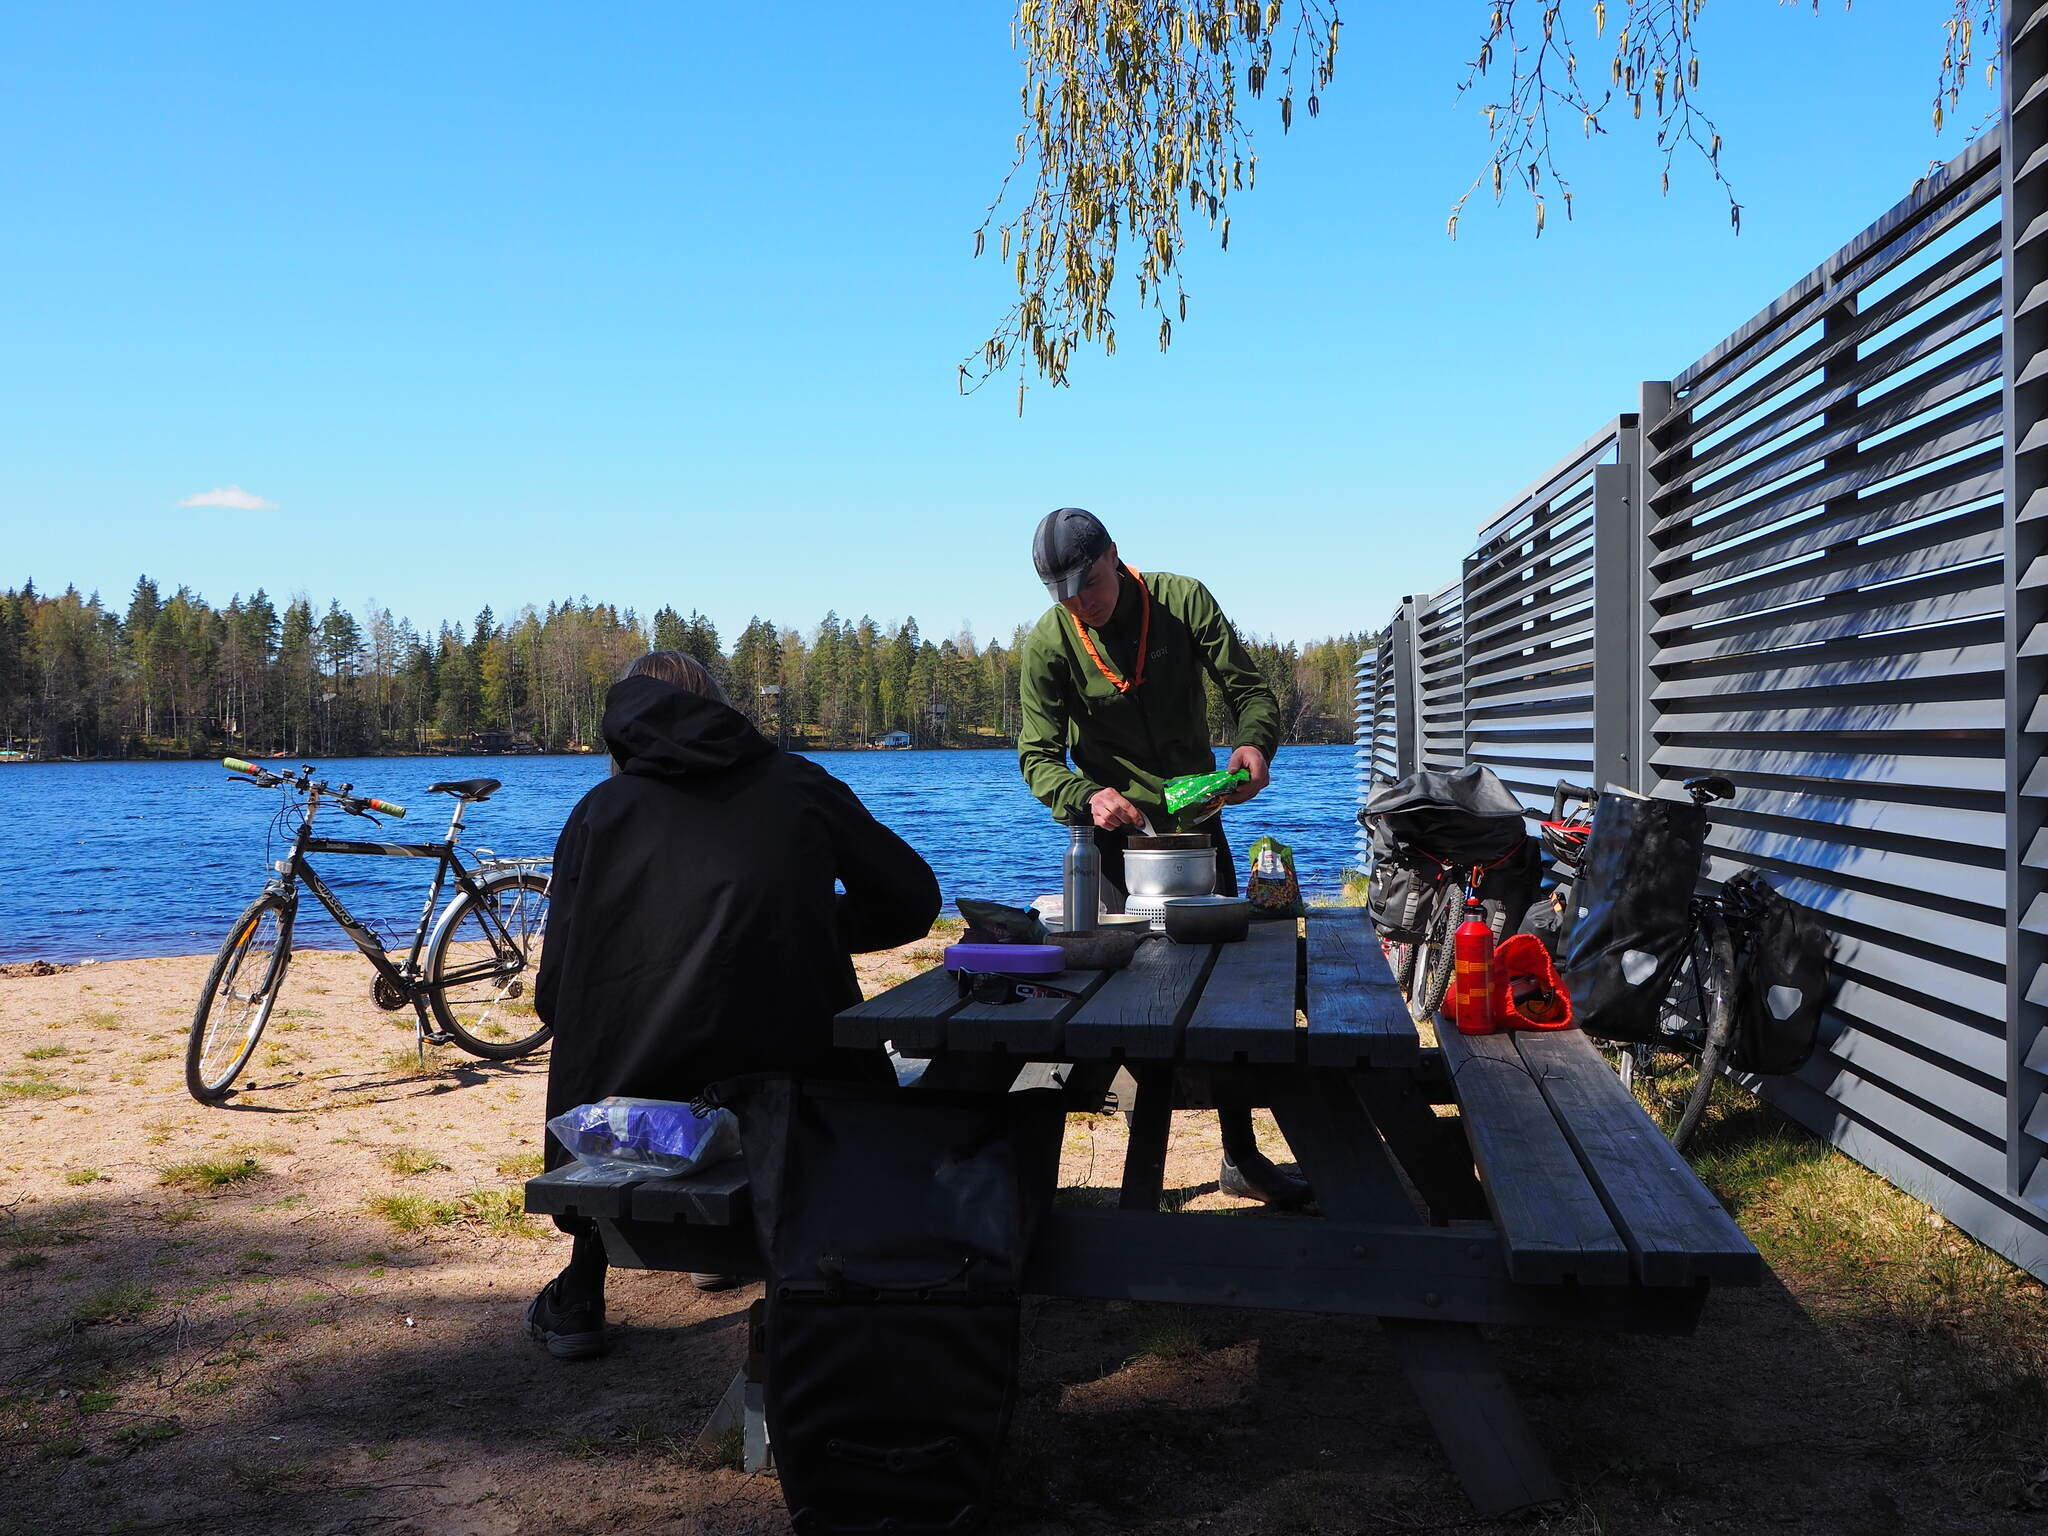
\includegraphics[width=\linewidth]{assets/pyörävaellus19}
	\captionof{figure}{Kolmas päivä oli taas aika pitkä ja vei meidät itään, ensiksi Vihtiin. Lounastauko otettiin Nummelan Myllylammen uimarannalla ja jatketiin matkaa kohti Espoon Vääräjärveä.}
\end{Figure}

\begin{multicols}{2}
	\begin{center}
		\noindent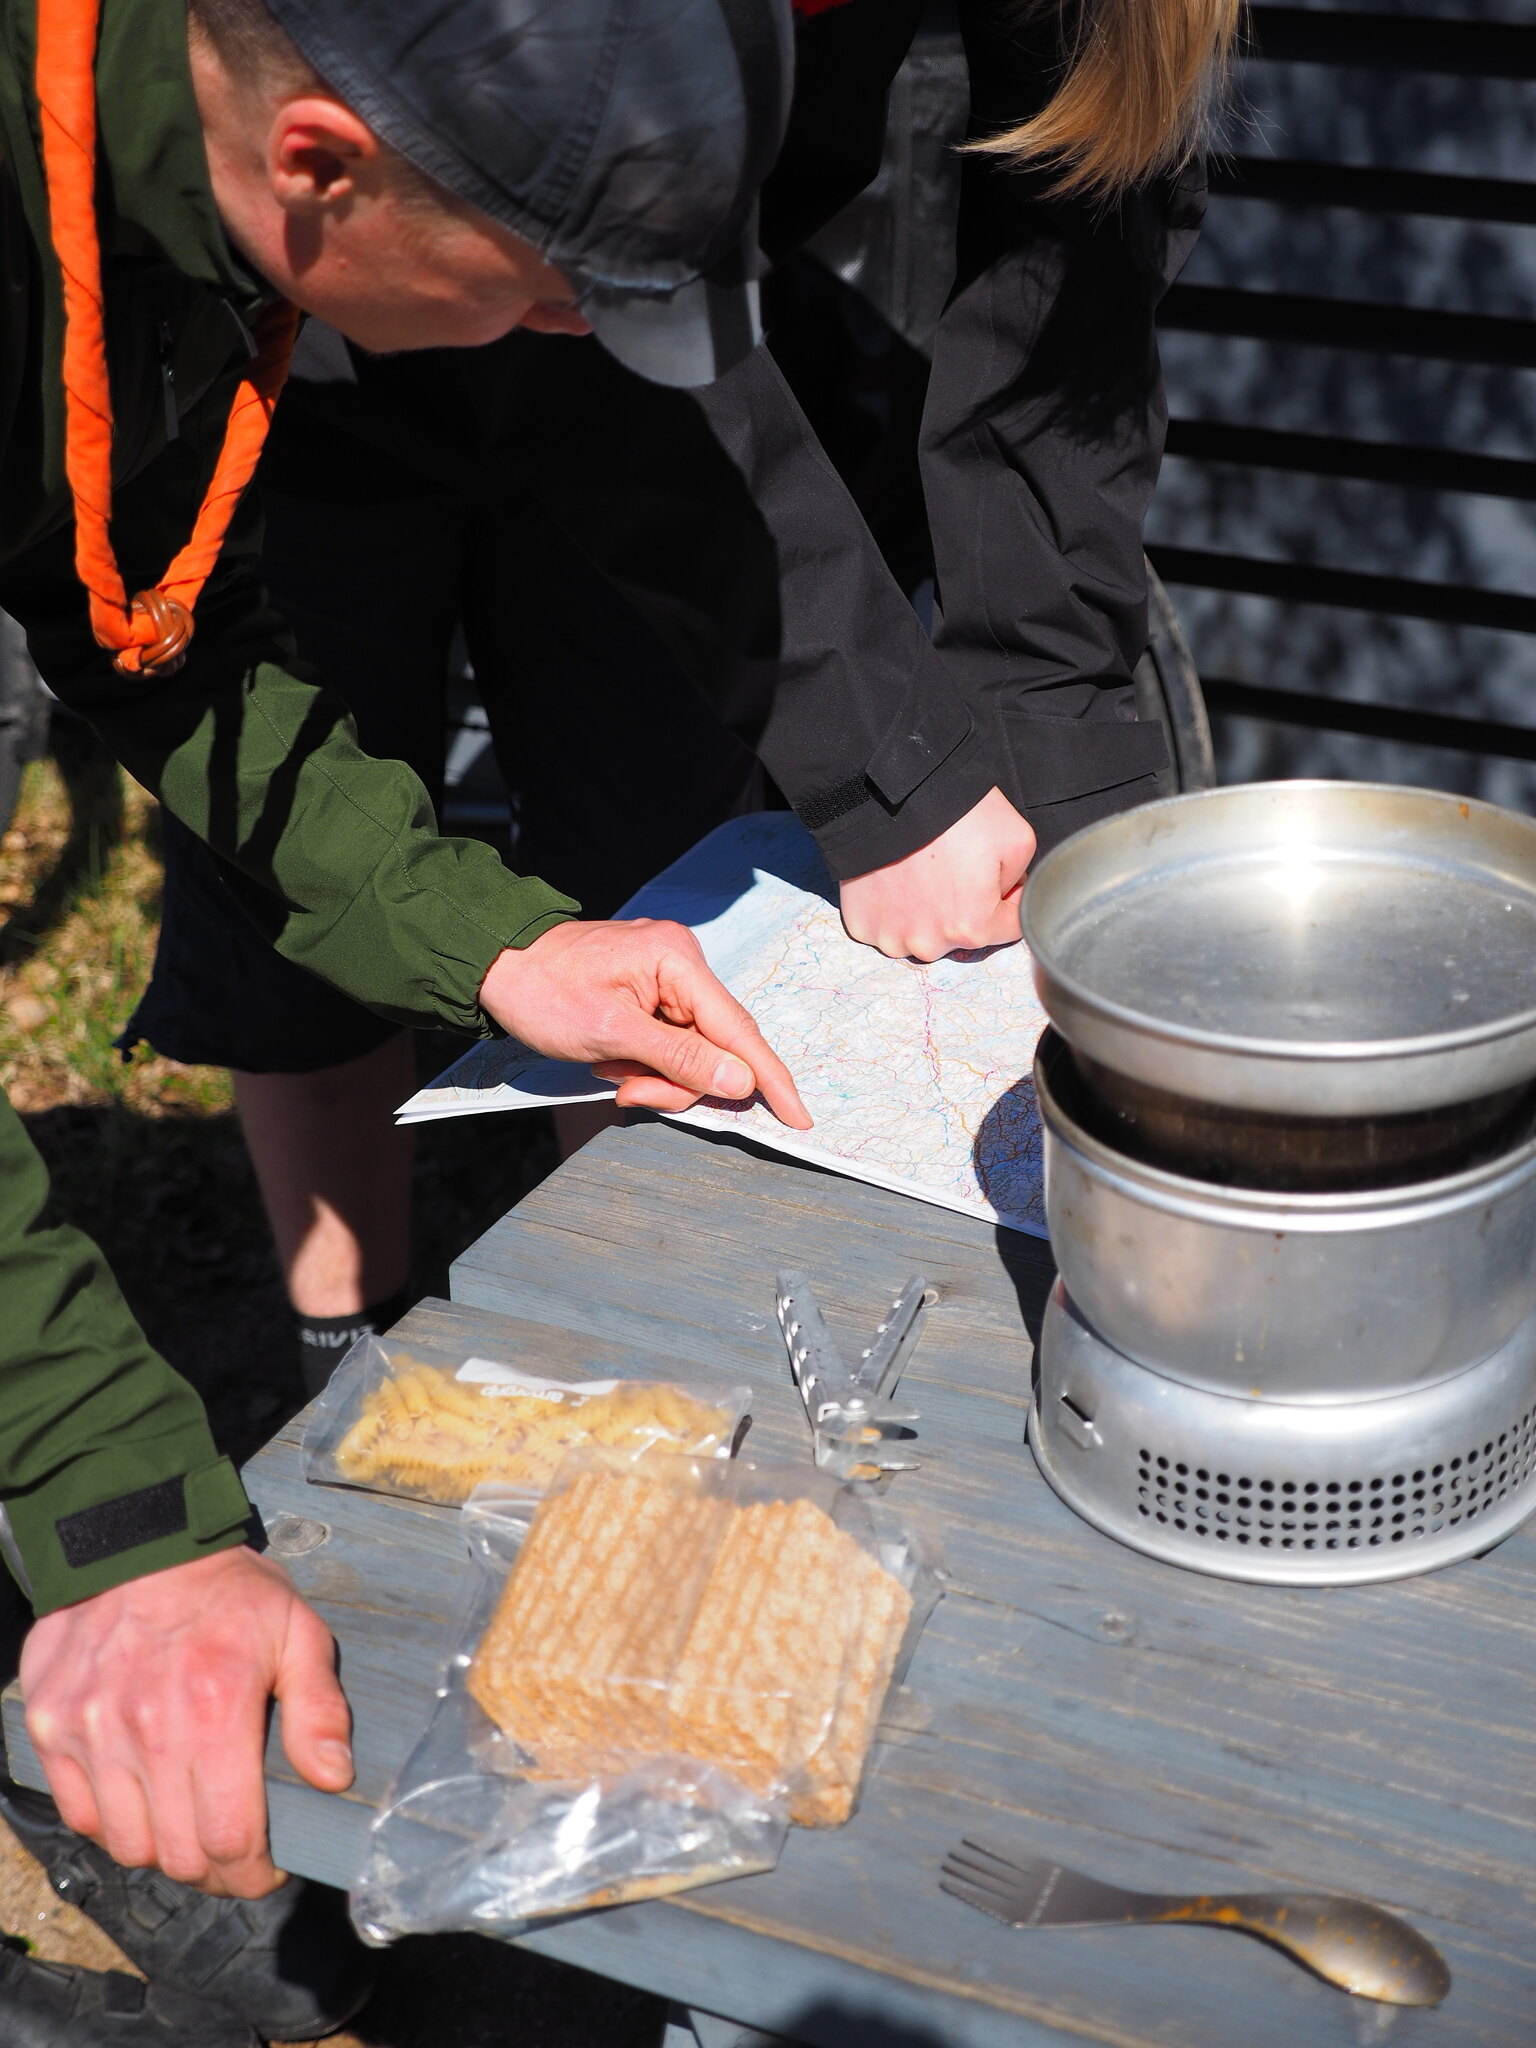
\includegraphics[height=0.36\paperheight]{assets/pyörävaellus20}
	\end{center}
	\columnbreak
	\begin{Figure}
		\noindent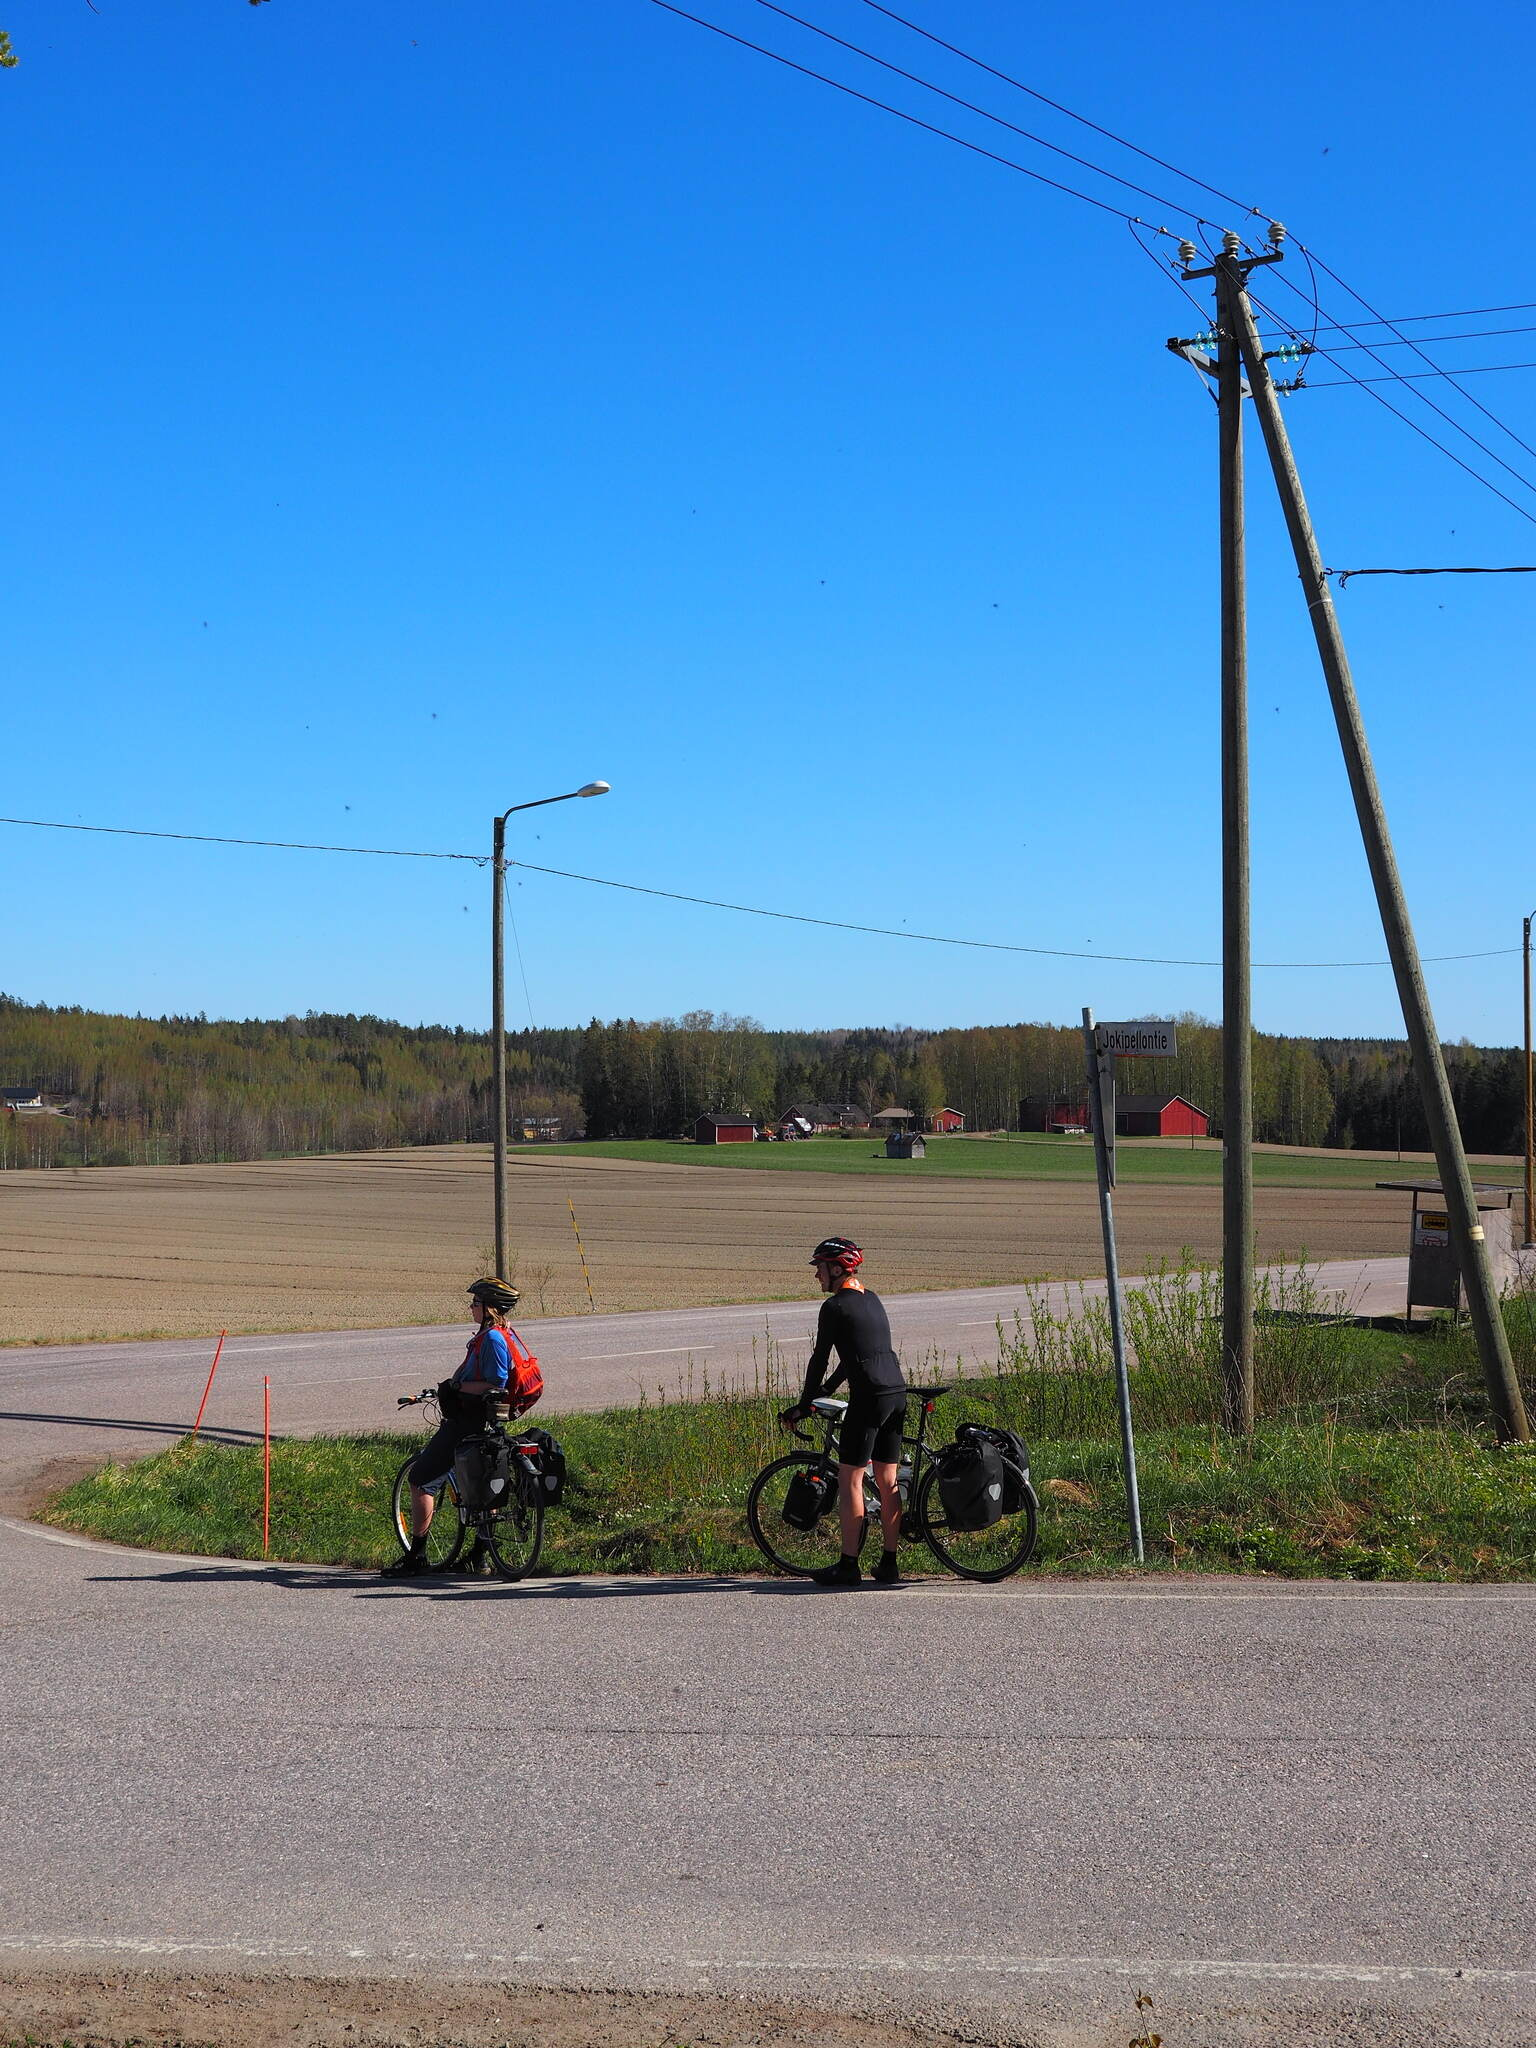
\includegraphics[height=0.36\paperheight]{assets/pyörävaellus21}
	\end{Figure}
\end{multicols}


\begin{multicols}{2}
	\begin{center}
		\noindent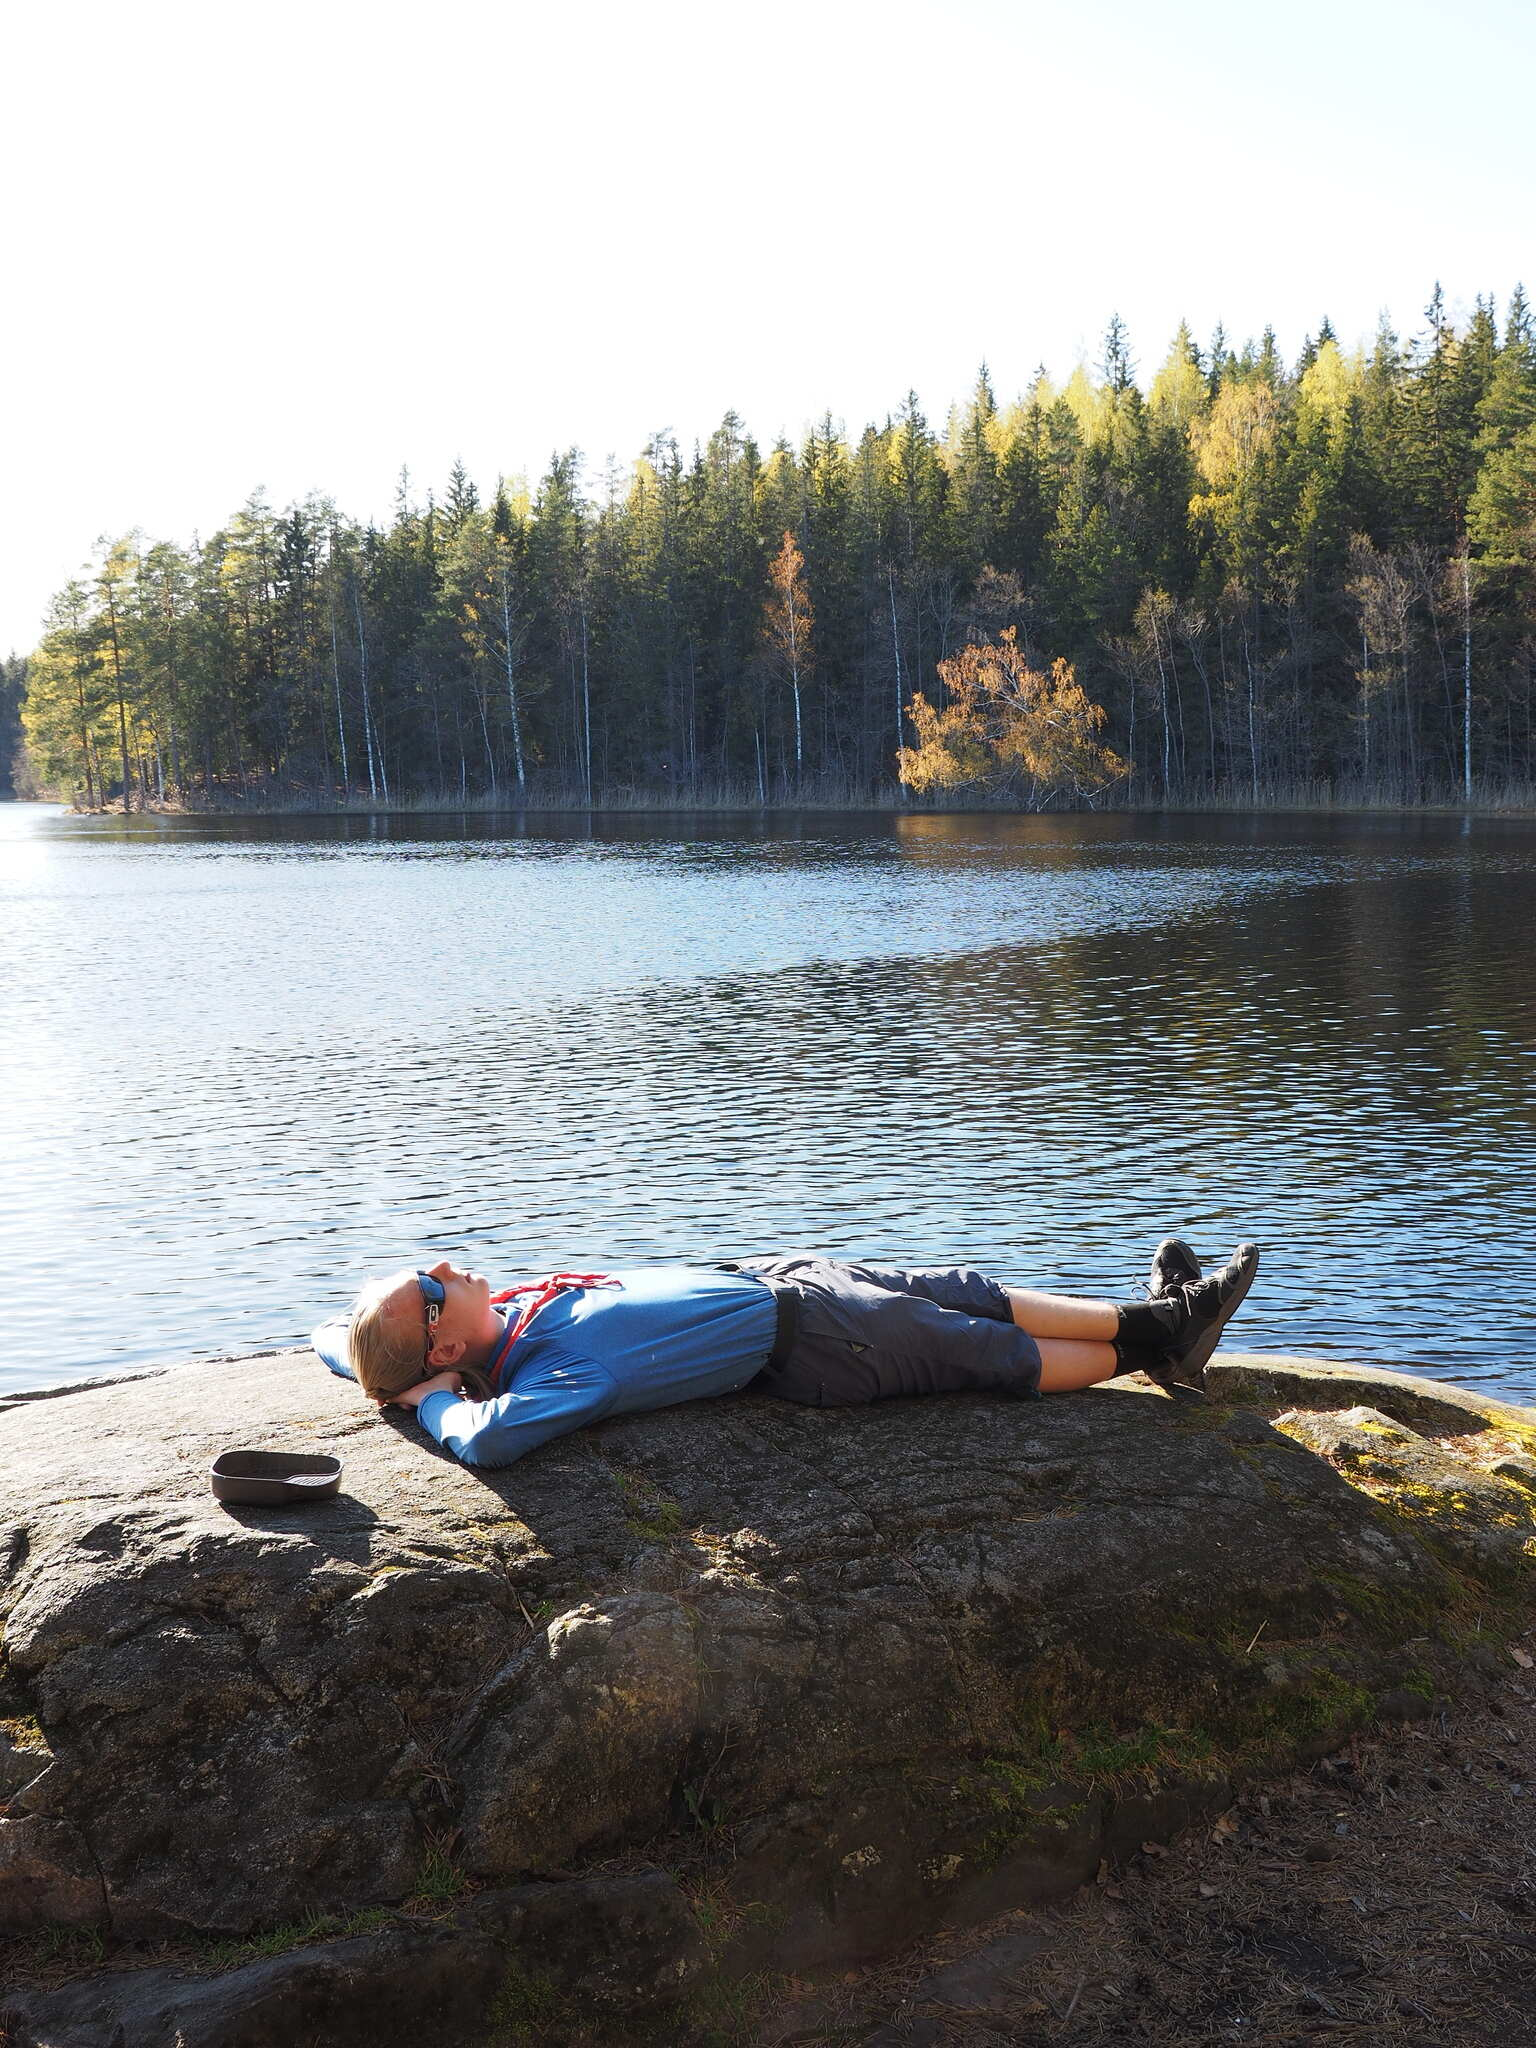
\includegraphics[width=1.05\linewidth]{assets/pyörävaellus24}
		\noindent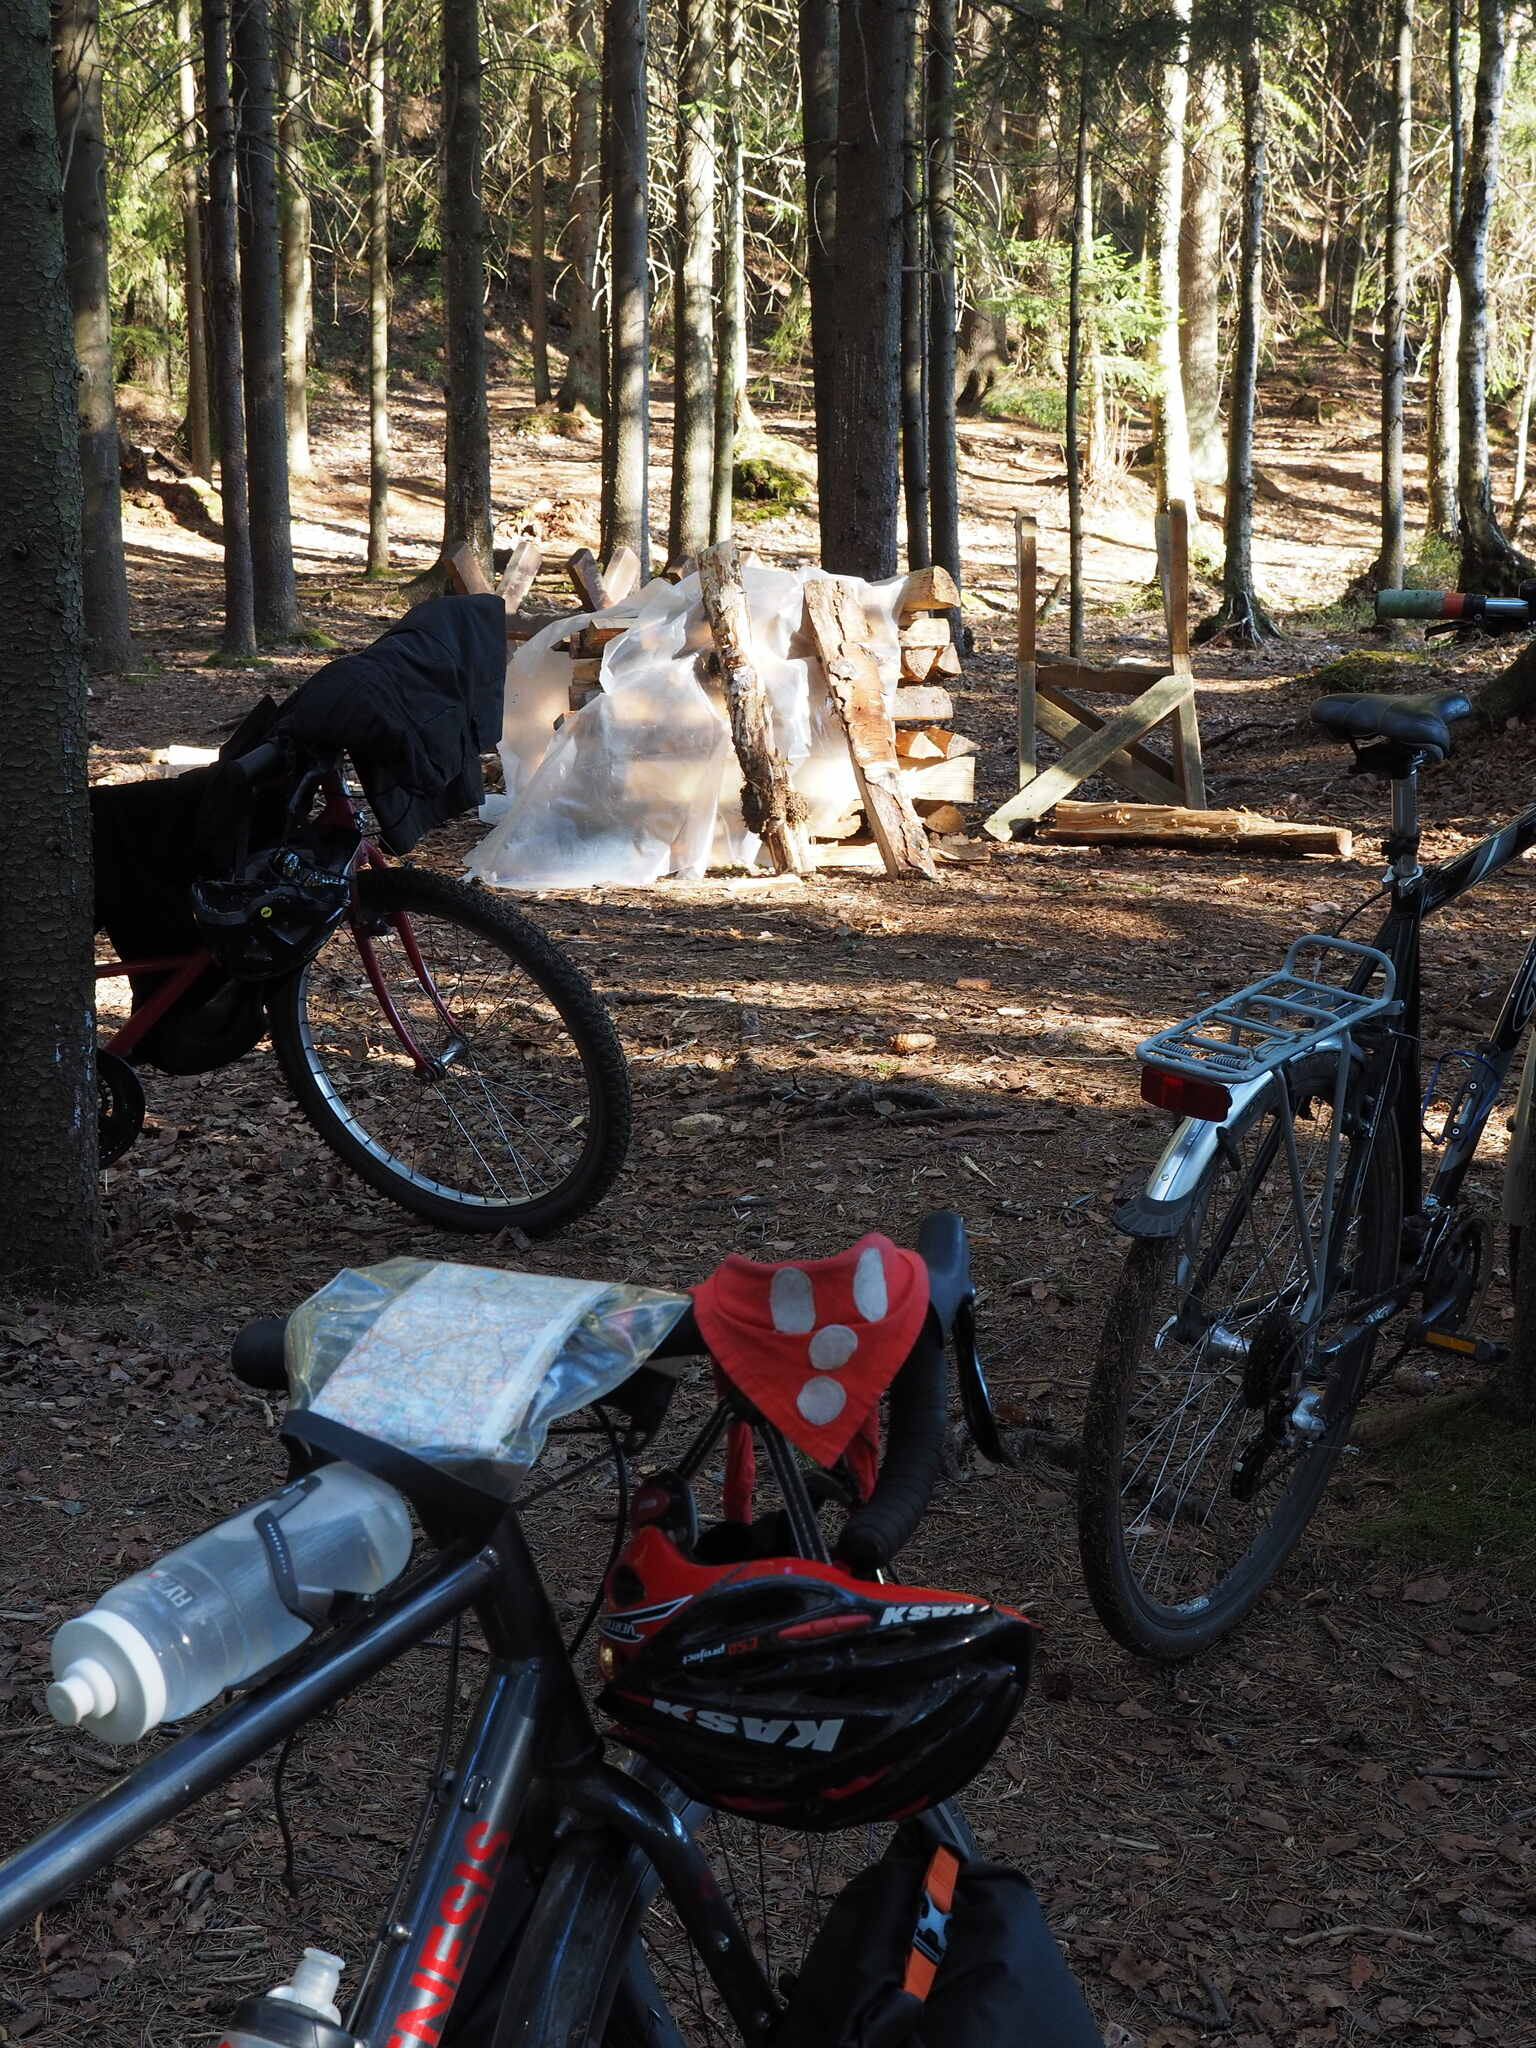
\includegraphics[width=1.05\linewidth]{assets/pyörävaellus22}
	\end{center}
	\columnbreak
	\begin{center}
		\noindent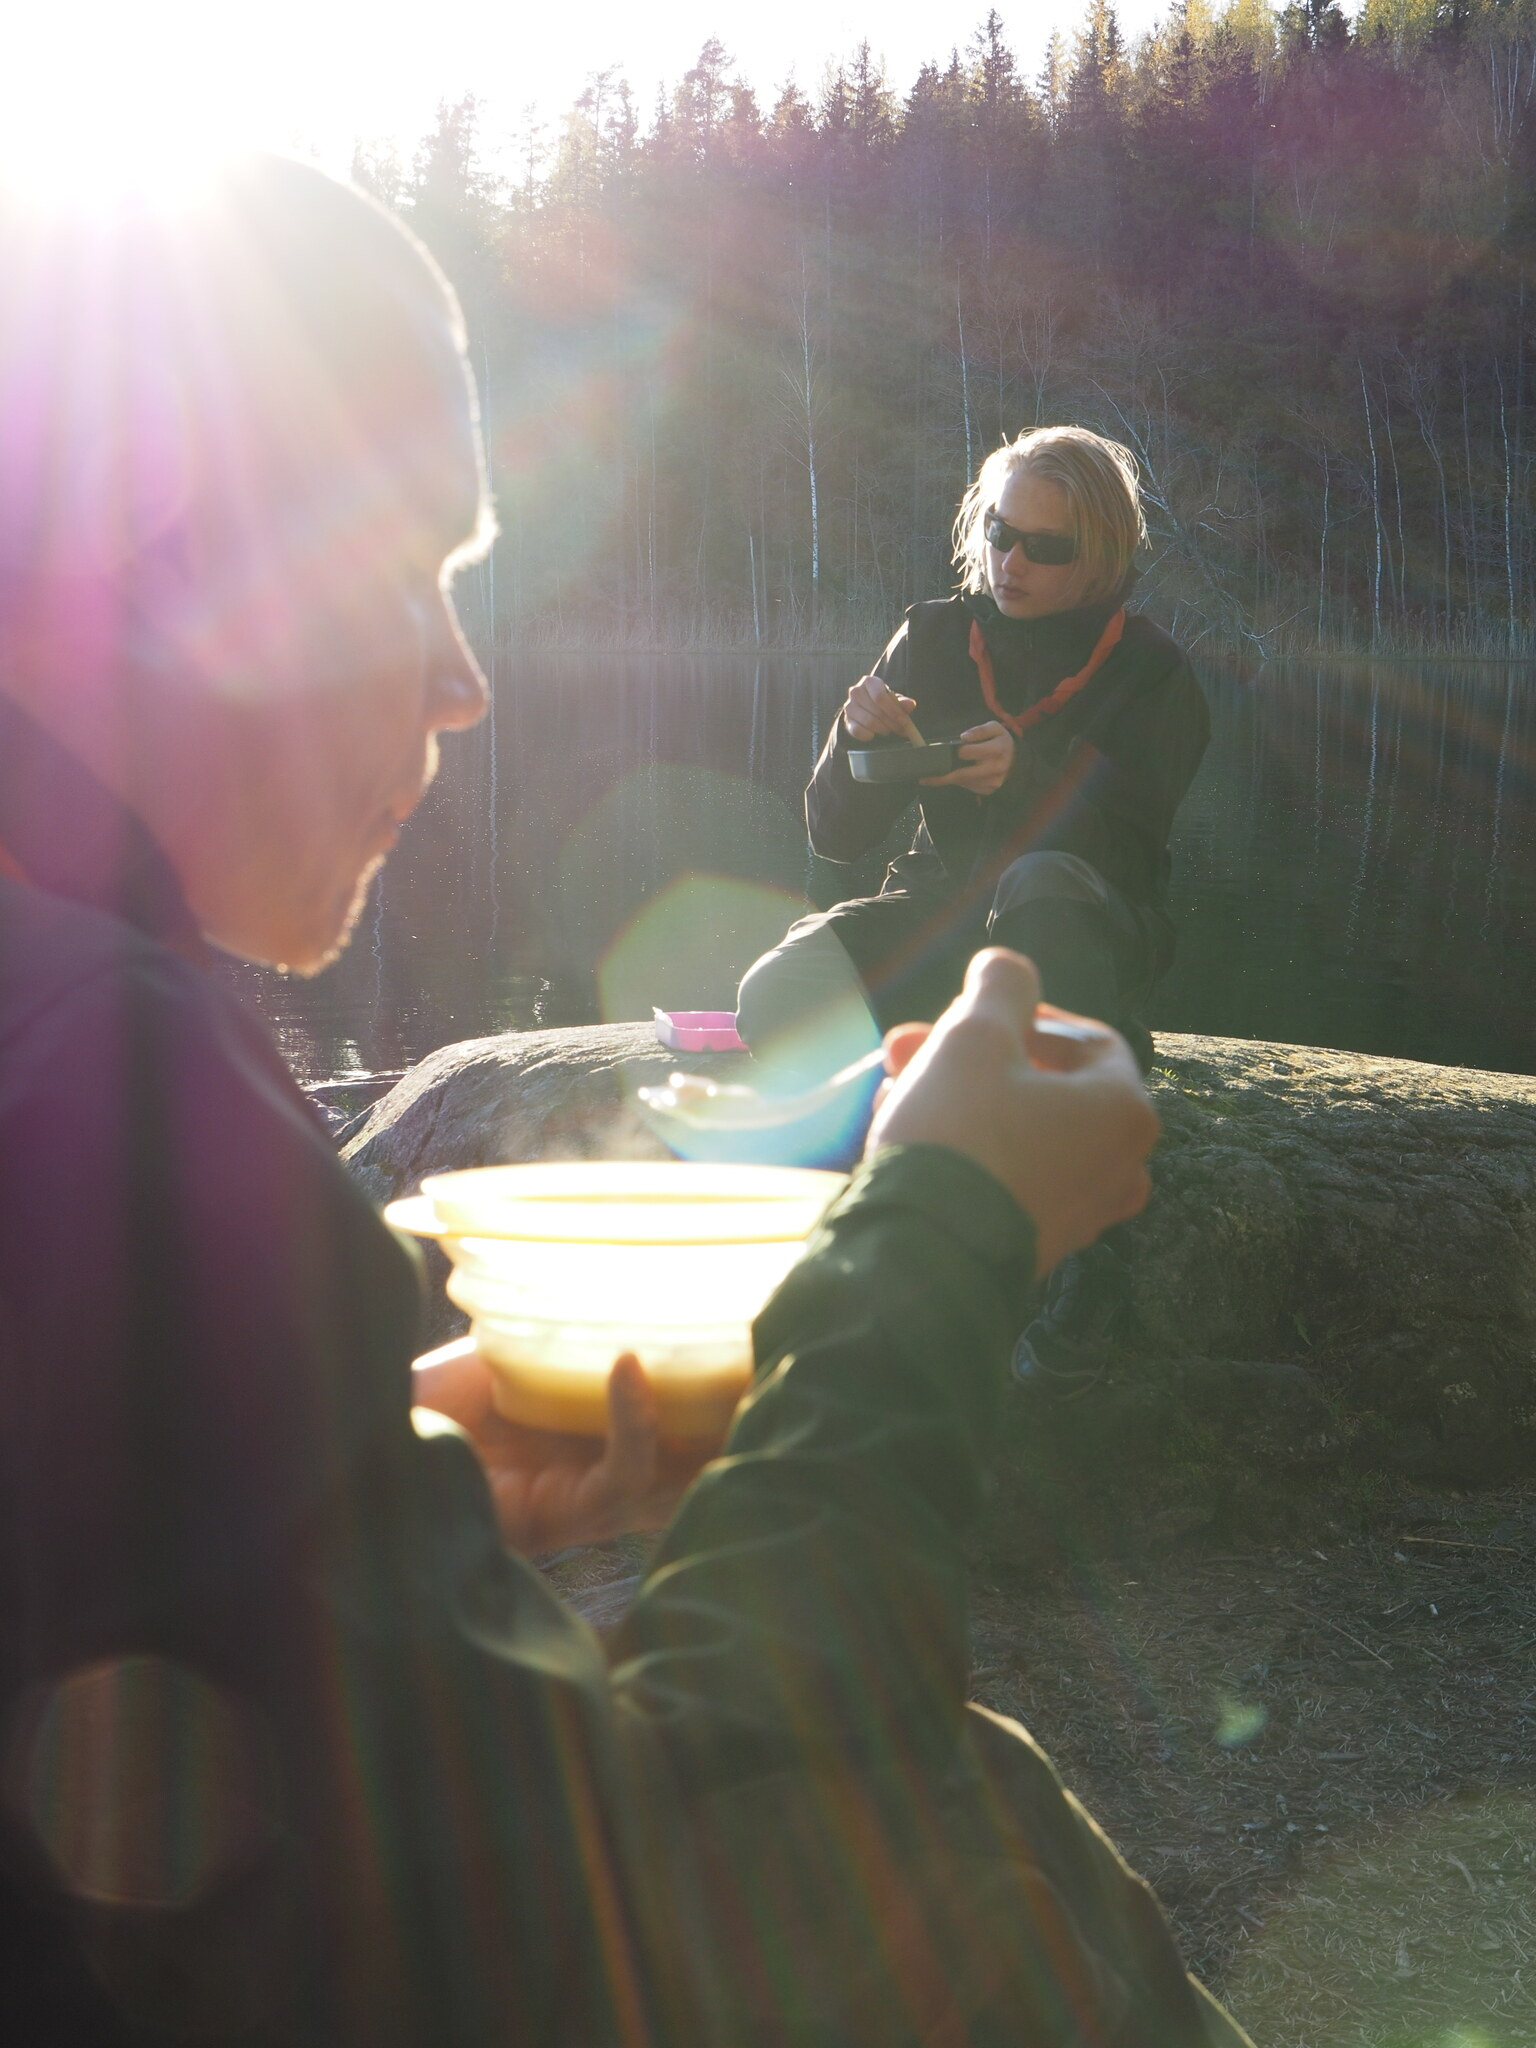
\includegraphics[width=1.05\linewidth]{assets/pyörävaellus23}
	\end{center}
	\begin{addmargin}[0.32cm]{0cm}
		{\small
		64~km päivän jälkeen saavuimme perille meidän viimeiseen
		yöpymispaikkaamme: Vääräjärvi, Espoo.}
	\end{addmargin}
\end{multicols}


\begin{multicols}{2}
	\begin{center}
		\noindent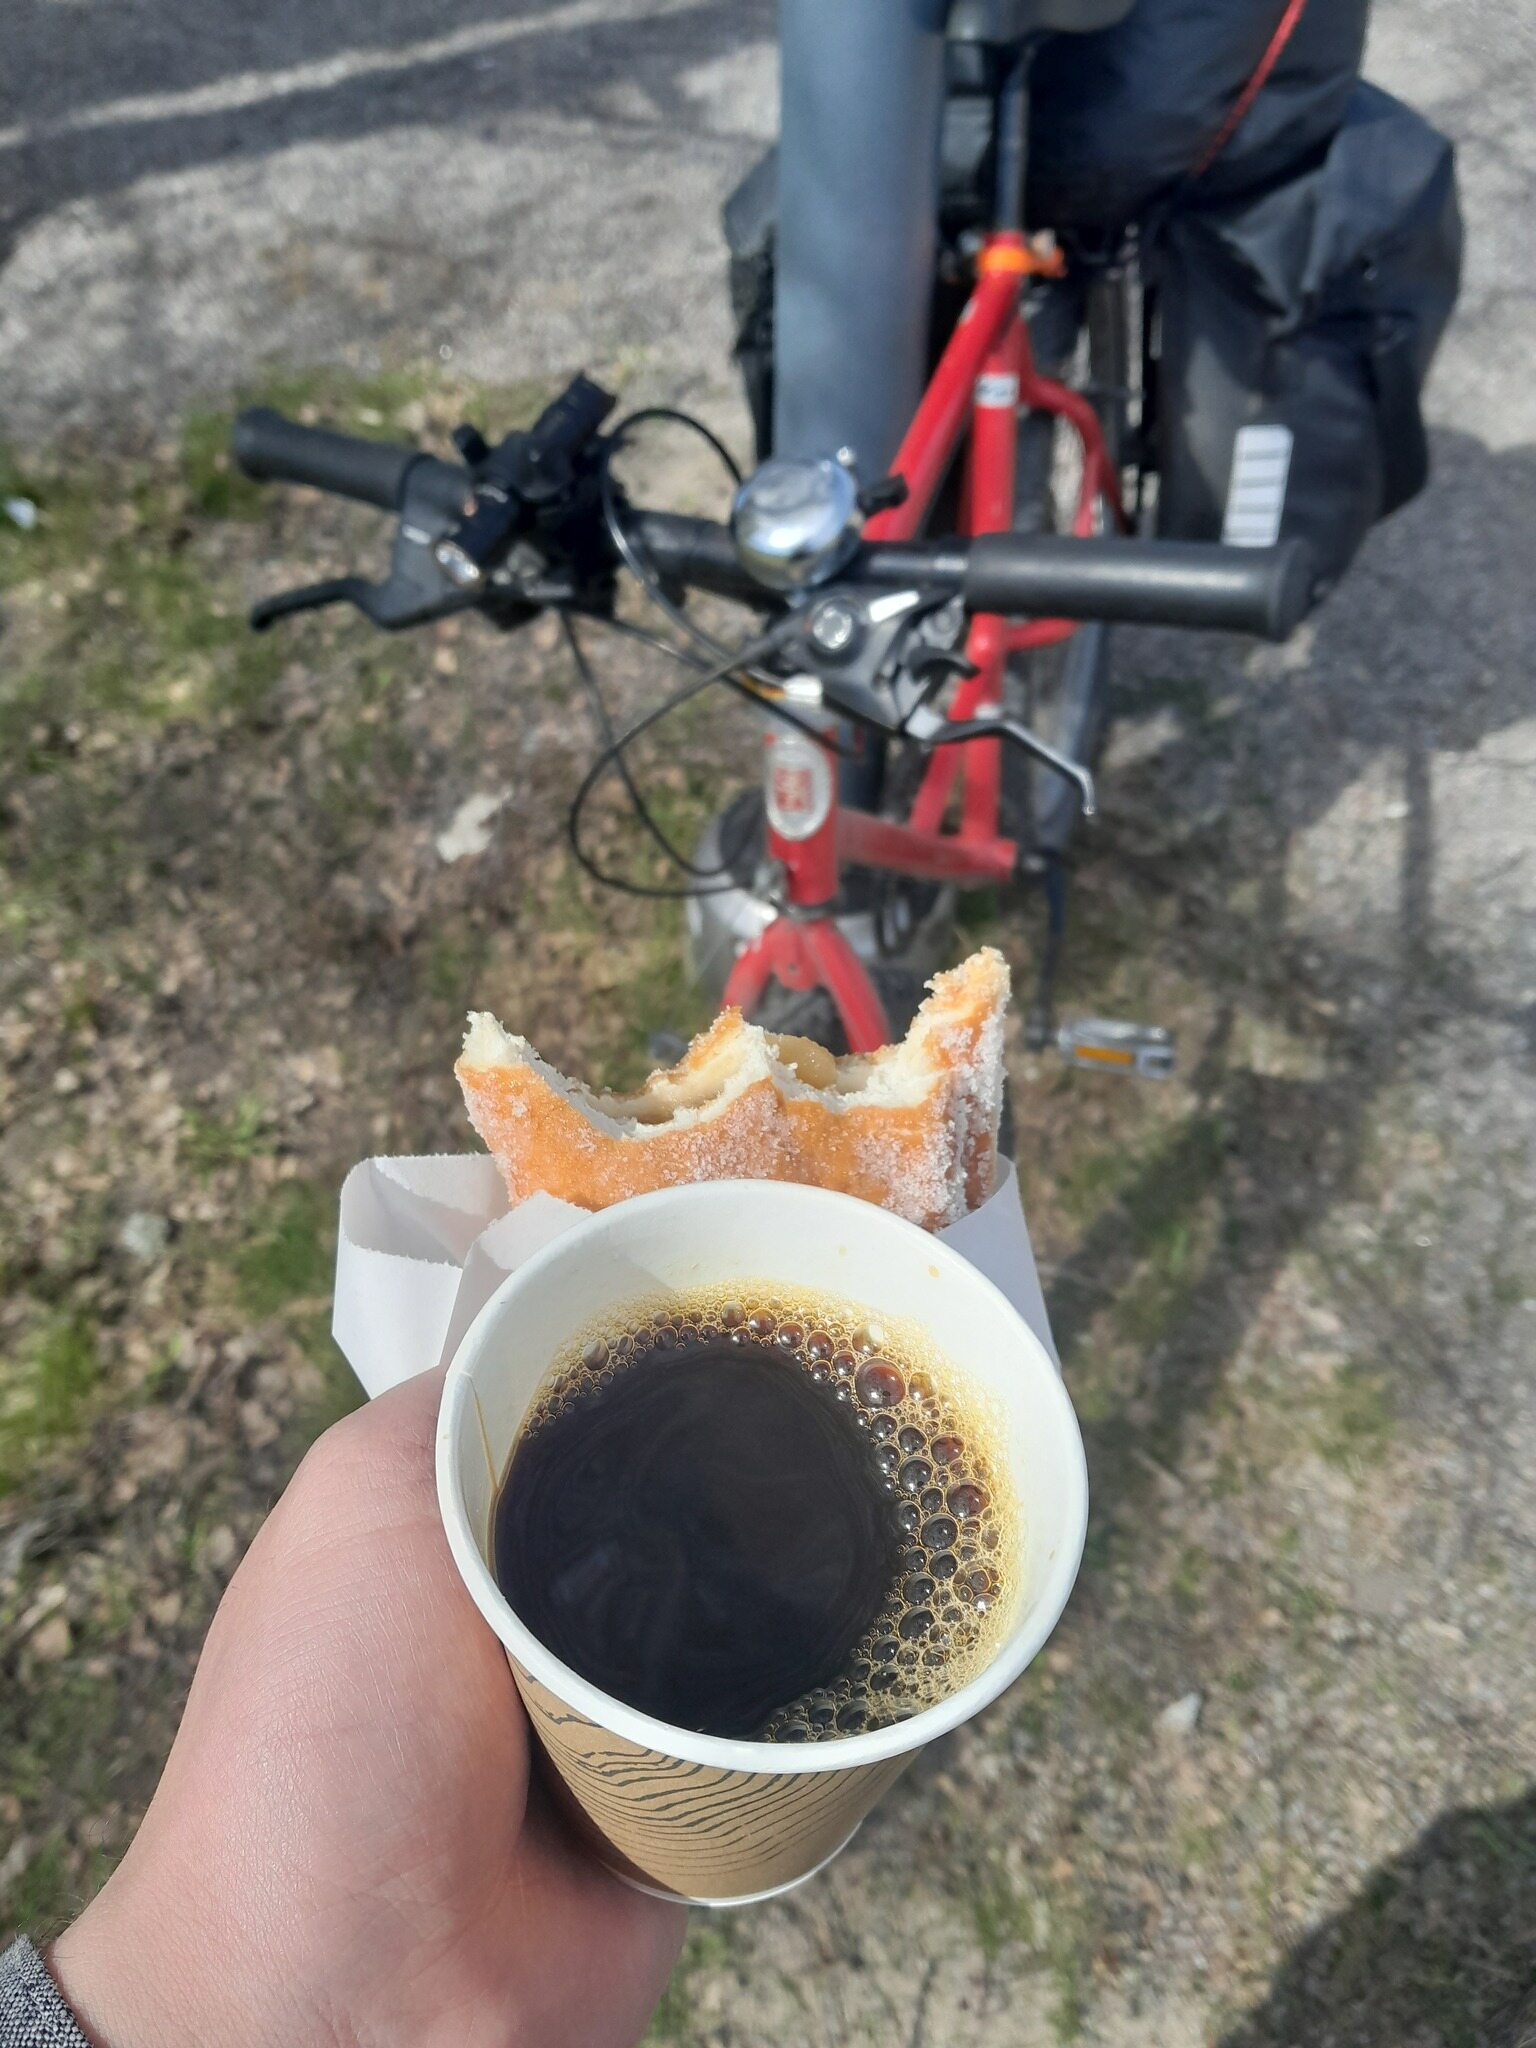
\includegraphics[width=1.05\linewidth]{assets/pyörävaellus25}
		\noindent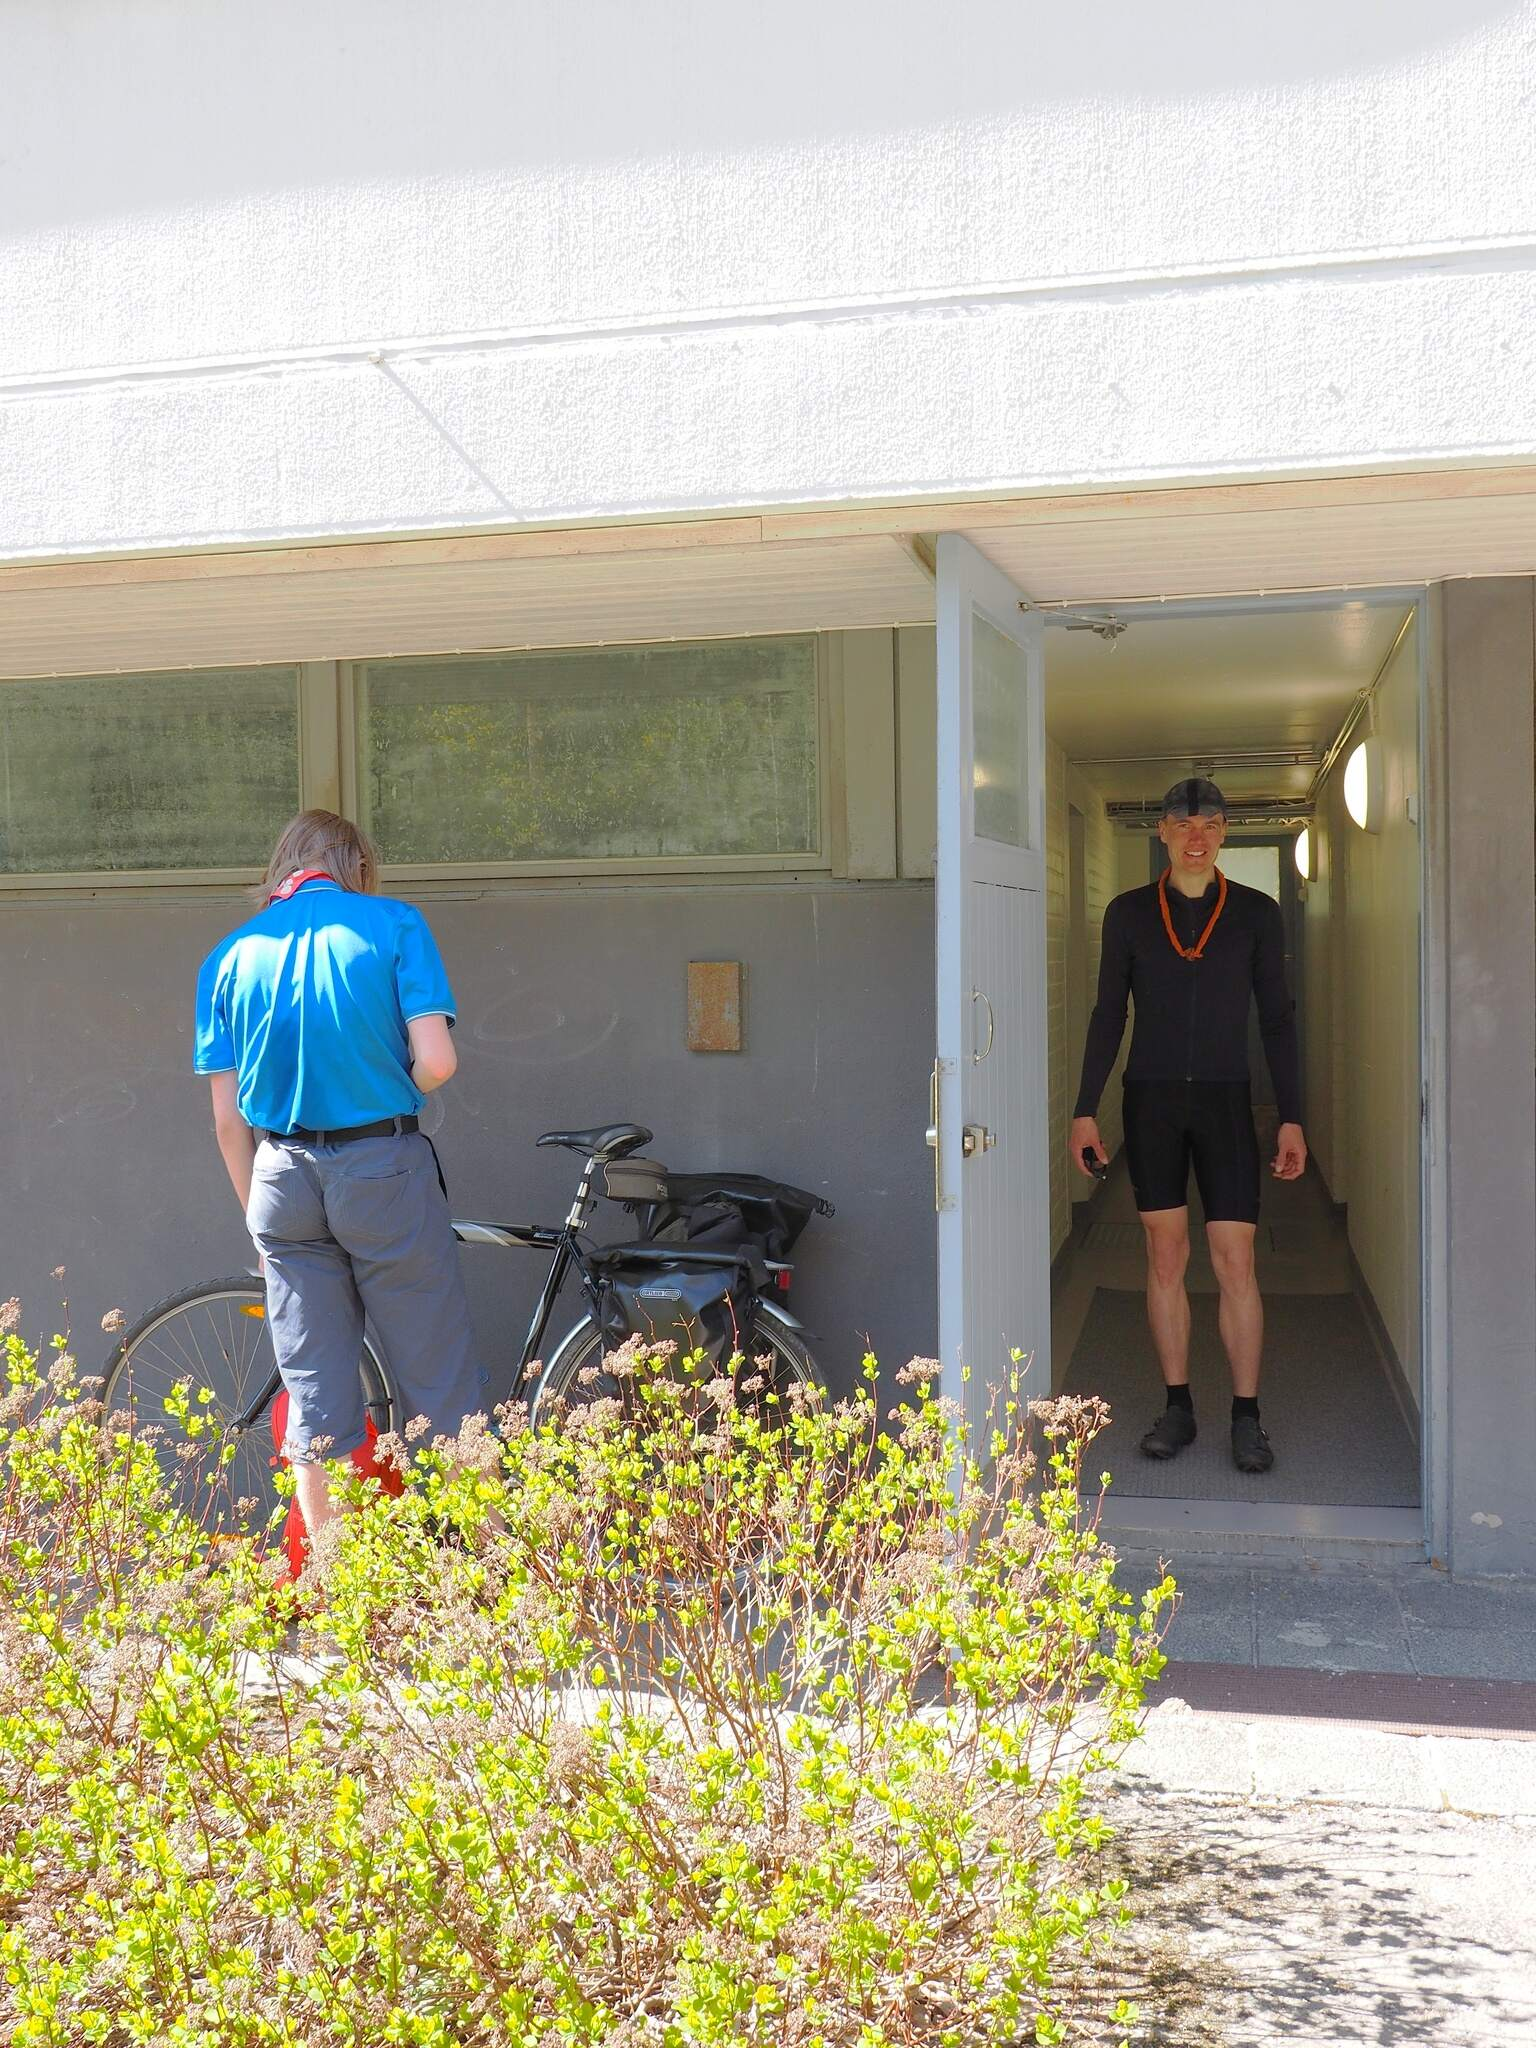
\includegraphics[width=1.05\linewidth]{assets/pyörävaellus26}
	\end{center}
	\columnbreak
	\vspace*{0.32cm}
	\begin{center}
		\noindent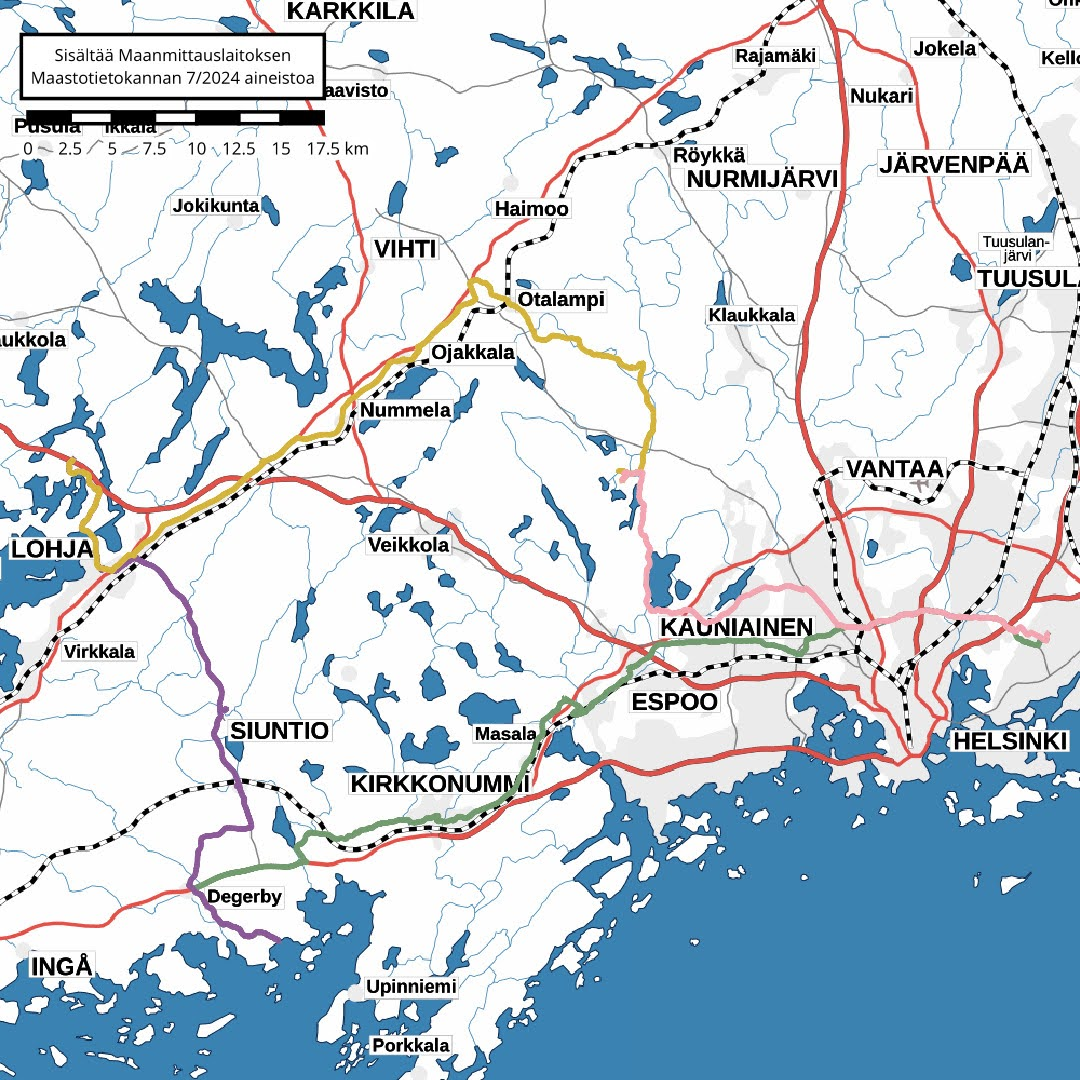
\includegraphics[width=1.05\linewidth]{assets/pyörävaellus27}
	\end{center}
	\vspace*{2cm}
	\begin{addmargin}[0.32cm]{0cm}
		{\small
		Neljäs ja viimeinen päivä meni nopeasti ja meillä oli ''vain'' 39~km
		jäljellä Kontulaan.
		Skipattiin lounas ja otettiin sen sijaan muutaman
		välipalatauko. Nopeammin kuin osaisimme uskoa olimme jo takaisin
		varastolla, yhteensä 224~km takanamme!
		}
	\end{addmargin}
\end{multicols}
\vspace*{-0.32cm}


\medskip
\noindent\null\hfill Tanguy Gérôme
